%%%%%%%%%%%%%%%%%%%%%%%%%%%%%%%%%%%%%%%%%
% Masters/Doctoral Thesis 
% LaTeX Template
% Version 2.5 (27/8/17)
%
% This template was downloaded from:
% http://www.LaTeXTemplates.com
%
% Version 2.x major modifications by:
% Vel (vel@latextemplates.com)
%
% This template is based on a template by:
% Steve Gunn (http://users.ecs.soton.ac.uk/srg/softwaretools/document/templates/)
% Sunil Patel (http://www.sunilpatel.co.uk/thesis-template/)
%
% Template license:
% CC BY-NC-SA 3.0 (http://creativecommons.org/licenses/by-nc-sa/3.0/)
%
%%%%%%%%%%%%%%%%%%%%%%%%%%%%%%%%%%%%%%%%%

%----------------------------------------------------------------------------------------
%	PACKAGES AND OTHER DOCUMENT CONFIGURATIONS
%----------------------------------------------------------------------------------------

\documentclass[
11pt, % The default document font size, options: 10pt, 11pt, 12pt
%oneside, % Two side (alternating margins) for binding by default, uncomment to switch to one side
english, % ngerman for German
singlespacing, % Single line spacing, alternatives: onehalfspacing or doublespacing
%draft, % Uncomment to enable draft mode (no pictures, no links, overfull hboxes indicated)
%nolistspacing, % If the document is onehalfspacing or doublespacing, uncomment this to set spacing in lists to single
%liststotoc, % Uncomment to add the list of figures/tables/etc to the table of contents
%toctotoc, % Uncomment to add the main table of contents to the table of contents
%parskip, % Uncomment to add space between paragraphs
%nohyperref, % Uncomment to not load the hyperref package
headsepline, % Uncomment to get a line under the header
%chapterinoneline, % Uncomment to place the chapter title next to the number on one line
%consistentlayout, % Uncomment to change the layout of the declaration, abstract and acknowledgements pages to match the default layout
]{MastersDoctoralThesis} % The class file specifying the document structure

%\usepackage[hyphens]{url}
\usepackage{setspace}
\usepackage{float}
\usepackage{subcaption}
%\usepackage{showframe}
\usepackage{microtype}
\usepackage{threeparttable}
\usepackage{graphicx}
\usepackage{adjustbox}
\usepackage[utf8]{inputenc} % Required for inputting international characters
\usepackage[T1]{fontenc} % Output font encoding for international characters
\usepackage{verbatim} % for comments
\usepackage{palatino} % Use the Palatino font by default
\usepackage{enumitem}
\usepackage[backend=bibtex,style=numeric,natbib=true,doi=false,isbn=false,url=false,maxbibnames=9,maxcitenames=1,sortcites=true,sorting=nyt]{biblatex} 
\usepackage{booktabs}
\usepackage[autostyle=true]{csquotes} % Required to generate language-dependent quotes in the bibliography
\usepackage[colorinlistoftodos,prependcaption,textsize=tiny]{todonotes}

\addbibresource{references.bib} % mendeley

% TODO disable hyphenation (for docx)
% \usepackage[none]{hyphenat}
% \usepackage[document]{ragged2e} 
% \raggedleft

%----------------------------------------------------------------------------------------
%	MARGIN SETTINGS
%----------------------------------------------------------------------------------------

\geometry{
	paper=a4paper, % Change to letterpaper for US letter
	inner=2.5cm, % Inner margin
	outer=3.8cm, % Outer margin
	bindingoffset=0.5cm, % Binding offset
	top=1.5cm, % Top margin
	bottom=1.5cm, % Bottom margin
	%showframe, % Uncomment to show how the type block is set on the page
}

%----------------------------------------------------------------------------------------
%	THESIS INFORMATION
%----------------------------------------------------------------------------------------

\thesistitle{The Social AR Continuum:\\
Wearable AR for Sharing Social Experiences} % Your thesis title, this is used in the title and abstract, print it elsewhere with \ttitle
\supervisor{
Prof. Robert W. \textsc{Lindeman}\\
Prof. Mark \textsc{Billinghurst}\\
Dr. Gun \textsc{Lee}\\
Assoc. Prof. Tobias \textsc{Langlotz}
} % Your supervisor's name, this is used in the title page, print it elsewhere with \supname

\examiner{} % Your examiner's name, this is not currently used anywhere in the template, print it elsewhere with \examname
\degree{Doctor of Philosophy} % Your degree name, this is used in the title page and abstract, print it elsewhere with \degreename
\author{Alaeddin \textsc{Nassani}} % Your name, this is used in the title page and abstract, print it elsewhere with \authorname
\addresses{} % Your address, this is not currently used anywhere in the template, print it elsewhere with \addressname

\subject{} % Your subject area, this is not currently used anywhere in the template, print it elsewhere with \subjectname
\keywords{} % Keywords for your thesis, this is not currently used anywhere in the template, print it elsewhere with \keywordnames
\university{\href{http://www.canterbury.ac.nz}{University of Canterbury}} % Your university's name and URL, this is used in the title page and abstract, print it elsewhere with \univname
\department{\href{http://hitlabnz.org/}{HIT Lab NZ}} % Your department's name and URL, this is used in the title page and abstract, print it elsewhere with \deptname
% \group{} % Your research group's name and URL, this is used in the title page, print it elsewhere with \groupname
\faculty{\href{http://www.canterbury.ac.nz/engineering/}{College of Engineering}} % Your faculty's name and URL, this is used in the title page and abstract, print it elsewhere with \facname

\AtBeginDocument{
\hypersetup{pdftitle=\ttitle} % Set the PDF's title to your title
\hypersetup{pdfauthor=\authorname} % Set the PDF's author to your name
\hypersetup{pdfkeywords=\keywordnames} % Set the PDF's keywords to your keywords
}

\begin{document}

\frontmatter % Use roman page numbering style (i, ii, iii, iv...) for the pre-content pages

\pagestyle{plain} % Default to the plain heading style until the thesis style is called for the body content

%----------------------------------------------------------------------------------------
%	TITLE PAGE
%----------------------------------------------------------------------------------------

\begin{titlepage}
\begin{center}

\vspace*{.06\textheight}
{\scshape\LARGE \univname\par}\vspace{1.5cm} % University name
\textsc{\Large Doctoral Thesis}\\[0.5cm] % Thesis type

\HRule \\[0.4cm] % Horizontal line
{\huge \bfseries \ttitle\par}\vspace{0.4cm} % Thesis title
\HRule \\[1.5cm] % Horizontal line
 
\begin{minipage}[t]{0.4\textwidth}
\begin{flushleft} \large
\emph{Author:}\\
{\authorname} % Author name - remove the \href bracket to remove the link
\end{flushleft}
\end{minipage}

\begin{minipage}[t]{0.4\textwidth}
    \begin{flushright} \large
    \emph{Supervisors:} \\
    {\supname} % Supervisor name - remove the \href bracket to remove the link  
    \end{flushright}
\end{minipage}\\[3cm]
 
\vfill

\large \textit{A thesis submitted in fulfilment of the requirements\\ for the degree of \degreename}\\[0.3cm] % University requirement text
\textit{in the}\\[0.4cm]
\deptname\\[2cm] % Research group name and department name
 
\vfill

{\large \today}\\[4cm] % Date
%\includegraphics{Logo} % University/department logo - uncomment to place it
 
\vfill
\end{center}
\end{titlepage}

% TODO: remove this 
\listoftodos

%----------------------------------------------------------------------------------------
%	DECLARATION PAGE
%----------------------------------------------------------------------------------------

\begin{declaration}
\addchaptertocentry{\authorshipname} % Add the declaration to the table of contents
\noindent I, \authorname, declare that this thesis titled, \enquote{\ttitle} and the work presented in it are my own. I confirm that:

\begin{itemize} 
\item This work was done wholly or mainly while in candidature for a research degree at this University.
\item Where any part of this thesis has previously been submitted for a degree or any other qualification at this University or any other institution, this has been clearly stated.
\item Where I have consulted the published work of others, this is always clearly attributed.
\item Where I have quoted from the work of others, the source is always given. With the exception of such quotations, this thesis is entirely my own work.
\item I have acknowledged all main sources of help.
\item Where the thesis is based on work done by myself jointly with others, I have made clear exactly what was done by others and what I have contributed myself.
\end{itemize}
 
\noindent Signed:\\
\rule[0.5em]{25em}{0.5pt} % This prints a line for the signature
 
\noindent Date:\\
\rule[0.5em]{25em}{0.5pt} % This prints a line to write the date
\end{declaration}

\cleardoublepage

%----------------------------------------------------------------------------------------
%	QUOTATION PAGE
%----------------------------------------------------------------------------------------

\vspace*{0.2\textheight}

\noindent\enquote{\itshape Thanks to my solid academic training, today I can write hundreds of words on virtually any topic without possessing a shred of information, which is how I got a good job in journalism.}\bigbreak

%----------------------------------------------------------------------------------------
%	ABSTRACT PAGE
%----------------------------------------------------------------------------------------

\begin{abstract}
\addchaptertocentry{\abstractname} % Add the abstract to the table of contents

% Abstract: In general, your abstract should give a more complete summary of the thesis (not the work). This means that you should have at least one sentence for each chapter, and there should be more details about the summary of your results. You get close in the last few sentences here, but more detail will be needed. I'm actually confuse that you are writing the Abstract FIRST! Usually it is the LAST thing you write.

The primary goal of this thesis is to develop and evaluate novel interaction techniques for enhancing Augmented Reality (AR) wearable headsets focusing on how we can use them to share social experiences with our family and friends. The motivation for this research comes from the need for more intuitive and natural approaches to sharing our social experiences in life using wearable AR headset that increase our social and co-presences. 
% Rob: Is this software, or the Social Continuum? What kind of Framework do you mean?
With a framework for sharing social experiences on wearable devices including panorama, live-video and 3D surrounding environment
% Rob: Are these three orthogonal? Why list them here? Is this all of them?
, we discuss advantages and limitations of various implementations and techniques of sharing social experiences using these media.  

Based on Human-Computer Interaction methodologies, we designed and conducted user studies to test and evaluate user presence and system usability of our implementation in sharing and annotating social experiences on AR headsets. We developed the concept of the Social AR Continuum which describes the space of sharing experiences on AR in various dimensions. We focused on the essential dimensions of "representing contacts", "sharing data" and "annotation", and developed user interfaces on these dimensions and evaluated them using user studies. 

The user study evaluation results show that using AR to share social experiences can increase users' presence. We also studied various ways to represent social contacts on AR in a focus group and user study, and show the user preference of the interface. We also summarise the results as design recommendations to help interface designers for designing shared experience on wearable AR systems. 

% Content: Can you insert in this where each of the user studies will be discussed? Also, don't you think the Social AR Continuum deserves its own chapter? Seems like one of the main topics of the thesis, and something you can attach your name to, so it should be highlighted. Also, there you can outline many possible axes, then go deep on the three you have chosen to explore. This indicates fertile areas that others can explore within the Continuum.

\end{abstract}


%----------------------------------------------------------------------------------------
%	ACKNOWLEDGEMENTS
%----------------------------------------------------------------------------------------

\begin{acknowledgements}
\addchaptertocentry{\acknowledgementname} % Add the acknowledgements to the table of contents
The acknowledgements and the people to thank go here, don't forget to include your project advisor\ldots
\end{acknowledgements}


%----------------------------------------------------------------------------------------
%	PREFACE
%----------------------------------------------------------------------------------------

\begin{preface}
\addchaptertocentry{\prefacename} % Add the preface to the table of contents

The research described in this dissertation has generated the following publications, which have appeared in the indicated peer-reviewed conference proceedings:

\preto\fullcite{\AtNextCite{\defcounter{maxnames}{99}}}

\noindent
\textbf{Chapter~\ref{ch:continuum} Social AR Continuum}
\begin{itemize}
    \item{ \fullcite{Nassani2017a}}
\end{itemize}

\noindent
\textbf{Chapter~\ref{ch:contacts} Social Contacts in AR}
\begin{itemize}
    \item{ \fullcite{Nassani2017b}}
    \item{ \fullcite{Nassani2017a}}
\end{itemize}

\noindent
\textbf{Chapter~\ref{ch:data} Social Data in AR}
\begin{itemize}
    \item{ \fullcite{Nassani2018a}}
    \item{ \fullcite{Nassani2018b}}
    % \item{ \fullcite{Nassani2018c}} --rejected
\end{itemize}

\noindent
\textbf{Chapter~\ref{ch:annotation} Social Interactions in AR}
\begin{itemize}
    \item{ \fullcite{Nassani2016}}
    \item{ \fullcite{Nassani2015}}
    % \item{ \fullcite{Nassani2015a}}    
    \item{ \fullcite{Reichherzer2014}}
    % \item{ \fullcite{Billinghurst2014}}
\end{itemize}

\end{preface}


%----------------------------------------------------------------------------------------
%	LIST OF CONTENTS/FIGURES/TABLES PAGES
%----------------------------------------------------------------------------------------
% \setcounter{tocdepth}{1}
\tableofcontents % Prints the main table of contents
\listoffigures % Prints the list of figures
\listoftables % Prints the list of tables

%----------------------------------------------------------------------------------------
%	ABBREVIATIONS
%----------------------------------------------------------------------------------------

\begin{abbreviations}{ll} % Include a list of abbreviations (a table of two columns)

% \textbf{LAH} & \textbf{L}ist \textbf{A}bbreviations \textbf{H}ere\\
% \textbf{WSF} & \textbf{W}hat (it) \textbf{S}tands \textbf{F}or\\

\textbf{AR} & \textbf{A}ugmented \textbf{R}eality\\
\textbf{CCS} & \textbf{C}amera \textbf{C}oordinate \textbf{S}ystem\\
\textbf{DOF} & \textbf{D}egrees \textbf{O}f \textbf{F}reedom\\
\textbf{FPS} & \textbf{F}rames \textbf{P}er \textbf{S}econd\\
\textbf{HMD} & \textbf{H}ead \textbf{M}ounted \textbf{D}isplay\\
\textbf{HCI} & \textbf{H}uman-\textbf{C}omputer \textbf{I}nteraction\\
\textbf{UI} & \textbf{U}ser \textbf{I}nterface\\

\end{abbreviations}

%----------------------------------------------------------------------------------------
%	PHYSICAL CONSTANTS/OTHER DEFINITIONS
%----------------------------------------------------------------------------------------

% \begin{constants}{lr@{${}={}$}l} % The list of physical constants is a three column table

% % The \SI{}{} command is provided by the siunitx package, see its documentation for instructions on how to use it

% Speed of Light & $c_{0}$ & \SI{2.99792458e8}{\meter\per\second} (exact)\\
% %Constant Name & $Symbol$ & $Constant Value$ with units\\

% \end{constants}

%----------------------------------------------------------------------------------------
%	SYMBOLS
%----------------------------------------------------------------------------------------

% \begin{symbols}{lll} % Include a list of Symbols (a three column table)

% $a$ & distance & \si{\meter} \\
% $P$ & power & \si{\watt} (\si{\joule\per\second}) \\
% %Symbol & Name & Unit \\

% \addlinespace % Gap to separate the Roman symbols from the Greek

% $\omega$ & angular frequency & \si{\radian} \\

% \end{symbols}

%----------------------------------------------------------------------------------------
%	DEDICATION
%----------------------------------------------------------------------------------------

\dedicatory{To B\ldots} 

%----------------------------------------------------------------------------------------
%	THESIS CONTENT - CHAPTERS
%----------------------------------------------------------------------------------------

\mainmatter % Begin numeric (1,2,3...) page numbering

\pagestyle{thesis} % Return the page headers back to the "thesis" style
\setstretch{1.5} 

% Include the chapters of the thesis as separate files from the Chapters folder
% Uncomment the lines as you write the chapters

\chapter{Introduction}
\label{ch:intro}

This thesis explores how wearable Augmented Reality (AR) can be used to create new types of social experiences. AR is a technology that enables the seamless merging of the real world with virtual content (including visual and audio) so that both real and virtual can be seen and interacted with at the same time. Azuma defined AR as the coexistence of the virtual world and the real world, and that "\textit{it would appear to the user that the virtual and real objects coexisted in the same space}"~\cite{azuma1997survey}. Milgram defined the Mixed Reality (MR) continuum (Figure \ref{fig:mr-continuum}) and placed AR between 1) Virtual Reality (VR) where the user is fully immersed in virtual contents and 2) real environment without any augmentations \cite{Milgram1995a}. 

\begin{figure}[H]
    \centering
    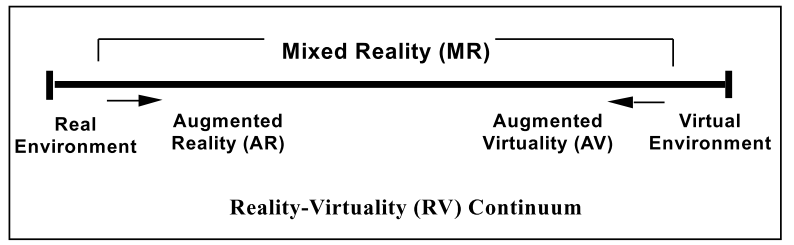
\includegraphics[width=0.8\linewidth]{images/10-intro/mixed-reality-continuum.png}
    \caption{The mixed reality continuum by Milgram \cite{Milgram1995a}}
    \label{fig:mr-continuum}
\end{figure}

We, as humans, are social creatures, and it is our way to stay connected with each other, communicating our identity and the feeling of relatedness to one another \cite{HuangWeidong2013}. Social interactions help to establish mutual understandings in collaborative scenarios and therefore, can be used as an effective measure of collaborative technology \cite{Li2013}. Social interactions have been influenced by technology. For instance, emoticons have been used in written communication instead of text to represent our emotions, intentions and cultural differences \cite{Pavalanathan2016}, and was found to be related to expressing emotions in face-to-face situations \cite{Derks2007}. 

One of the advantages of AR in communicating social dynamics is that it enables the user to interact with virtual content while keeping social connections with people around in the real world \cite{HuangWeidong2013}. Mobile AR facilitates shared spaces and experiences with remote users in a way that adds to social connections and increases user engagement. 

Having people contributing to AR content could improve the sense of community and inter-connectedness. However, when more information is shared, there is more risk of reducing the sense of privacy \cite{Olsson2013}. In a study of social interaction and mobility in AR games, \textcite{Schmalstieg_144} found that players of mobile AR games are more likely to interact with each other socially and physically, which improves the enjoyment of AR experience. AR could improve social interactions by making people more connected with each other and excited about sharing virtual experiences and making the social experience more rich with additional virtual content. 

In a review of the trends of 20 years research in AR at ISMAR\footnote{http://www.ismar.net/}, \textcite{Zhou2008, Kim2018} reported that "\textit{AR technology will continue to develop even more dynamically and effectively over the next ten years, toward the vision of pervasive presence in our daily lives.}" \cite{Kim2018}. AR displays are getting more affordable with better rendering and registration techniques. They are also becoming more self-contained and lighter, which enables mobile AR applications.

According to a review about the historical uses of wearable displays and AR displays \cite{Peddie2017}, it started in 1940 with the first heads-up display (HUD) in the UK. Then in the 1960s, most uses of AR were to build an AR helmet for the pilot's field of view. Then the interest in AR started increasing In 2007/8 the first GPS enabled phones became available, enabling outdoor AR, and then the iphone and android devices became powerful enough for computer vision tracking on the handset. Then interest in AR started increasing in 2009 when Lego\footnote{https://www.lego.com} introduced AR Digital box, then started a relative decline around when Google Glass was introduced in 2012. The Gartner 2019 trends report \cite{gartner2019} showed that AR and immersive technologies have been getting out the "disillusionment" phase of the hype cycle and are moving toward steady adoption and day to day scenarios in the next 5-10 years.

\section{Problem Statement}

With the rapid development of technology and the potential use of AR in everyday life, this thesis aims to study the future challenges in social AR. The focus of this thesis is on enabling the use of wearable AR for sharing social experiences. The gap between the vision of social AR and the current state of the art is that state of the art in AR research has focused on task-oriented collaborative AR more than social AR. Initial attempts at exploring social AR in 2013 (at the beginning of this thesis) were limited in terms of the number of users. 
% This thesis explores how multiple people would use social AR to connect the shared virtual space and the interaction techniques. 

This PhD thesis addresses the problems of: 
\begin{enumerate}
    \item visualising and interacting with social contacts through wearable AR displays.
    \item displaying a large amount of 3D content of sharing social data that is overlaid over a limited available physical space through wearable AR devices.
    \item defining and exploring the best ways to use wearable AR devices to connect with social networks.
\end{enumerate}

Previously, hand-held AR systems have been used to view social networks in different ways. For example, Presslite's Twitter 360\footnote{https://www.youtube.com/watch?v=5w7EAz8-uwU} (Figure \ref{fig:presslite}) shows virtual tweets overlaid on the real world at the locations of the people that sent them , and early versions of Junaio\footnote{https://en.wikipedia.org/wiki/Junaio} allowed people to drop virtual messages and pictures in the real world, as did the popular application Sekai Camera\footnote{https://www.youtube.com/watch?v=oxnKOQkWwF8}. Most of these applications were focused on asynchronous collaboration, enabling people to post virtual messages in space, which can later be browsed and retrieved by other users. 

\begin{figure}
    \centering
    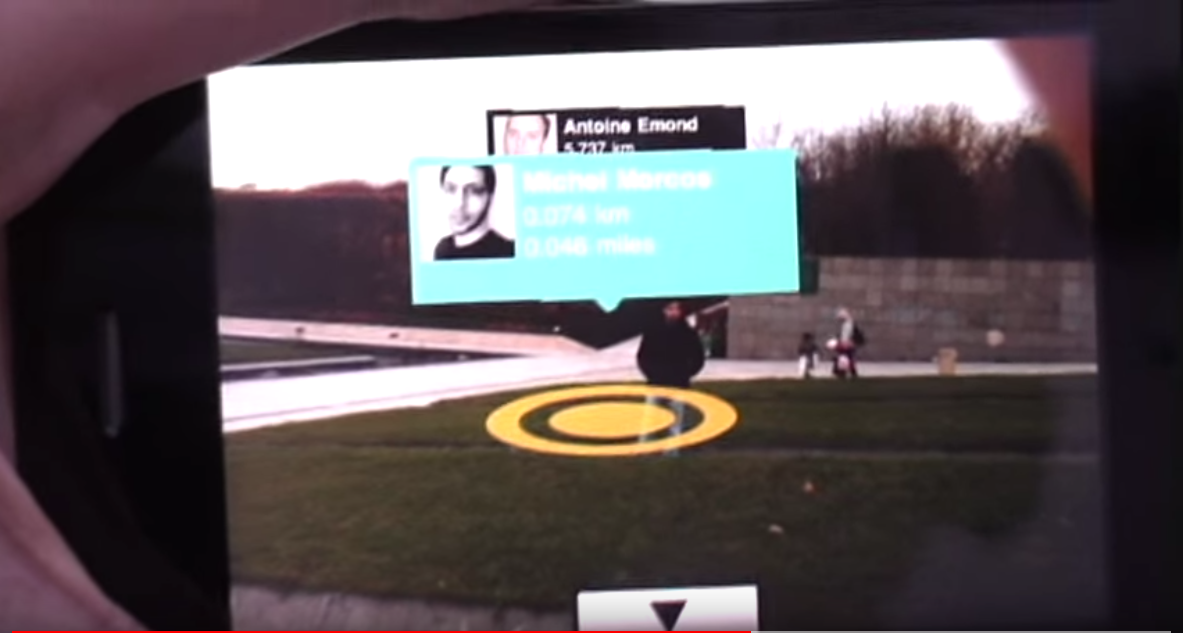
\includegraphics[width=0.8\linewidth]{images/10-intro/Presslite-twitter-360.PNG}
    \caption{Presslite's Twitter 360 AR interface by Twitter in 2009}
    \label{fig:presslite}
\end{figure}

However, similar technology could also be used for live synchronous collaboration such as live video avatar sharing~\cite{Billinghurst2002}, sharing realistic 3D models superimposed over the real world~\cite{Fanello2016}, or by using virtual avatars to show a live view of remote collaborators and their surrounding space as in the Holoportation system~\cite{Fanello2016} (Figure \ref{fig:holoportation}).

\begin{figure}
    \centering
    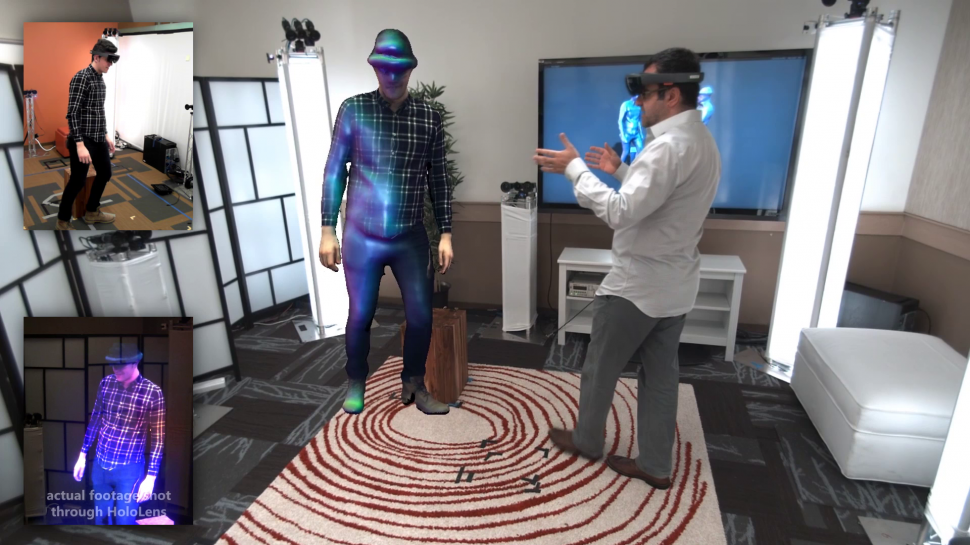
\includegraphics[width=0.8\linewidth]{images/10-intro/holoportation.png}
    \caption{Holoportation by Microsoft \cite{Fanello2016}}
    \label{fig:holoportation}
\end{figure}

% - The potential for AR to be a social sharing platform. \\
% - Sharing social experiences was not fully addressed in the research community

With major industry players (e.g., Microsoft, Facebook and Magic Leap) building solutions in AR, there is potential for use of AR in social networks. Just as people today use their mobile phones to connect with hundreds or thousands of friends, wearable AR displays could be used to connect with friends and view and interact with their shared information.

Applications for Social VR and 360-degree video have been introduced on new VR headsets. For instance, Facebook Spaces\footnote{https://www.facebook.com/spaces} allows VR users to connect with friends and family and share 360-degree photos and take selfies. Altspace VR\footnote{https://altvr.com/} is a social VR application which was acquired by Microsoft and has been extended to support different hand-held and wearable devices to be used for social connection with others. Most recently, Magic Leap's Avatar Chat\footnote{https://www.magicleap.com/stories/blog/connect-with-friends-with-avatar-chat}(Figure \ref{fig:ml-avatar-chat-1}) offers similar experiences where avatars representing social friends are displayed in an AR space. 

\begin{figure}
    \centering
    
\includegraphics[width=0.8\linewidth]{images/10-intro/magic-leap-avatar-chat.jpg}
    \caption{Avatar Chat by Magic Leap, 2018}
    \label{fig:ml-avatar-chat-1}
\end{figure}

By using a wearable AR display like the Microsoft HoloLens\footnote{https://www.microsoft.com/en-nz/hololens}, it could be possible for the user to see an AR representation of their social network visible at all times. However, this raises the question of how to visually represent the user's contacts in the network. For example, if a user has lots of friends in their social network, visually representing each of them might clutter the user's visual space.

The limitation of prior work is that until recently (2018), there was no comprehensive analysis of the social AR space and no sufficient exploration of sharing social experiences on wearable AR. It is easy to imagine that in the future it will be possible for wearable AR systems to be used to capture and share a 3D view of the user's surroundings with hundreds or thousands of followers on a social network. However, before this becomes commonplace, many important research questions need to be addressed. For example, would a person be comfortable sharing a view of their surrounding real space with relative strangers? This work aims to explore how wearable AR systems could share a user's surrounding room environment with social contacts and to measure how comfortable the sharer and the viewer would feel regarding privacy within different interface options. 

If AR is to be used to represent contacts in social networks, there could be a large number of contacts to show. This research has benefited from earlier work on different ways of managing large amounts of information in AR interfaces. In the following section, this thesis outlines the research questions based on the above problem space and the gap identified in previous work.

\section{Research Questions}

This thesis targets the future where headworm AR devices are used every day, and social networks are visualised in the AR view. The overarching research question is \textit{how can AR be used for sharing social experiences in both remote and face to face social contacts}. This thesis addresses the following research questions: 

\begin{enumerate}[label=RQ\arabic*]
    % (chapter 3 - Social AR Continuum)
    \item{\label{rq:continuum}
    What are the dimensions/factors/parameters in sharing social experiences on wearable AR devices?
    % \\(option 1): How to represent social networks and shared social data on wearable AR devices?
    % \\(option 2): What dimensions/factors/parameters in sharing social experiences on wearable AR devices?
    }
    % (chapter 4 - visualising social contacts) 
    \item{\label{rq:people}
    What dimensions work best for visualising and interacting with social contacts through wearable AR displays?
    % \\(option 1): How to visualise our social contacts as virtual avatars on wearable AR devices?
    % \\(option 2): What are the options of visualising contacts on social AR?
    % \\(option 3): How visualising social contacts are placed on the Social AR Continuum?
    % \\(option 4): What is the impact of visualising social contacts on social presence?
    % \\(option 5): What is the impact on social presence of different visualisation methods for social contacts?
    }
    % (chapter 5 - Social data continuum)
    \item{\label{rq:data}
    How does social proximity affect visualising and interaction with shared social data on wearable AR displays?
    % What dimensions are best to visualise and interact with shared social data on wearable AR displays?
    % What is the best way to view and interact with shared social data on AR displays?
    % \\(option 1): How to share virtual objects/data with our social network on wearable AR devices?
    % \\(option 2): What are the options of sharing social data in AR?
    % \\(option 3): How sharing data is placed on the Social AR Continuum?
    }
    % (chapter 4 - social interaction continuum)
    \item{\label{rq:interaction}
    How can wearable AR displays be used best for interacting with social contacts and shared social data?
    % \\(option 1): How to represent annotations/tags on wearable AR devices for shared social experiences?
    % \\(option 2): How annotations/tags are used as an interaction method in social AR? 
    % \\(option 3): What are the options/parameters of annotation that can be changed in social AR?
    }
\end{enumerate}

In order to answer the research questions, this thesis explores how wearable AR can be used for sharing social experiences. These explorations identified the parameters through which AR sharing for social reasons happens. Once the parameters were defined, system prototypes were built as a proof of concept of how users can experience those dimensions. User studies were approved by the Human Ethics Committee (HEC) and aimed to test the objectives of each system with human participants. Outcomes of user studies include subjective and objective measures and observations of users' behaviour and feedback from going through these experiments. 

Chapter \ref{ch:continuum}: "The Social AR Continuum" aims to answer \ref{rq:continuum} with describing the overall dimensions of the Social AR Continuum. 
Chapter \ref{ch:contacts} "Visualising Social Contacts" aims to answer \ref{rq:people} by exploring visualising social contacts. 
Chapter \ref{ch:data} "Sharing Data Continuum" focuses more on the data being shared with social contacts and aiming to answer \ref{rq:data}.
Chapter \ref{ch:annotation} "Annotation Continuum" aims to answer \ref{rq:interaction} with exploring annotations and tags for sharing social experience. 

\section{Contributions}

The following summarises the main contributions of this thesis: 

\begin{itemize}
    \item The parameters and dimensions of the Social AR Continuum were identified. The main contribution is defining the Social AR Continuum, which consists of a set of parameters that define the space of sharing social experiences through wearable/hand-held AR devices. Following the identification, this thesis defines the space of the Social AR Continuum by exploring the main parameters that can be varied based on social proximity. These parameters are grouped into the following categories 1) self and other, 2) shared objects \& surrounding environment and 3) interactions and annotations. Under each of these categories, this thesis defines the dimensions of variables that affect the shared social experience.
    
    \item Several social AR experiences in terms of user interfaces were implemented. For each dimension defined on the continuum, a system prototype was built to test the user interface design with human subjects. The implementation details are described in the thesis for future use.
    
    \item User studies were conducted to evaluate and validate the parameters of the Social AR Continuum. The prototypes then used in a series of user-studies and focus-groups were conducted to validate the dimensions of the Social AR Continuum.
    
    \item High-level design guidelines were synthesised for interface designers looking to build social sharing experiences on AR devices. One of the outcomes of defining the Social AR Continuum and validating these dimensions is that this work can serve as high-level experience design guidelines that help individuals and organisations to create effective AR experiences for social sharing and connection purposes.
\end{itemize}

In summary, this thesis helps to increase the understanding of how to share social experiences through AR devices. The results of the user experiments conducted throughout this research help identify the impact of the Social AR Continuum parameters on presence, user engagement and user interface usability, which serve as guidelines for future designs. 

Figure \ref{fig:thesis-outline} shows the structure of the thesis and how it answers the research questions. The thesis is organised as follows: Chapter \ref{ch:continuum} describes the Social AR Continuum and the parameters/dimensions involved. 
Chapter \ref{ch:contacts} focuses on the dimensions of self and others of representing social contact networks on AR devices. 
Chapter \ref{ch:data} studies the shared social data and surrounding environment dimensions, including shared 360-degree videos and 3D captured spaces. 
In chapter \ref{ch:annotation}, this thesis looks into the shared data and annotation continuum, including different implementations of shared annotation and awareness cues on different platforms (hand-held and wearable).


\begin{figure}
    \centering
    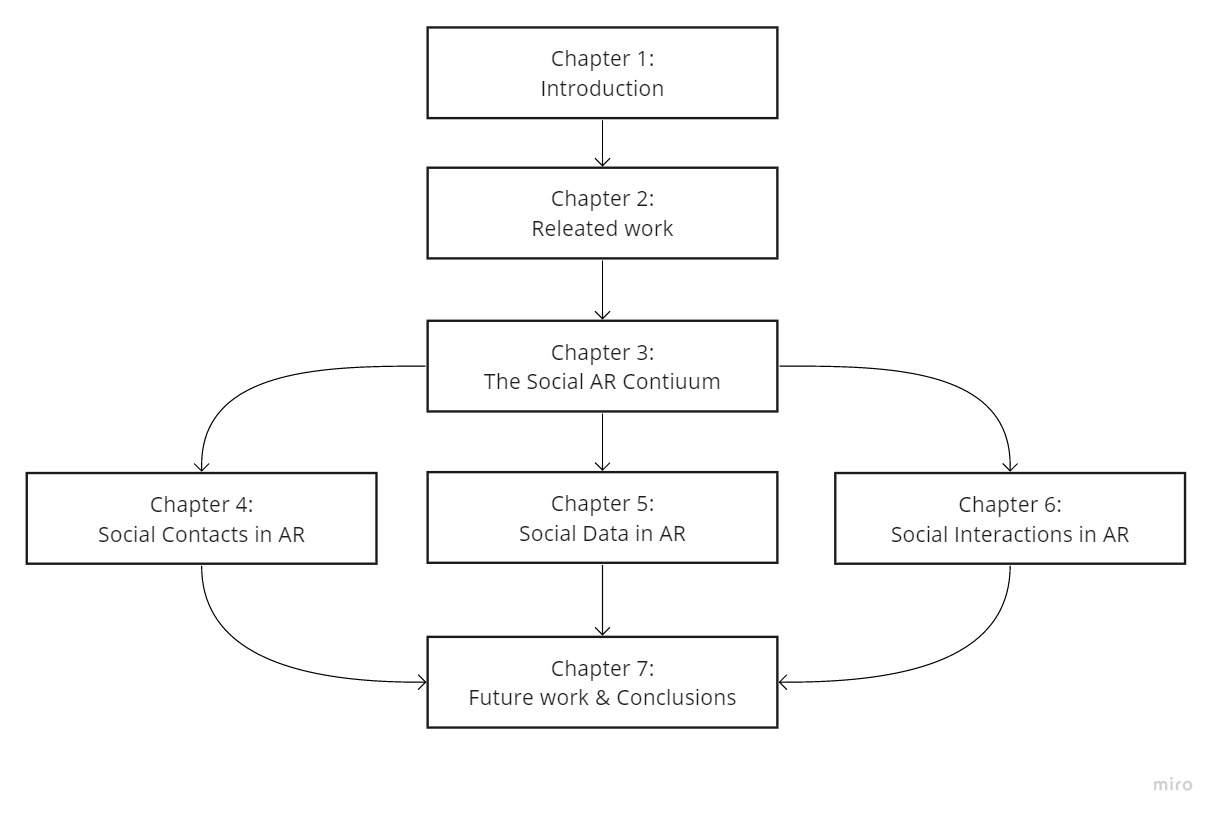
\includegraphics[width=\linewidth]{images/10-intro/thesis-outline.jpg}
    \caption{Thesis outline}
    \label{fig:thesis-outline}
\end{figure}

\section{Selected Publications}
\preto\fullcite{\AtNextCite{\defcounter{maxnames}{99}}}

Most of the work in this thesis has been submitted, peer-reviewed and published at scientific conferences and journals specialising in the AR, HCI and computer graphics fields. This list contains selected publications that are relevant to this thesis. 

The following publication defines the concept of the Social AR Continuum and describes a focus group and a user study implementing visualising social contacts through an AR headset, and addressing \ref{rq:continuum}. 

\begin{itemize}
    \item{ \fullcite{Nassani2017a}}
\end{itemize}

The following publications focus on visualising social contacts based on social proximity, addressing \ref{rq:people}. 

\begin{itemize}
    \item{ \fullcite{Nassani2017b}}
    \item{ \fullcite{Nassani2017}}
\end{itemize}

The following publications focus on shared surrounding environments and changing the levels of detail based on social proximity, addressing \ref{rq:data}.

\begin{itemize}
    \item{ \fullcite{Nassani2018a}}
    \item{ \fullcite{Nassani2018b}}
    % \item{ \fullcite{Nassani2018c}} -- frontier paper rejected
\end{itemize}


The following publications focus on placing AR annotations/tags on shared 360-degree panoramas and video streaming content, addressing \ref{rq:interaction}.

\begin{itemize}
    \item{ \fullcite{Nassani2016}}
    \item{ \fullcite{Nassani2015}}
    % \item{ \fullcite{Nassani2015a}}    
    \item{ \fullcite{Reichherzer2014}}
    % \item{ \fullcite{Billinghurst2014}}
\end{itemize}
The above publications help to answer the research questions of this thesis, including how to share social experiences on AR devices for each category on the Social AR Continuum. 

\chapter{Related Work}
\label{ch:background}

% \todo[inline]{Gun: Again, it feels like you need better grouping of the sections as in the current structure, many of them overlap with each other and it's a bit hard to see the logical flow of supporting why your thesis is important and how it fills in the research gap/limitation of the current state-of-the-art}

% \todo[inline]{Mark: This is important but probably should be in this section since it's not about virtual avatars. Maybe you need to have a section about information management, and discuss how these techniques could be used to manage avatar representations in Social AR.}

This work extends earlier work in wearable AR, AR annotation, social proximity, virtual avatars, research collaboration, telepresence, and sharing social experiences. This section examines previous related work on wearable AR, AR collaboration, and sharing social experiences from the social AR perspective. 

\section{Wearable AR} 

AR devices can be categorised into wearable (e.g., head-mounted displays, helmet or contact lenses), hand-held (e.g., phone, tablet) or projected displays where AR is projected onto a larger area regardless of where the user is looking~\cite{Peddie2017}. 

\textcite{Feiner1997a} presented the first mobile wearable AR system in 1997 called "Touring Machine" combining a head-mounted display (HMD), hand-held tablet, and a backpack carrying a computer GPS and radio for wireless access. This work was followed up by \textcite{Hollerer1999a} and explored different user interfaces on a wearable see-through display. The interface allowed users to sketch pathways and annotate their world for collaborative AR systems. 

Wearable AR has added an extra dimension to AR, allowing people to collaborate hands-free. \textcite{Feiner1999} talked about what impact wearable computing (and being mobile in general) has from the social perspective. These implications include personal privacy concerns, connectivity, collaboration, and how it looks and feels. 

Wearable AR has been explored for social interactions. For instance, \textcite{Cheok2002a} developed a city-wide wearable mixed reality social game, however the system was bulky to wear and they did not report on a user study. 

\textcite{Amores2015} used gestures to communicate social interactions via wearable devices. \textcite{Lee2019} used live 360 cameras to communicate between worker and helper. \textcite{Shu2018} developed a system of facial recognition to facilitate social interactions. 

With wearable AR devices becoming affordable, available and ubiquitous, there is a need to understand design considerations for this new platform. Previous research has looked into using AR headsets for collaborative use. For example in enhancing face-to-face \cite{Billinghurst2002} or remote collaboration \cite{Gupta2016}. The research presented here explores the use of AR headsets for social interaction and shared experiences. Social interactions can be extrapolated from current social network interactions where \enquote{friends} share content and interact with another's content (i.e., placing likes and comments).

\textcite{Dey2018} reviewed ten years of research in AR usability studies and highlighted the importance of user studies in AR research especially the social and environmental impact of user studies that take place in outdoor locations. Remote collaboration is one of the main categories of AR user studies, but surprisingly fewer than expected until 2014. They also reported on the increased availability of hand-held and wearable devices enabled for more research in this area. 

AR in remote collaboration was studied in to see if AR was enhancing task completion \cite{Kim2014, Tversky2015, Gupta2016, Kim2015}.
\textcite{hauber2008understanding} studied remote video collaboration focusing on the spatial interactions. In four experiments, the author measured the social presence, awareness, physical presence, co-presence, ease of use and efficiency between different conditions including immersive and virtual environments as well as standard video conferencing. Those experiments found higher social presence in video collaborative virtual environments compared to standard video conferencing. Also found that standard video or face to face collaboration was better than adding avatars in virtual collaboration.

% \todo[inline]{Again, what did you learn from these works? Your related-work section reads more like a laundry list of previous papers, rather than a set of papers that you read and learned something from, thereby informing your own choices and work. You've (rightfully) chosen to structure your related work section around larger themes, since this makes sense in terms of your own work. Now you need to help the reader understand what the papers you cite have done to help you.}

% There is a need to understand design considerations for this new platform. Previous research has looked into using wearable AR headsets for collaborative use, for example in enhancing face to face \cite{Billinghurst2002} or remote collaboration \cite{gupta2016you}. The research presented here explores the use of AR headsets for social interaction and shared experiences. 

\section{AR Annotation}

There are several examples of AR annotation demonstrations on mobile devices \cite{Wither2009a, Gauglitz2014, Larabi2018, Grasset2012}. For example, mobile AR browsers (e.g., Wikitude\footnote{https://www.wikitude.com/} or Junaio\footnote{https://en.wikipedia.org/wiki/Junaio}) can overlay AR tags in the real world using GPS and other motions sensors. While they were successful in demonstrating the concept of visualising AR annotation, the registration of virtual objects in the real world can be inaccurate, and they can only be used in outdoor, large-scale environments. Mobile AR browsers usually create AR tags in advance, but  AR research projects have investigated in situ and interactive creation of AR tags. For example, \textcite{Kim2011} presented an interactive method where the user stands in a fixed position to calibrate the room model with the gyroscope data. The user can then touch and annotate locations with a rectangle where virtual content, like text, images and 3D models, can be overlaid. 

A variety of AR annotation methods with wearable interfaces have also been presented. SixthSense \cite{Mistry2009a} used a wearable gestural interface for AR annotation. It consists of a camera and a small projector mounted on a hat or in a pendant. The camera tracks user hand gestures, and the projector visually augments virtual content onto the physical objects with which the user is interacting. However, the system requires planar surfaces in front of the user for accurate projection because of the lack of a depth sensor. OmniTouch \cite{Hollerer1999a} is a wearable projection system equipped with depth-sensing technology that enables interactive multi-touch applications on different surfaces. Both the depth camera and projector are mounted onto a form-fitting metal frame, which is worn on the shoulders, and secured with a chest strap. This system extends the typical scenarios supported by SixthSense to on-body surfaces or objects held in the hand for image projection. However, the system was still bulky and inconvenient to use because it needed to be connected to a desktop computer.

\section{Remote Collaboration}

\begin{figure}
    \centering
    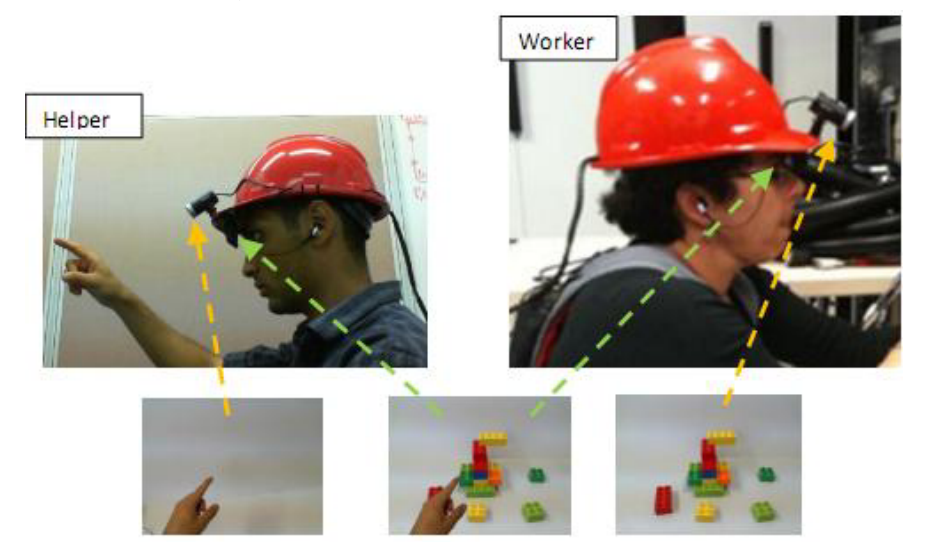
\includegraphics[width=\linewidth]{images/Huang2013.PNG}
    \caption{HandsInAir: A Wearable System for Remote Collaboration. The worker video stream their work environment to the helper. The helper stream their hand gestures to the worker during the remote collaboration session \cite{Huang2013}}
    \label{fig:HandsInAir}
\end{figure}

Camera-equipped mobile devices provide a quick way of capturing and sharing experiences and spaces. Wearable computers that combine HMDs and cameras provide new opportunities for collaboration. For example, the Google Glass\footnote{http://www.google.com/glass/} wearable system has a camera, microphone, and head-worn display.

There has been a significant amount of earlier research on remote collaboration using head-mounted cameras and displays. For example, allowing a remote user to place virtual annotations on the live camera view from a head-worn camera and showing the result in the wearers HMD, has been shown to enhance remote collaboration \cite{Fussell2003}. Other systems allow a remote user to place their hands in the local user's view \cite{Huang2013} (Figure \ref{fig:HandsInAir}). 

In many wearable and mobile AR applications, remote collaboration is the primary purpose of sharing a view of the user's world. For example, remote expert collaboration systems have been developed where a local worker with an AR display can share a live video view of their workspace with a remote expert (Figure \ref{fig:Billinghurst2002}) \cite{Billinghurst2002}. The remote expert can provide visual feedback with AR graphical cues.  However, most of these systems have just been developed for collaboration between small numbers of users, and not for more extensive social networks. 

\begin{figure}
    \centering
    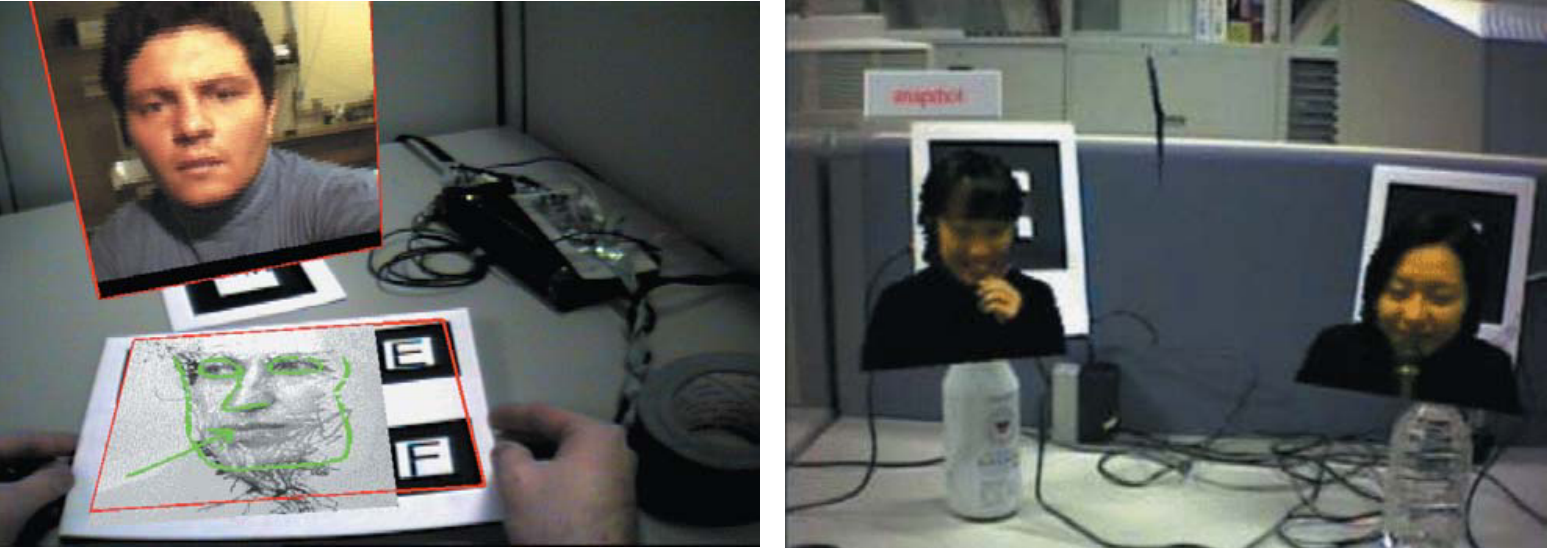
\includegraphics[width=\linewidth]{images/Billinghurst2002.PNG}
    \caption{Live virtual video avatars for remote collaborative AR interfaces. \cite{Billinghurst2002}}
    \label{fig:Billinghurst2002}
\end{figure}

\textcite{Muller2017} introduced adding shared virtual markers to help remote collaboration to be more effective and to understand the context of the collaboration. They found that the communication behaviour was improved and ambiguity was reduced in addition to an enhanced user experience. 

\section{Telepresence}      % why telepresence is relevant here

When people connect in this way, they may also want to share different amounts of information about their surroundings with each other. For example, users who are close friends in a social network may be happy to share a 3D virtual view of their surroundings and have the remote user appear as an AR avatar in their real space, while those that are strangers may only want to have an audio connection and not show anything of their surroundings to preserve their privacy \cite{Oetzel2011}. 

\textcite{Fuchs2014} (Figure \ref{fig:Fuchs2014}) studied telepresence via a scanned 3D environment to enable social connections with people and simulated face-to-face interactions. The remote person was scanned and reconstructed live in the local environment. They forecasted that 3D telepresence was going to be more popular when technology becomes more capable.

\begin{figure}
    \centering
    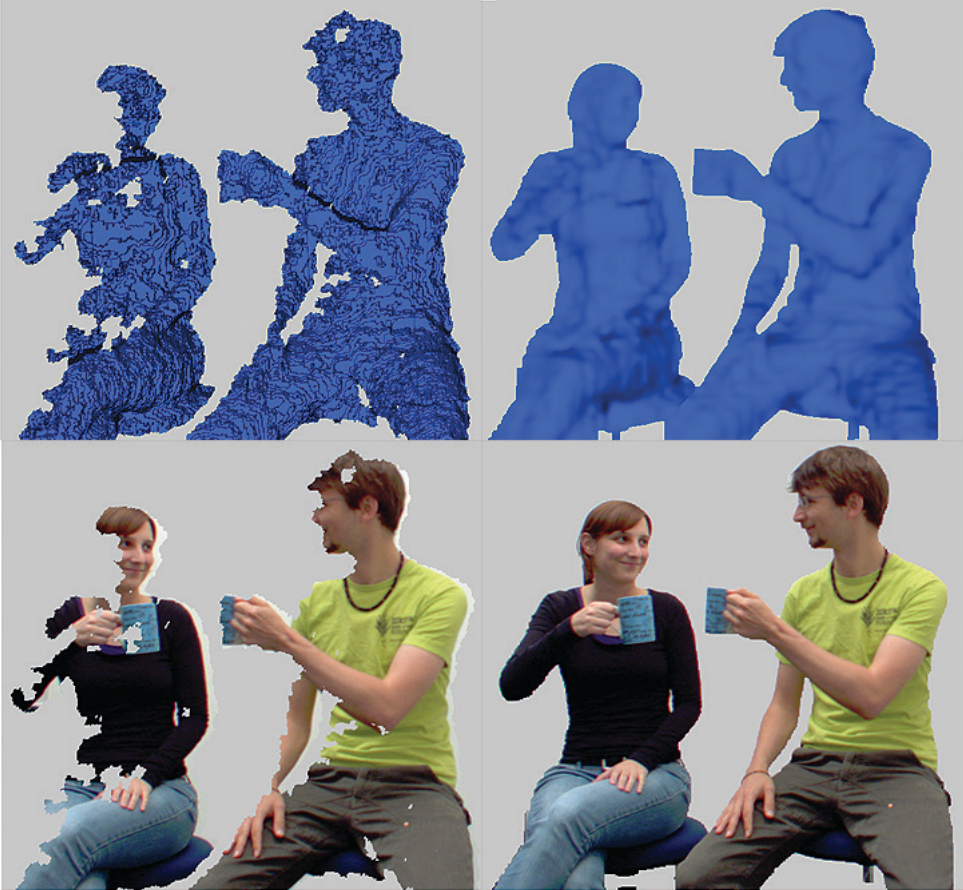
\includegraphics[width=0.8\linewidth]{images/Fuchs2014.PNG}
    \caption{Real-time 3D reconstruction of human \cite{Fuchs2014}}
    \label{fig:Fuchs2014}
\end{figure}

\section{Social Networks}

AR was used to enhance social presence and create more engaging experiences in video-based communications \cite{Almeida2012}. They built a prototype to segment the hand and overlay it on the video stream to create shared space experiences.

A lot of previous work looked into social interactions in AR \cite{Schmalstieg_144, Xu2008, Xu2011, Faas2010}. \textcite{Schmalstieg_144} built a hand-held game to test social interactions between players and found that mobility gives an advantage of making the game socially enjoyable and engaging. \textcite{Xu2011} reported on social interaction observation on a tabletop board game. The game is played through hand-held AR devices. They discovered five categories of social interactions: 1) chores, 2) reflecting on gameplay, 3) deciding strategy of play, 4) game itself and 5) out of game subjects. They found that chore-based social interactions are richer interactions and help the users to be more emotionally connected, which increases the engagement throughout the game.

Advancements in mobile phone hardware and increased network connectivity made live video streaming apps popular among smartphone users \cite{Liu2008}. Live video streaming apps have been used for sharing social experiences in various contexts. For instance, a person attending a conference or a concert could use their mobile phone to stream the event to their friends and family who could not be there. Similarly, live video streaming apps have also been used for social journalism \cite{Lenzner2014}, turning laypersons into live reporters. Consequently, these apps are now available from different sources with applications such as Periscope\footnote{https://www.periscope.tv/} and Facebook Live\footnote{https://live.fb.com/} among the most popular. These apps allow the users who are sharing to receive comments on the video they are sharing and to receive simple graphical feedback. 

Common features of live-streaming apps include as using the phones' camera which can be either pointed outward (recording what the user sees) or inward (where the user appears in the video), allow users to send a live video stream of what they are doing to hundreds or even thousands of viewers. The purpose of sharing the video is social, so the experience is improved if the viewer can also provide feedback.

\begin{figure}
    \centering
    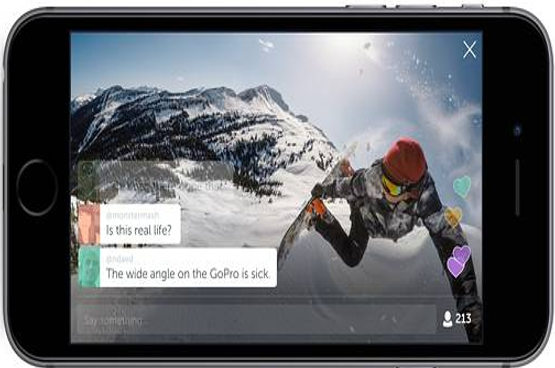
\includegraphics[width=0.4\linewidth]{images/periscope.png}
    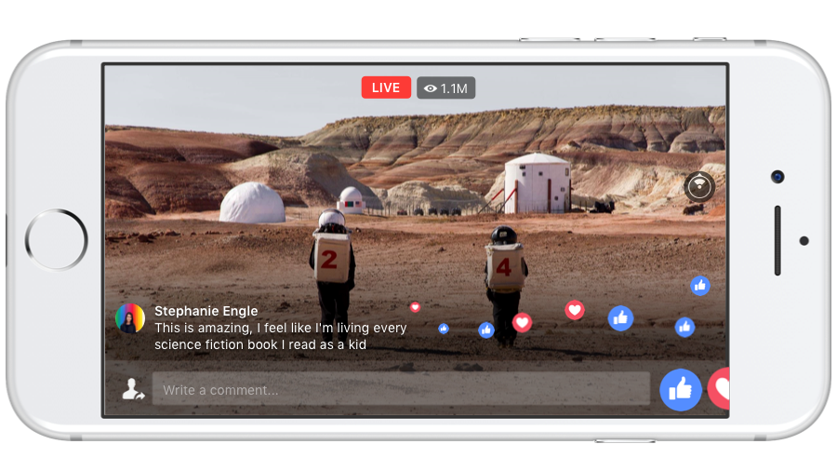
\includegraphics[width=0.4\linewidth]{images/facebook-live.png}
    \caption{Examples of live-streaming apps: Periscope (left) and Facebook Live (right). Note the user interface of comments from viewers are displayed as a list on the UI.}
    \label{fig:live-streaming}
\end{figure}

In these applications, the feedback comments usually appear in a list below or beside the video being shared (Figure \ref{fig:live-streaming}), separate from the visual context of what the viewer is commenting on. This may cause problems when the person sending the video changes their viewpoint. For example, a viewer might send the comment "I like that view", but by the time the comment appears, the view might already have changed from the view being commented on.

Future social interactions with wearable AR can be extrapolated from current social network interactions where friends share content and interact with others' content on mobile platforms such as Facebook and Instagram. For example, Facebook live allows a person with a mobile phone to live stream to remote collaborators. Similarly, wearable AR systems have already been developed that enable people to share a view of their surroundings. For example, the Shared Sphere work of \cite{lee2017mixed} allows a user with a wearable AR display to live-stream a 360-degree video of their surroundings to a remote collaborator, although only between pairs of users. 

\section{Social Proximity}

For representing "people" in AR space, \cite{Sousa2016} (Figure \ref{fig:Sousa2016}) studied the concept of \enquote{personal space} and \enquote{social bubbles} in terms of proxemic interactions between people in different places. They used floor projections and hand-held devices to communicate the presence of remote people. They also established a \enquote{gradual engagement model for remote proxemics} based on distance from the user, which consisted of 1) personal, 2) engaged, 3) peripheral and 4) ambient.

\begin{figure}
    \centering
    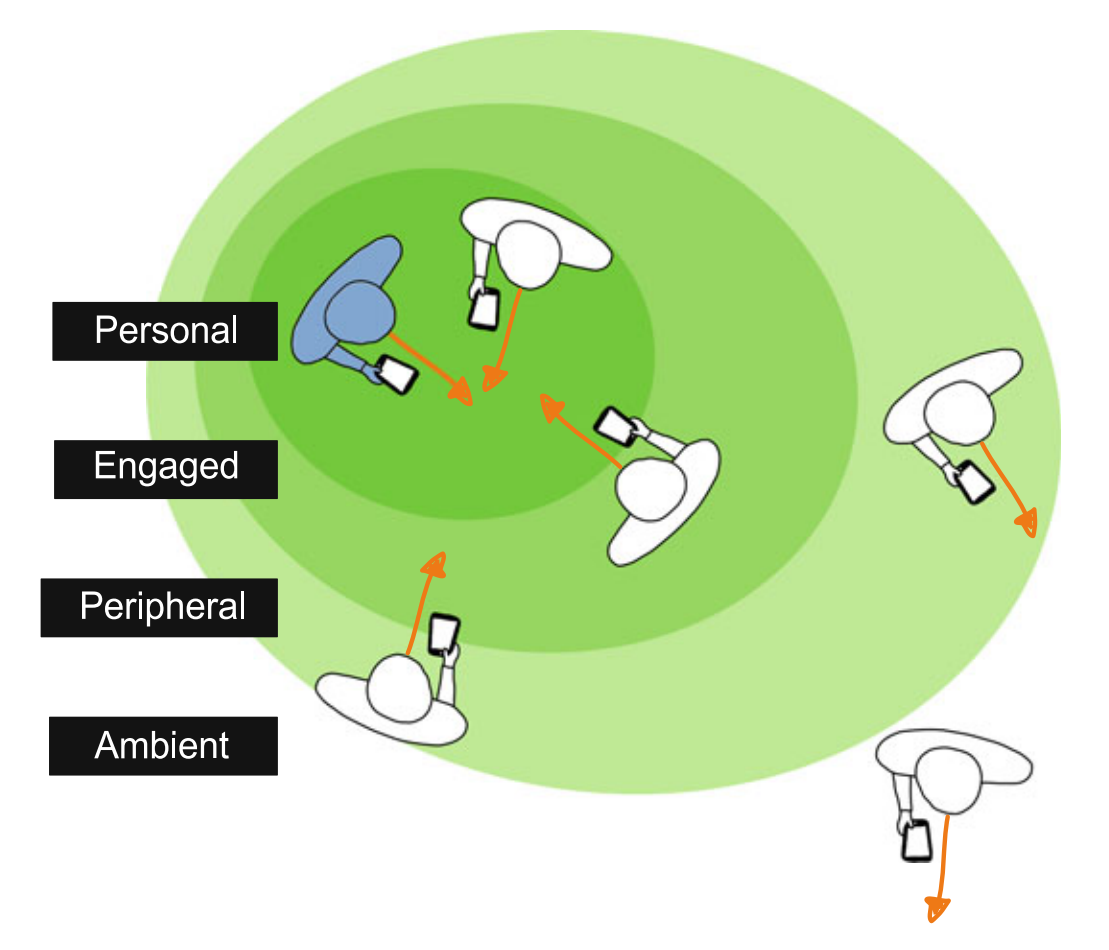
\includegraphics[width=0.8\linewidth]{images/Sousa2016.PNG}
    \caption{Gradual engagement model for remote proxemics representing four levels: 1) personal, 2) engaged, 3) peripheral and 4) ambient. \cite{Sousa2016}}
    \label{fig:Sousa2016}
\end{figure}

\textcite{Leshed2012} studied different representation of social relationship and identity in second life, and found that people use metaphores such as onion layers to represent layers of their identity gradually revealing as the interpersonal relationship developed between people. 

\cite{Gergle2004}


Most previous work has focused on how visual representation and proximity could be used to organise an AR representation of a person's social network. However, this information could also be used to modify the contextual information being shared by a user out to their social network as well. 

\section{Virtual Avatars}

In the social AR/VR space, previous work implemented a variety of visual representations of self and others. \textcite{Fanello2016} prototyped live sharing of a full scan of a person's body with remote users using 3D cameras and the HoloLens\footnote{https://www.microsoft.com/en-nz/hololens}. 

Scaning a person body in 3D has become more accessible to consumer scale. For instance, Echo Look by Amazon\footnote{https://en.wikipedia.org/wiki/Amazon_Echo#Echo_Look} is a 3D depth camera that people can use pose in front of the camera and use AR to overlay different outfits on themselves to see how they would look before purchasing the outfit. The person can share their photo with few outfits with their friends to get feedback on which outfit would look better. 

Similarly, some companies (such as High Fidelity\footnote{https://highfidelity.com/}, Sansar\footnote{https://www.sansar.com/}, Itsme3D\footnote{https://www.itsme3d.com/}) and other VR shared worlds) are building social VR experiences in which users are represented as 3D virtual avatars. In the social VR space, previous work implemented a variety of visual representations of self and others. For instance, virtual avatars have been used to share social experiences such as in Facebook Spaces\footnote{https://www.facebook.com/spaces} (Figure \ref{fig:facebook-spaces}) where users can meet in VR, take selfies and teleport to a 360-degree video. Virtual avatars for self and others are represented as a floating face and upper body rendered in a VR background. 

360 videos have been studied as a medium for mixed reality enabled remote collaboration tasks \cite{Tang2017a, Lee2017, lee2017mixed, Lee2019}. Results show that by using 360 videos, the remote user can have an independent view of the local person and be able to achieve higher co-presence and more effective in task completion. 

\begin{figure}
    \centering
    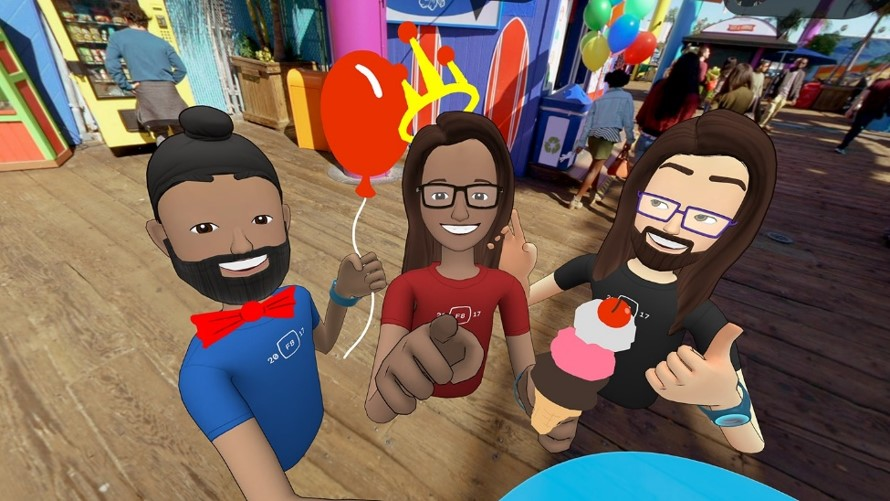
\includegraphics[width=0.8\linewidth]{images/facebook-spaces.jpg}
    % 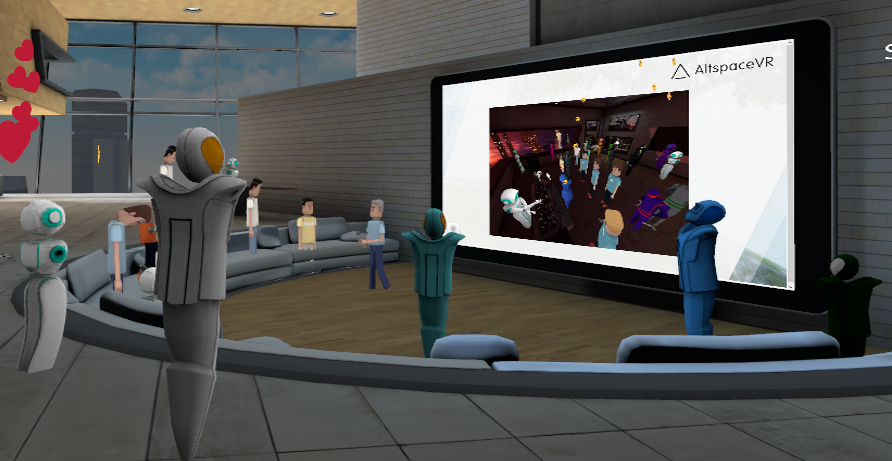
\includegraphics[width=0.4\linewidth]{images/altspace-vr.png}
    \caption{Example of avatars in VR. Facebook Spaces}
    \label{fig:facebook-spaces}
\end{figure}

As for the social AR spaces, there have been limited examples of social applications. Avatar Chat was introduced by Magic Leap\footnote{https://www.magicleap.com/experiences/social} (Figure \ref{fig:ml-avatar-chat}) in late 2018. The app allows users to connect with their social contacts and view their avatar overlaid on top of their physical environment. Users can share emojis, connect to a group "avatar" chat and talk about images overlaid in their space. The avatars are cartoonish-looking representing the upper half of the body floating in the AR space. Natural hand gestures are detected using the depth cameras on the device, assisted by computer vision algorithms and translated to a pre-defined set of virtual hand gestures to the other participants in the chat session. 

Saptiate\footnote{http://spatiate.com/} is another social app launched in early 2019 on Magic Leap where users can connect in a chat session with primitive avatars, sketch in their AR world, and share the sketching in real time with connected users. The users can see each other's avatars and hear their voices. 

\begin{figure}
    \centering
    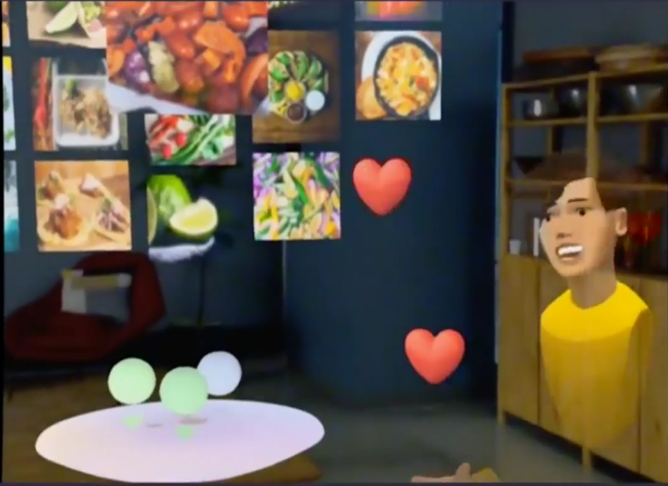
\includegraphics[width=0.8\linewidth]{images/avatar-chat-1.png}
    % 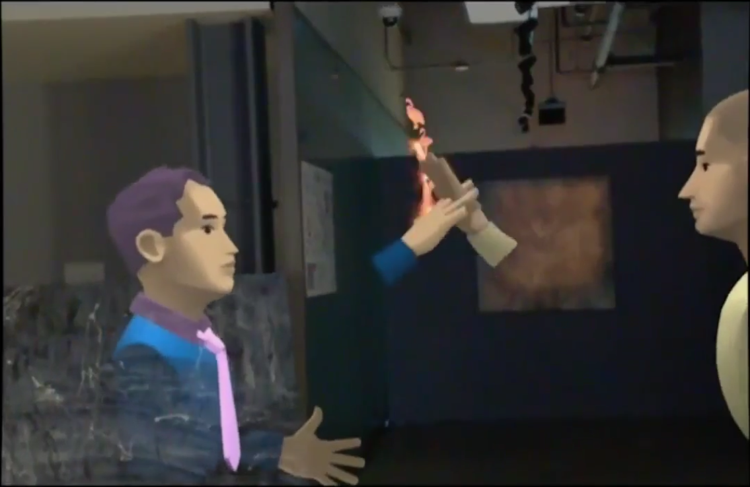
\includegraphics[width=0.4\linewidth]{images/avatar-chat-2.png}
    \caption{Example of avatars in AR - Avatar Chat by Magic Leap}
    \label{fig:ml-avatar-chat}
\end{figure}

However, representing social contacts in VR/AR can be cumbersome. It will be more cluttered and overwhelming to represent the data content that social avatars are trying to share. Representing futuristic concept videos have imagined social data (e.g., "Hyper Reality"\footnote{https://www.youtube.com/watch?v=YJg02ivYzSs} and "Merger"\footnote{https://www.youtube.com/watch?v=SqW2dEkiD-Y}) where social data can clutter the AR view of the user. It will also raise privacy and ethical concerns.

\textcite{Greenwald2017} - studied social presence in room scale VR. They used virtual avatars for communicating and collaboration in a social setting. They found that using embodied avatars in VR interactions is practical for collaboration tasks with the benefit of social presence. One of the tasks was drawing to communicate, which was challenging for participants. 

\textcite{Jo2016} studied the influence on co-presence of the background environment (AR vs VR) and the fidelity of the avatar representation of the remote user (photo-realistic vs pre-built). They found that more realistic avatars had a positive impact on the feeling of co-presence between remote collaborators. \textcite{Volante2016} also studied the impact of the visual appearance of avatars (realistic vs. stylised) on the inter-personal emotional response of participants. They also found that more visual realism has lower adverse effects on the PANAS scale, which measure the intensity of the emotion at a given time. Researchers have been investigating the social aspects of multi-user VR environments. \textcite{Ducheneaut2006} studied massive multiplayer online games in terms of social activities, and found that while users may prefer to be with other players, they do not necessarily like actively interacting with them. This led us to think that users may want to have the sense of the presence of social contacts around them, but not necessarily interact with them.

\textcite{Harris2009} studied the social behaviour of users of Second Life\footnote{secondlife.com} and found that users became less active over time and go to familiar places rather than being explorative and actively teleporting/flying. They found out that people prefer routine and to be surrounded by familiar faces/places over time, forming a social group.

% mark: [you should about how they handle crowds or if everyone is just represented the same] 
However, there has been very little research into social representation in AR. The AR space is more challenging in terms of finding the best locations to fit avatars in the real world so they do not interfere with physical objects or appear suspended in mid-air. However, a social AR application can also allow people to see their friends while doing other tasks; users do not have to use an immersive VR environment to see their social contacts.

Researchers have also explored different ways of managing a large number of information tags in AR interfaces. \textcite{Julier2002} showed how environmental cues, such as distance and user context, can be used to filter AR content into the most relevant information. \textcite{Hollerer2001} describe how can the view management techniques be used to ensure that virtual objects can be easily seen in collaborative AR interfaces. Similarly, \textcite{Grasset2012} show how an image-based approach can be used to ensure AR information tags do not overlap in hand-held AR. 

This previous research shows that visual fidelity can be used to distinguish between virtual avatars. Different visual representations and spatial cues can also be used to distinguish between information tags in an AR interface. However, there has been little or no research on how to manage social network representations in AR for large numbers of connections. The next section explores how visual and proximity cues could be used to organise contacts in a wearable social AR interface.

% \todo[inline]{[In this section you should probably also mention how VR Virtual Avatar environments handle hundreds or more simultaneous users. For example, what tools does second life have for connecting people to hundreds of others. This is directly relevant to your thesis topic]}


%----------------------------------------------------------------------------------------
%    Summary
%----------------------------------------------------------------------------------------
\section{Summary}

This work aims to layout the space of the Social AR Continuum for social sharing experiences by looking at parameters and options that can be changed in terms of people, objects and the environment to create a shared AR experience. 

Building on previous work on proximity-based relationships \cite{Sousa2016}, this work focuses on the shared contents of social avatars in an asynchronous situation. Unlike previous work on social avatars, this thesis studies representing social contacts in a large-scale network. The aim of this work is to reduce the clutter that may be caused by displaying the social avatars and their shared content. This thesis addresses the question of how we can use the social relationship between avatars and the viewer as a way to filter and enhance viewing the shared-content experiences. 

The scope of this thesis is to explore options of visual user experience design in social AR, including displaying contacts, displaying shared data, and displaying shared environments. This thesis does not necessarily cover all possible experiences but highlights the main points of interactions and reports on user studies measuring the sense of presence and privacy concerns that may occur from these experiences. 

The summary of the trends in the past work is that
% summary of wearable AR 
wearable AR has been the target of many previous developments and research directions. Aiming to enable true outdoor experiences and to be untethered to physical places would allow more exploration of the surrounding world. 
% summary of AR collaboration 
Most of the previous work on AR was focused on AR applications for remote collaboration and expert-helper situations. Very few focused on how AR is used in connecting with our friends and family and for sharing social experiences.
% Summary of social AR
In the social aspects of AR, previous work showed few attempts of representing social networks in AR and VR. Also, some applications looked into scanning and using human avatar representations for social connections with others.

The limitation of past work is that it was mainly focused on the remote collaboration of local worker/remote helper situations. However, it did not address sharing social experiences with friends and family scenarios. There is some new work in this area, but not enough to cover all dimensions in this field. The gap that this thesis is addressing is the user interaction design of future wearable AR interfaces so that it can be easily used for sharing social experiences with family and friends. 

This thesis is important because it explores different ways of presenting social networks on wearable AR and helps application designers and developers by providing insights into building similar applications that have a higher chance of being effective and acceptable to users. 

The contributions to the current state-of-the-art are: 1) building software prototypes of sharing social experiences on wearable AR platforms, 2) Running user studies on these prototypes and analysing the results, 3) providing the foundations of the design space of sharing social experiences on wearable AR. 

% \todo[inline]{Gun: You should have a paragraph summarising the trend in the past work and what is the limitation to support why your work is important. Or you may add a section at the end of this chapter that does an overall review of the whole chapter and describe how your thesis makes contribution to the current state-of-the-art.}

% \todo[inline]{You should end the chapter with a summary of the research gap that you're going to be addressing.}

% \todo[inline]{[At the end of the related work section you should have a sub-section that provides a summary of the research, particularly highlighting the research gaps and shortcomings of this earlier work. You can then talk about which aspects that you are going to explore further in your PhD thesis. Highlight what is the novelty of your thesis, and what will be the main contributions that your research will make, relative to the earlier related work] }

% \subsection{Sharing for Collaboration}
% \subsection{Sharing for Social}


\chapter{The Social AR Continuum}
\label{ch:continuum}

This chapter describes The Social AR Continuum, a space for shared social experiences using wearable AR. It explores various dimensions, discusses options for each dimension, and outlines possible scenarios where these options might be useful.

Mixed and Augmented Reality allows us to visualise information in place. This information can have a specific relationship with that place (e.g., textual labels providing additional information with respect to the place) but their relation can also be that the place is just a good "position" to visualise this information (e.g., a physical wall in a room being a good position to visualise/augment pictorial information that has otherwise no immediate connection to this wall). In particular, the latter can also be used to visualise information created within the social networks of the user. This is of relevance because social networks (private and professional) are nowadays probably one of the most significant data sources/content generators for digital information. Given the sheer amount of information, intuitive and useful visualisation of this information may support the user when AR interfaces are more ubiquitous. Special care has to be taken when visualising information, not only on where to place it but also on how to visualise the information. Besides the question of where to place the digital information, a key question is also how this information can be represented depending on the social proximity between the users and their social graph. This is the motivation for defining a continuum that identifies the main dimensions that can be manipulated when exploring the sharing of experiences and information using an AR interface. 

This work categorises the social AR dimensions into three areas: 
\begin{enumerate}
    \item People (self and others),
    \item Data (including virtual objects and the surrounding environment), and
    \item Interactions between people and data (including annotation)
\end{enumerate}

Representing self and others as avatars is described in more detail in Chapter \ref{ch:contacts}. The surrounding environment and sharing different types of data are described in more detail in Chapter \ref{ch:data}, while the interactions between people, in the form of annotation of the surrounding environment, are described in Chapter \ref{ch:annotation}.

% Tobias: Again, this is just some sentences that just came out of my head. You can use or not use at your own risk and will. However, it has to be expanded (your story but also my draft above) as there is way more to say about. At occasions, you will have the feeling that you will repeat things that you mentioned earlier (e.g. introduction and related work). That is normal, and the repeating of information is often needed for the reader to follow your motivation and argumentation. Remember: Your reviewers are likely reading your thesis late after work and will be tired. An occasional reminder of what this is all about will be appreciated as long as it is coherent and you do not start to contradict yourself.

% \begin{figure}[ht]
%     \centering
%     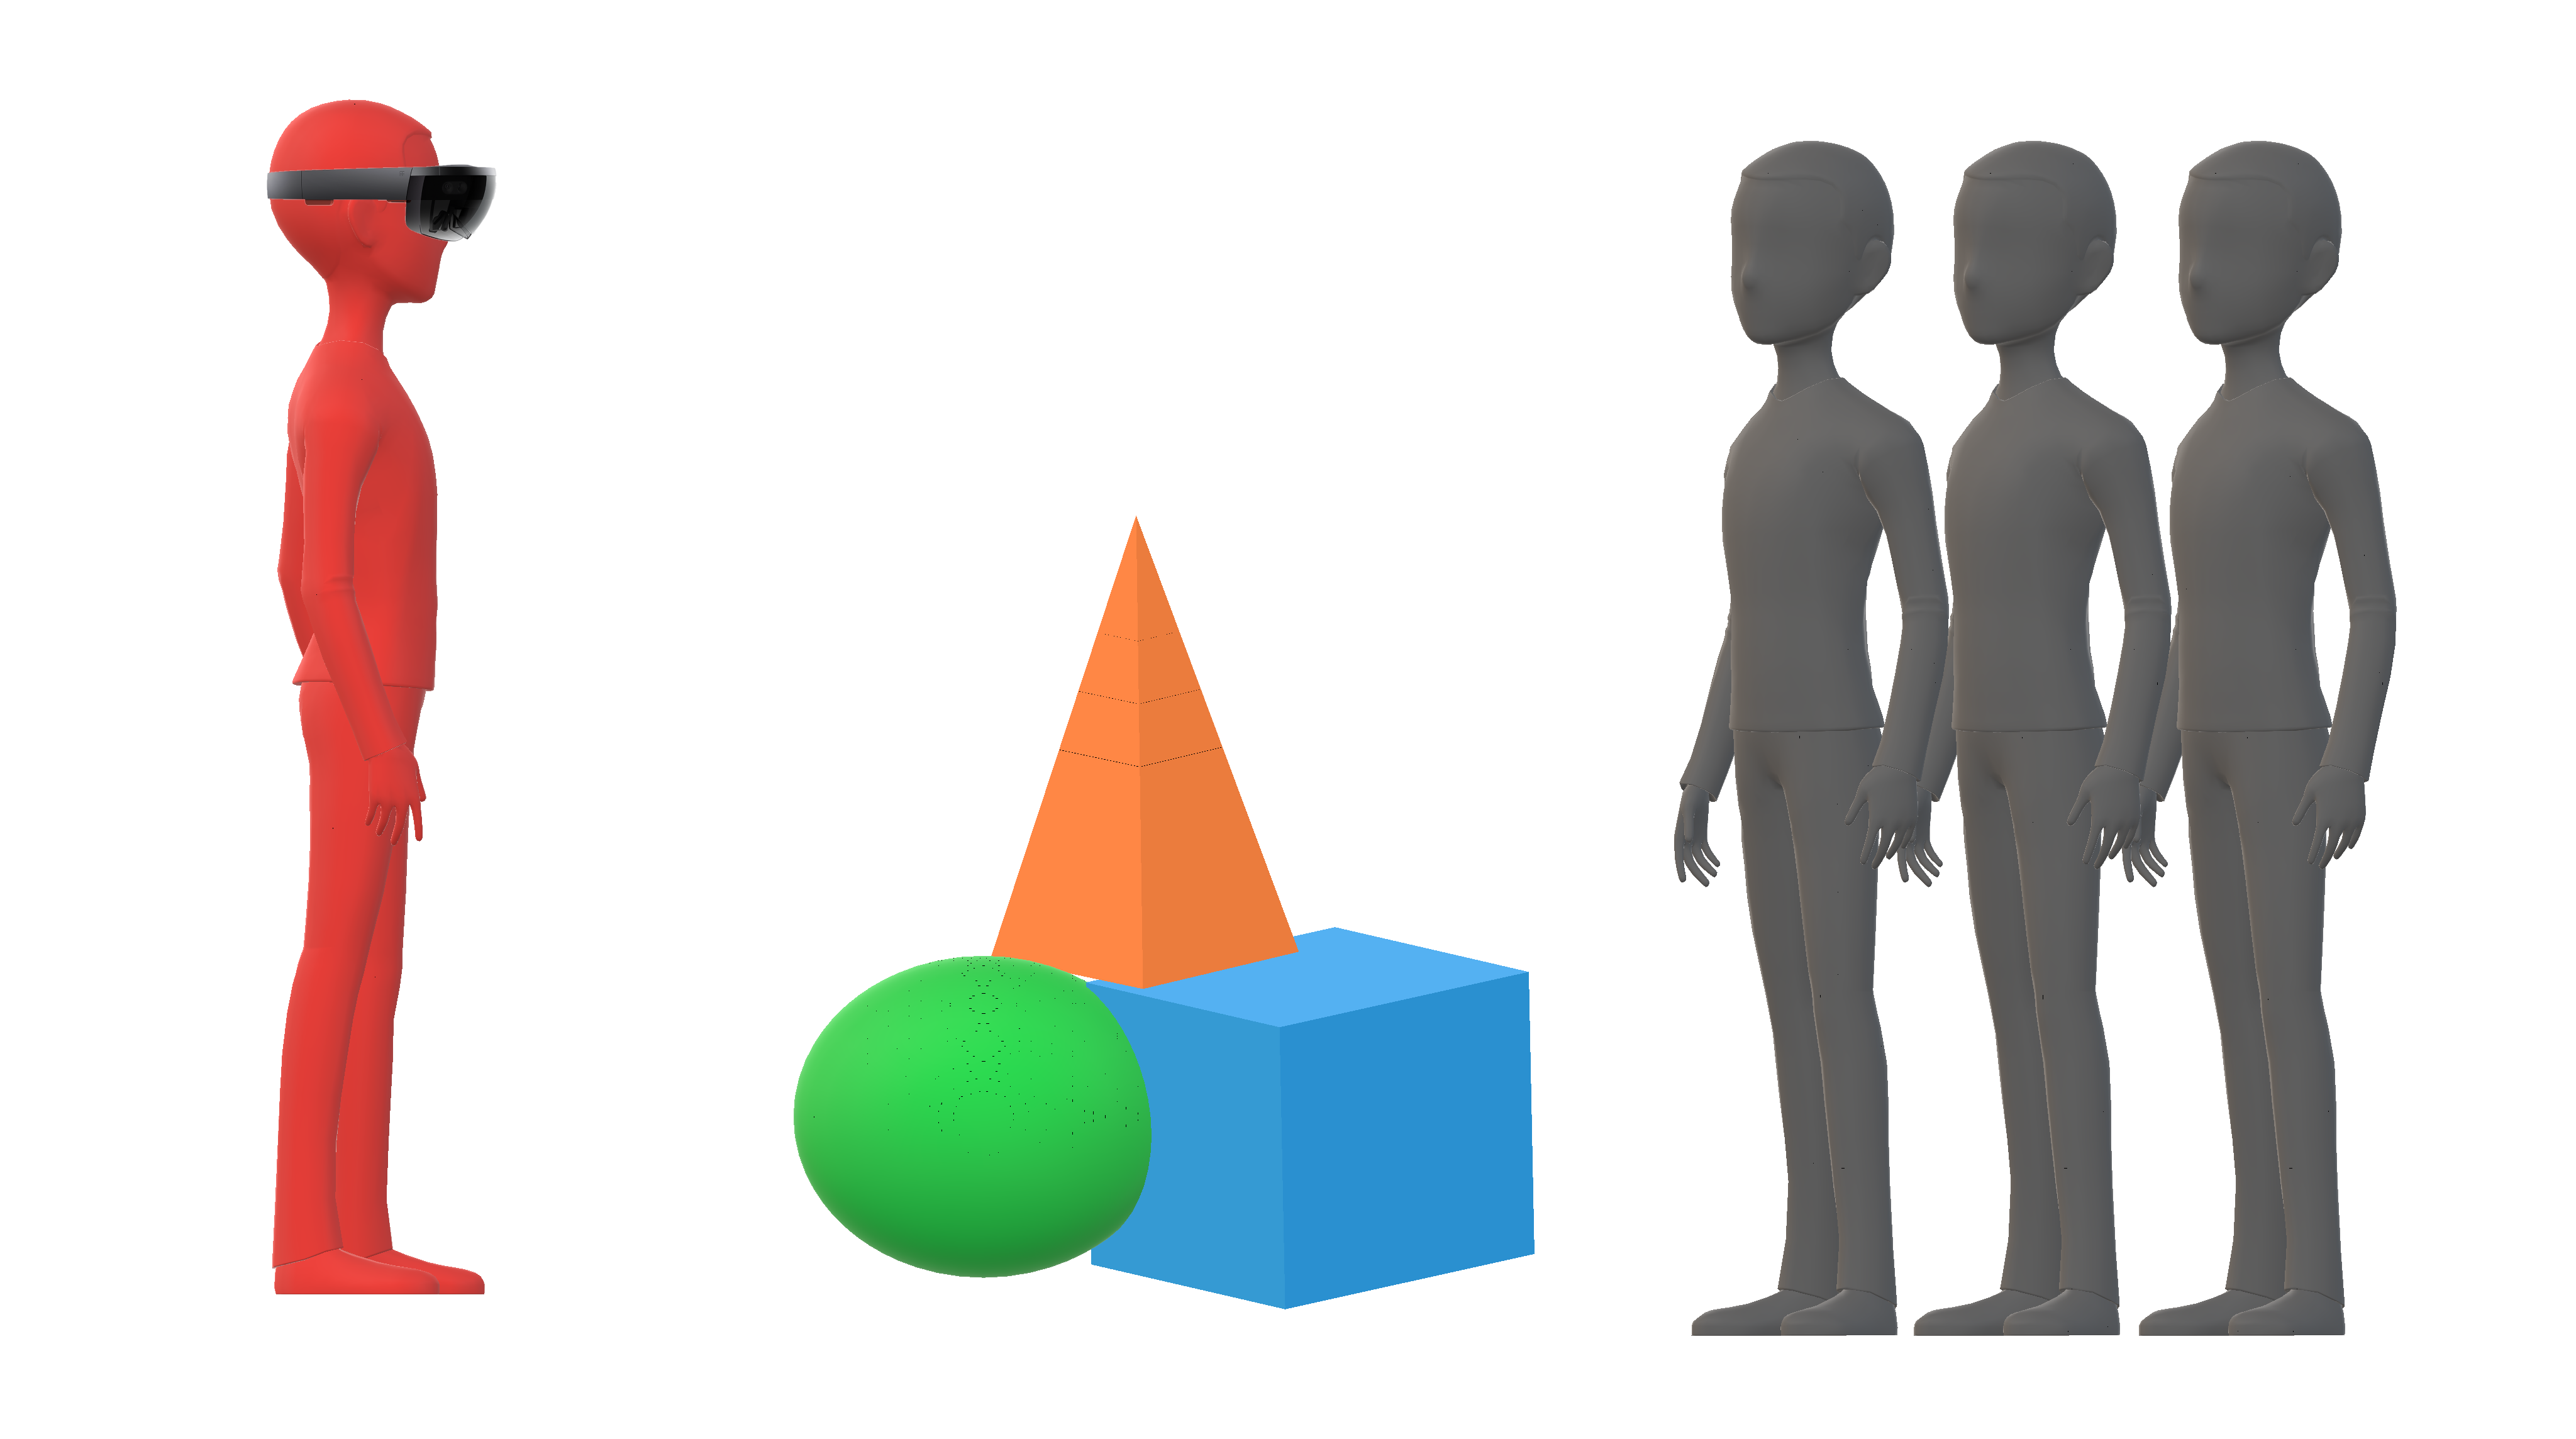
\includegraphics[width=0.8\linewidth]{images/30-continuum/continuum_categories5.png}
%     \caption{The Social AR Continuum categories: 1) People (self and others), 2) Objects (surrounding environment), 3) Interactions (e.g., annotations)}
%     \label{fig:continuum:categories}
% \end{figure}

This work aims to layout the space of the Social AR Continuum for social sharing experiences by looking at parameters and options that can be manipulated in terms of people, objects and interactions to create a shared social AR experience. Before diving into the parameters of shared social experiences, the next section explores potential future scenarios where people would want to share social experiences through AR.

\pagebreak
\section{Scenarios}
% \todo[inline]{explain all the things no just what is depicted in the picture…. later explain the other scenarios but similarly motivate for each scenario why this is a valid and important scenario.}

% Tobias: First of all I like graphics etc. I was even thinking if you should start with the scenarios before coming to the AR continuum. IIf you could use your scenarios to motivate the need for an AR continuum better?! Later, you can use them again to explain some of the dimensions. In any case, they are under-utilised at the moment. They need a better explanation and better integration. For example, I would not start with the decoration one because it is the weakest one in my opinion. Maybe better start with working from home and the social meeting. You could start with that  ….. blabla bla… explain all the things no just what is depicted in the picture…. later explain the other scenarios but similarly motivate for each scenario why this is a valid and essential scenario. 

% Again, these are all recommendations, and you can take it or leave it (or take parts of it). In any case, you need to integrate more references. I only put in the last part some examples on where they are needed, but basically, every big statement should be supported. I think this is all-important because when the reader is not buying in into your scenarios, you will have a hard time selling your conceptual solutions for each scenario. The reader will simply say: The scenario is not a real scenario or is to irrelevant to be addressed by a PhD thesis as it is not solving a real problem (current and future). This is a bit of the issue with the decoration scenario, which is a bit random. Keep it but do not put it first.

% Finally, please be more verbose in your figure captions. I have the tendency to be very long (see my PhD thesis and most of my papers) but really take the space to explain what is going on in the figure and do not only provide a "figure name". It is OK if parts are replicated in the body text. But the figure should work without the body text, and the body text should work without the figure caption.

Let us consider the following future scenarios of sharing social AR experiences:

\subsection{Working from home}

There is increasing support for working from home \cite{Bloom2015, Crosbie2004, Olson1984} and AR/MR could be a key technology here to connect remote teams and people \cite{Koehne2012, Maarouf2012}. However, when sharing information with remote parties, we should also consider their social proximity when deciding on what to share and how to share it. Let us consider the following example where user A is working from home and is using an AR system to share.

The user is working from home (Figure \ref{fig:illustration:group-meeting}) and sharing their surroundings with 1) a close colleague with a few messy objects hidden/blocked, 2) a colleague who sees a clean and tidy room with projection on the wall as additional augmentation, and 3) a group meeting with other workers where nothing is visible in the background. 

\begin{figure}[ht]
    \centering
    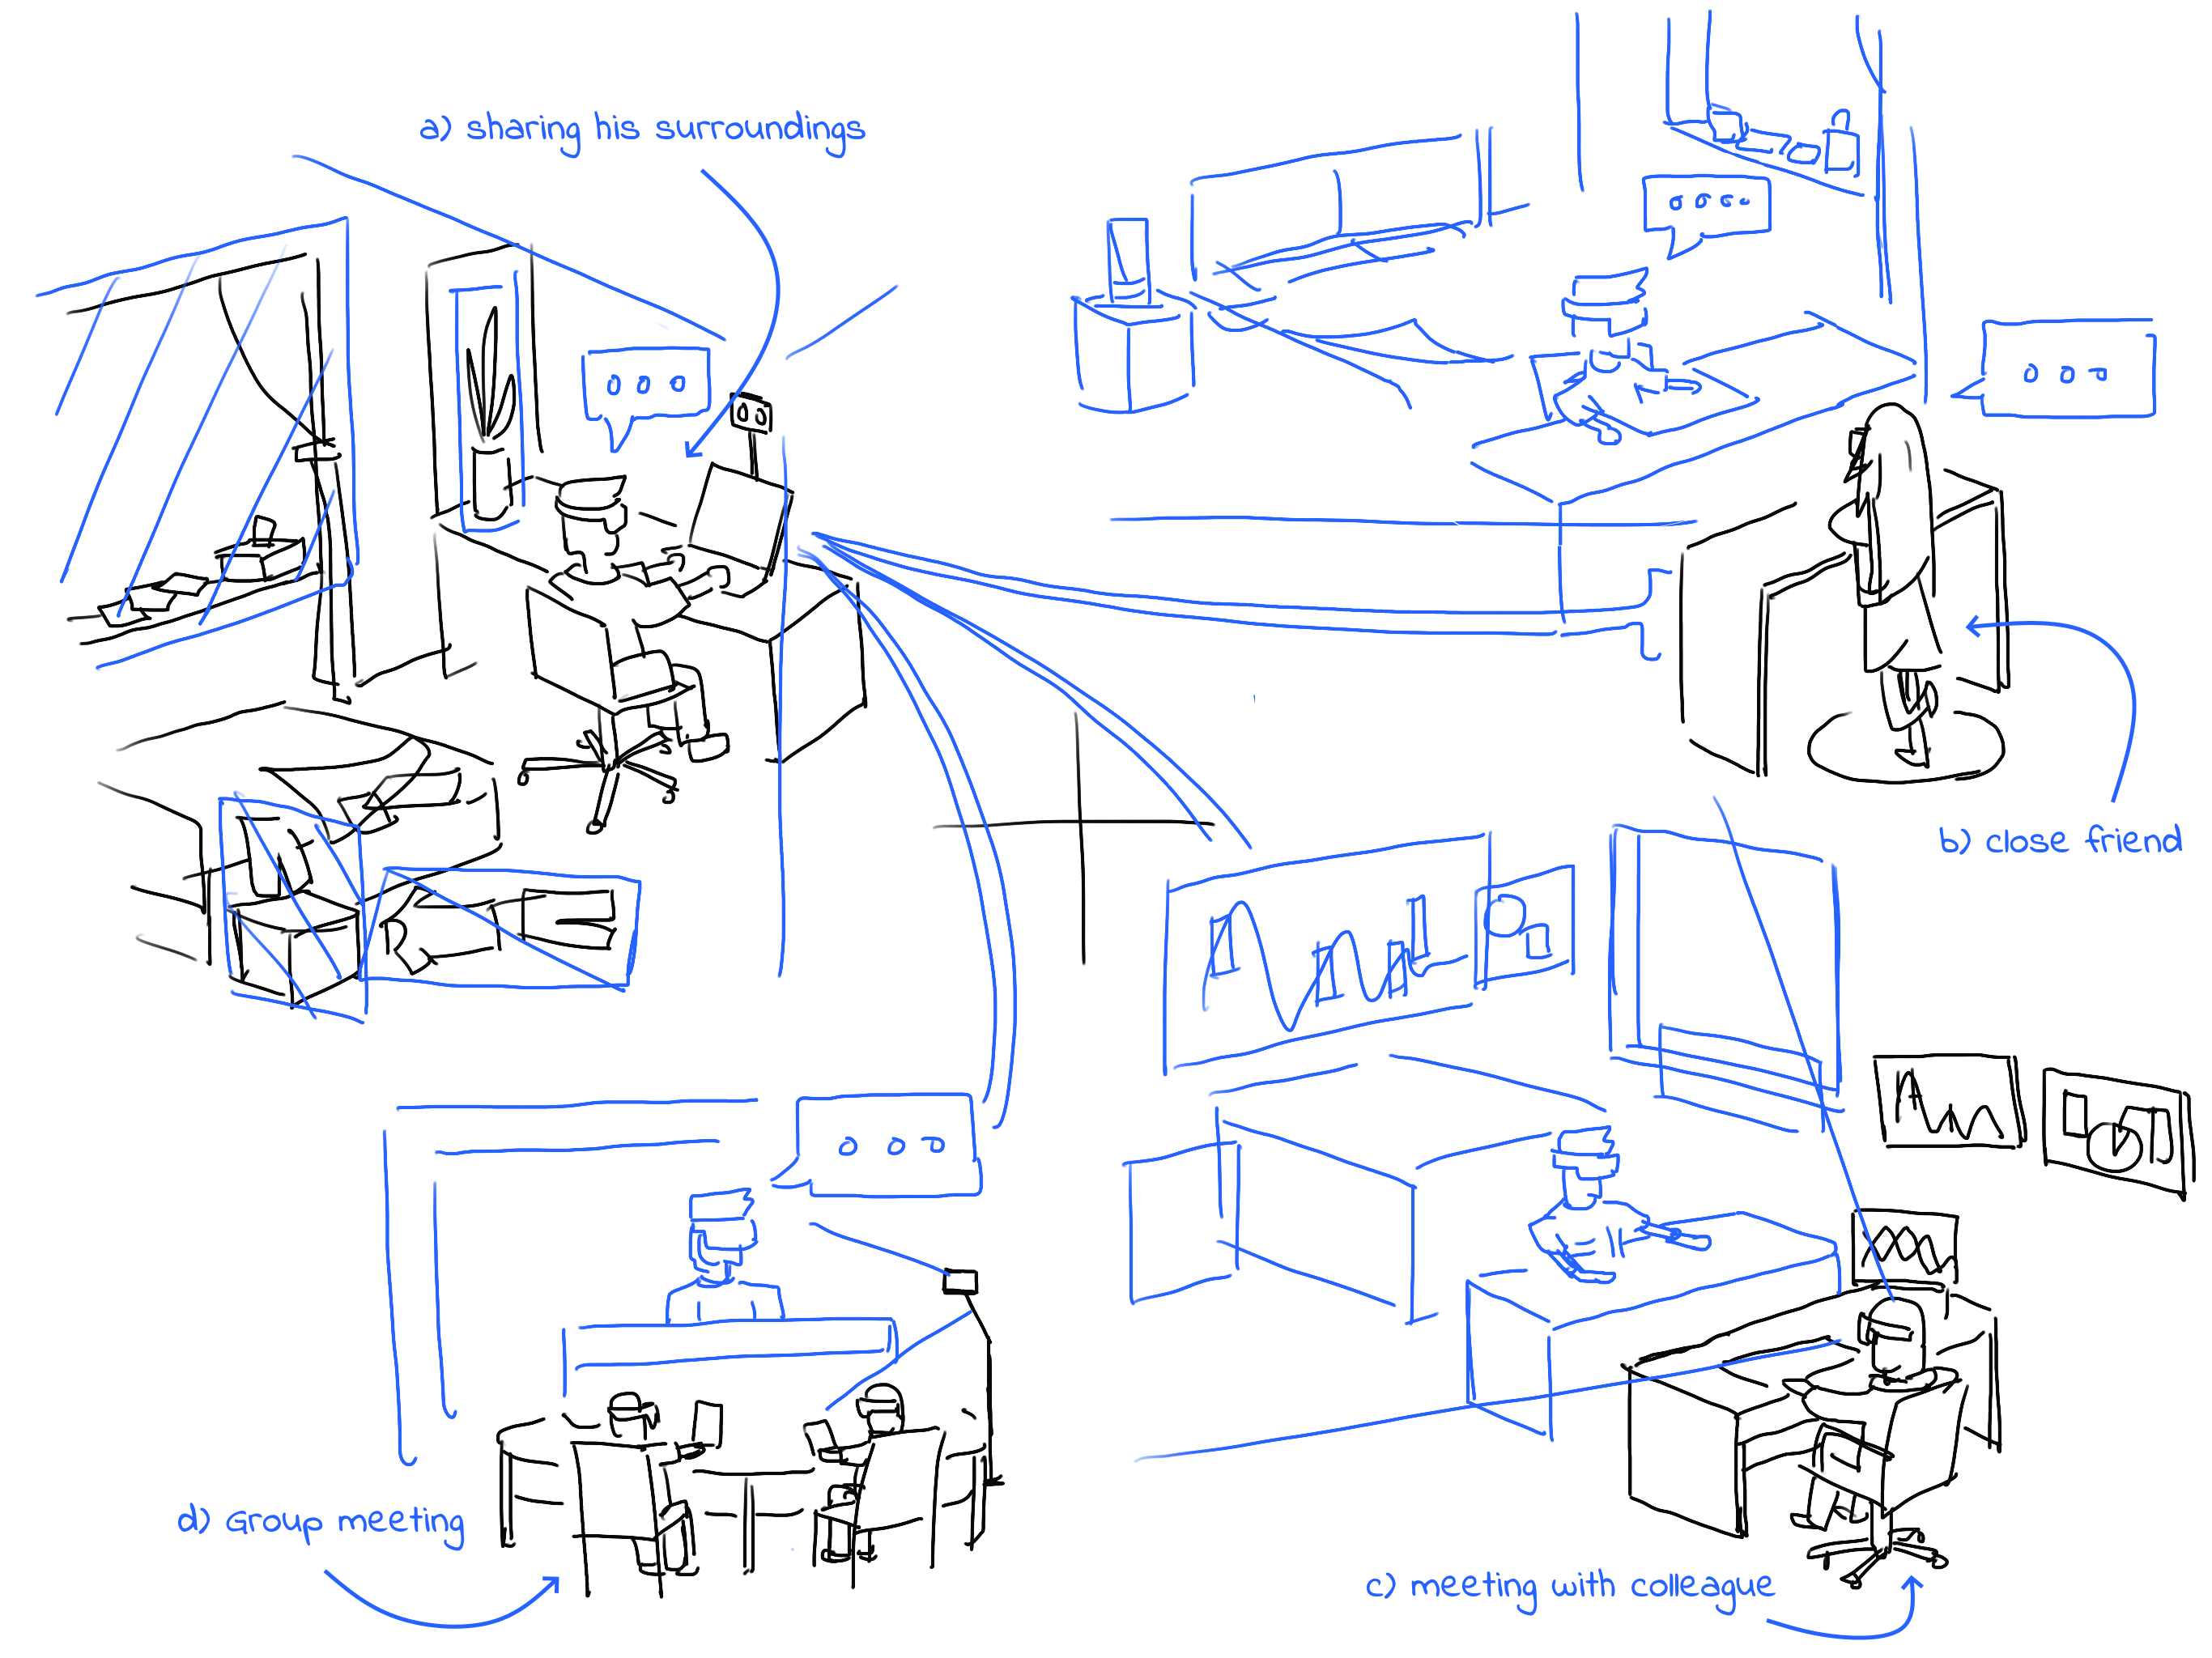
\includegraphics[width=\linewidth]{images/30-continuum/illustrations/2_Group_Meeting.png}
    \caption{Working from home scenario. The user (top left) is sharing his space with 3 different people; 1) a friend (top right) where she sees his background space tidy, 2) a co-worker (bottom right) where most things in the background are overlaid with a box hiding the details, and 3) a business group meeting (bottom left) where nothing is visible from his background.
    (Illustrated by Kris Tong)}
    \label{fig:illustration:group-meeting}
\end{figure}

\subsection{Conference}

The user is at a conference (Figure \ref{fig:illustration:conference}) and shares an idea that he is thinking about. However, because people around him are not close to him, they see low-fidelity details about these ideas (e.g., abstract and title). While networking with others, the user may choose to share more details about the idea with a particular person who is in a direct conversation with him and interested in further collaboration opportunities.

\begin{figure}[ht]
    \centering
    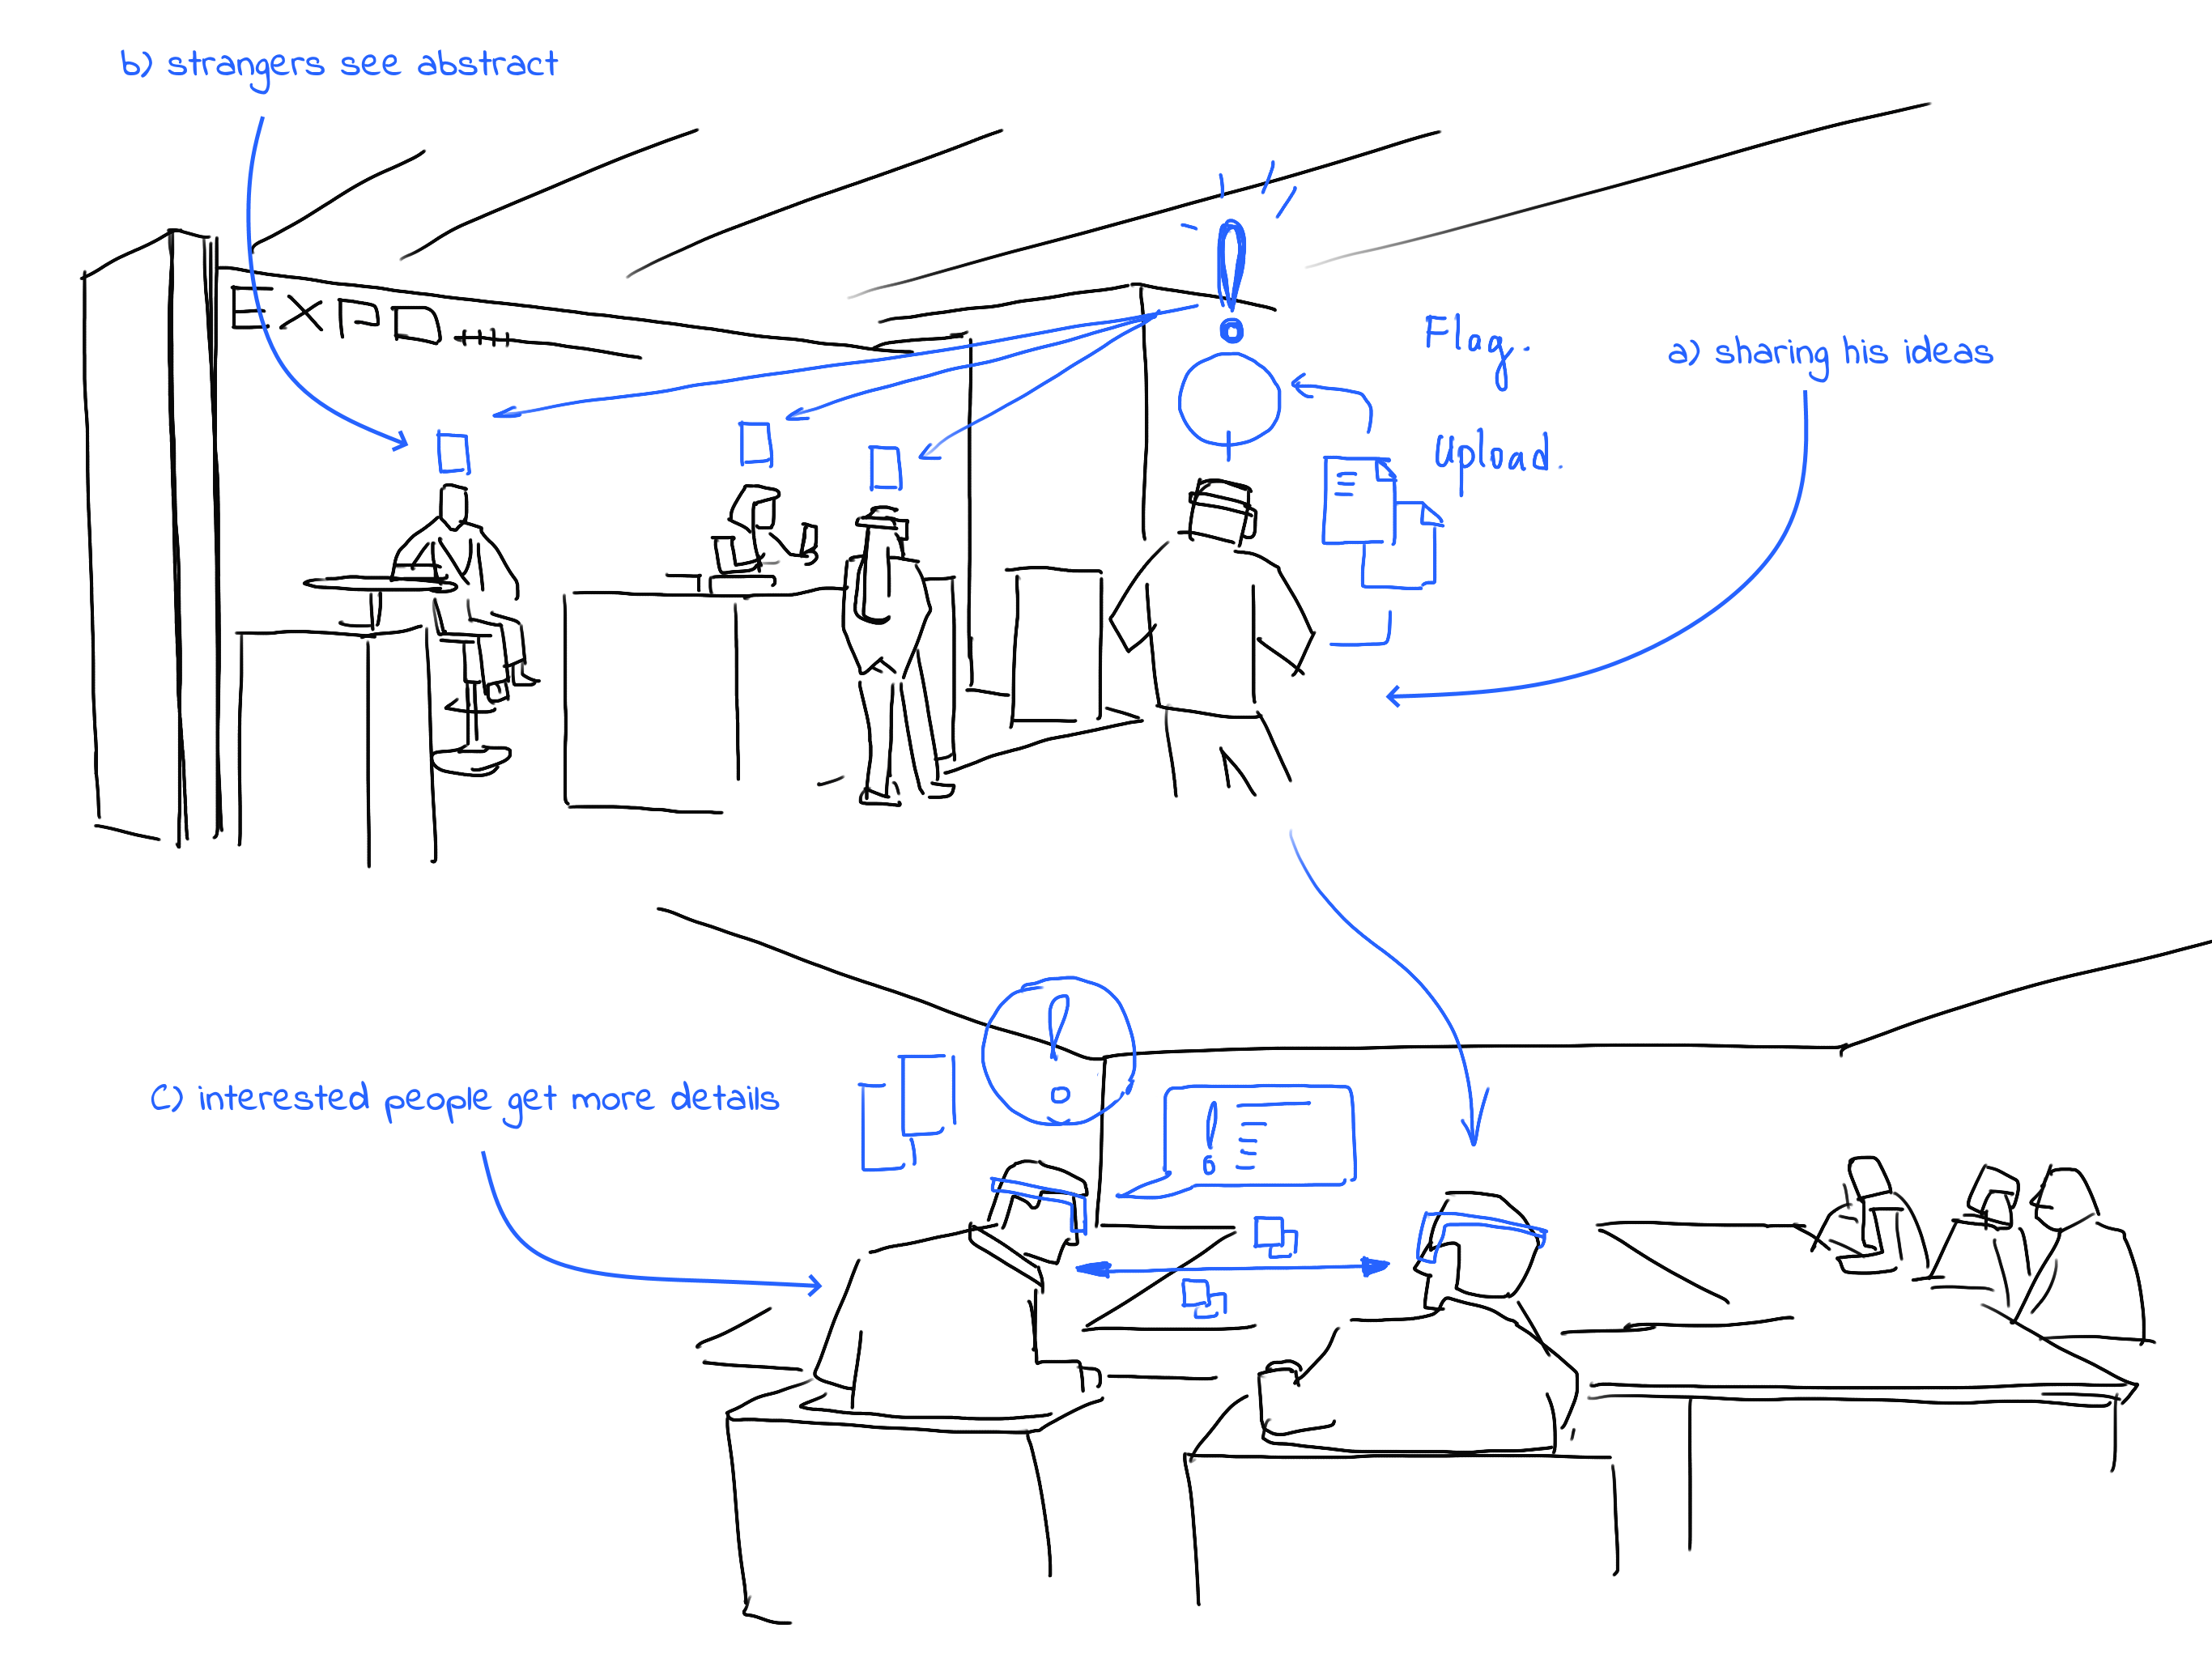
\includegraphics[width=0.8\linewidth]{images/30-continuum/illustrations/4_Flag_On_Conference.png}
    \caption{Conference scenario. The user (top) walks through a conference sharing his ideas about the conference topic in high-level with strangers. When he meets a like-minded person (bottom), he may share more details about these ideas with that person. (Illustrated by Kris Tong)}
    \label{fig:illustration:conference}
\end{figure}

\subsection{Social event}

The user is at a social event (Figure \ref{fig:illustration:social-event}), where he is meeting people face to face for a drink. He can see through their headset what their friends are sharing. For the close friends, he can see high-fidelity material such as 360-degree videos of their last trip, while for others who are less close to him, he sees low-fidelity media such as 2D images. 

\begin{figure}[ht]
    \centering
    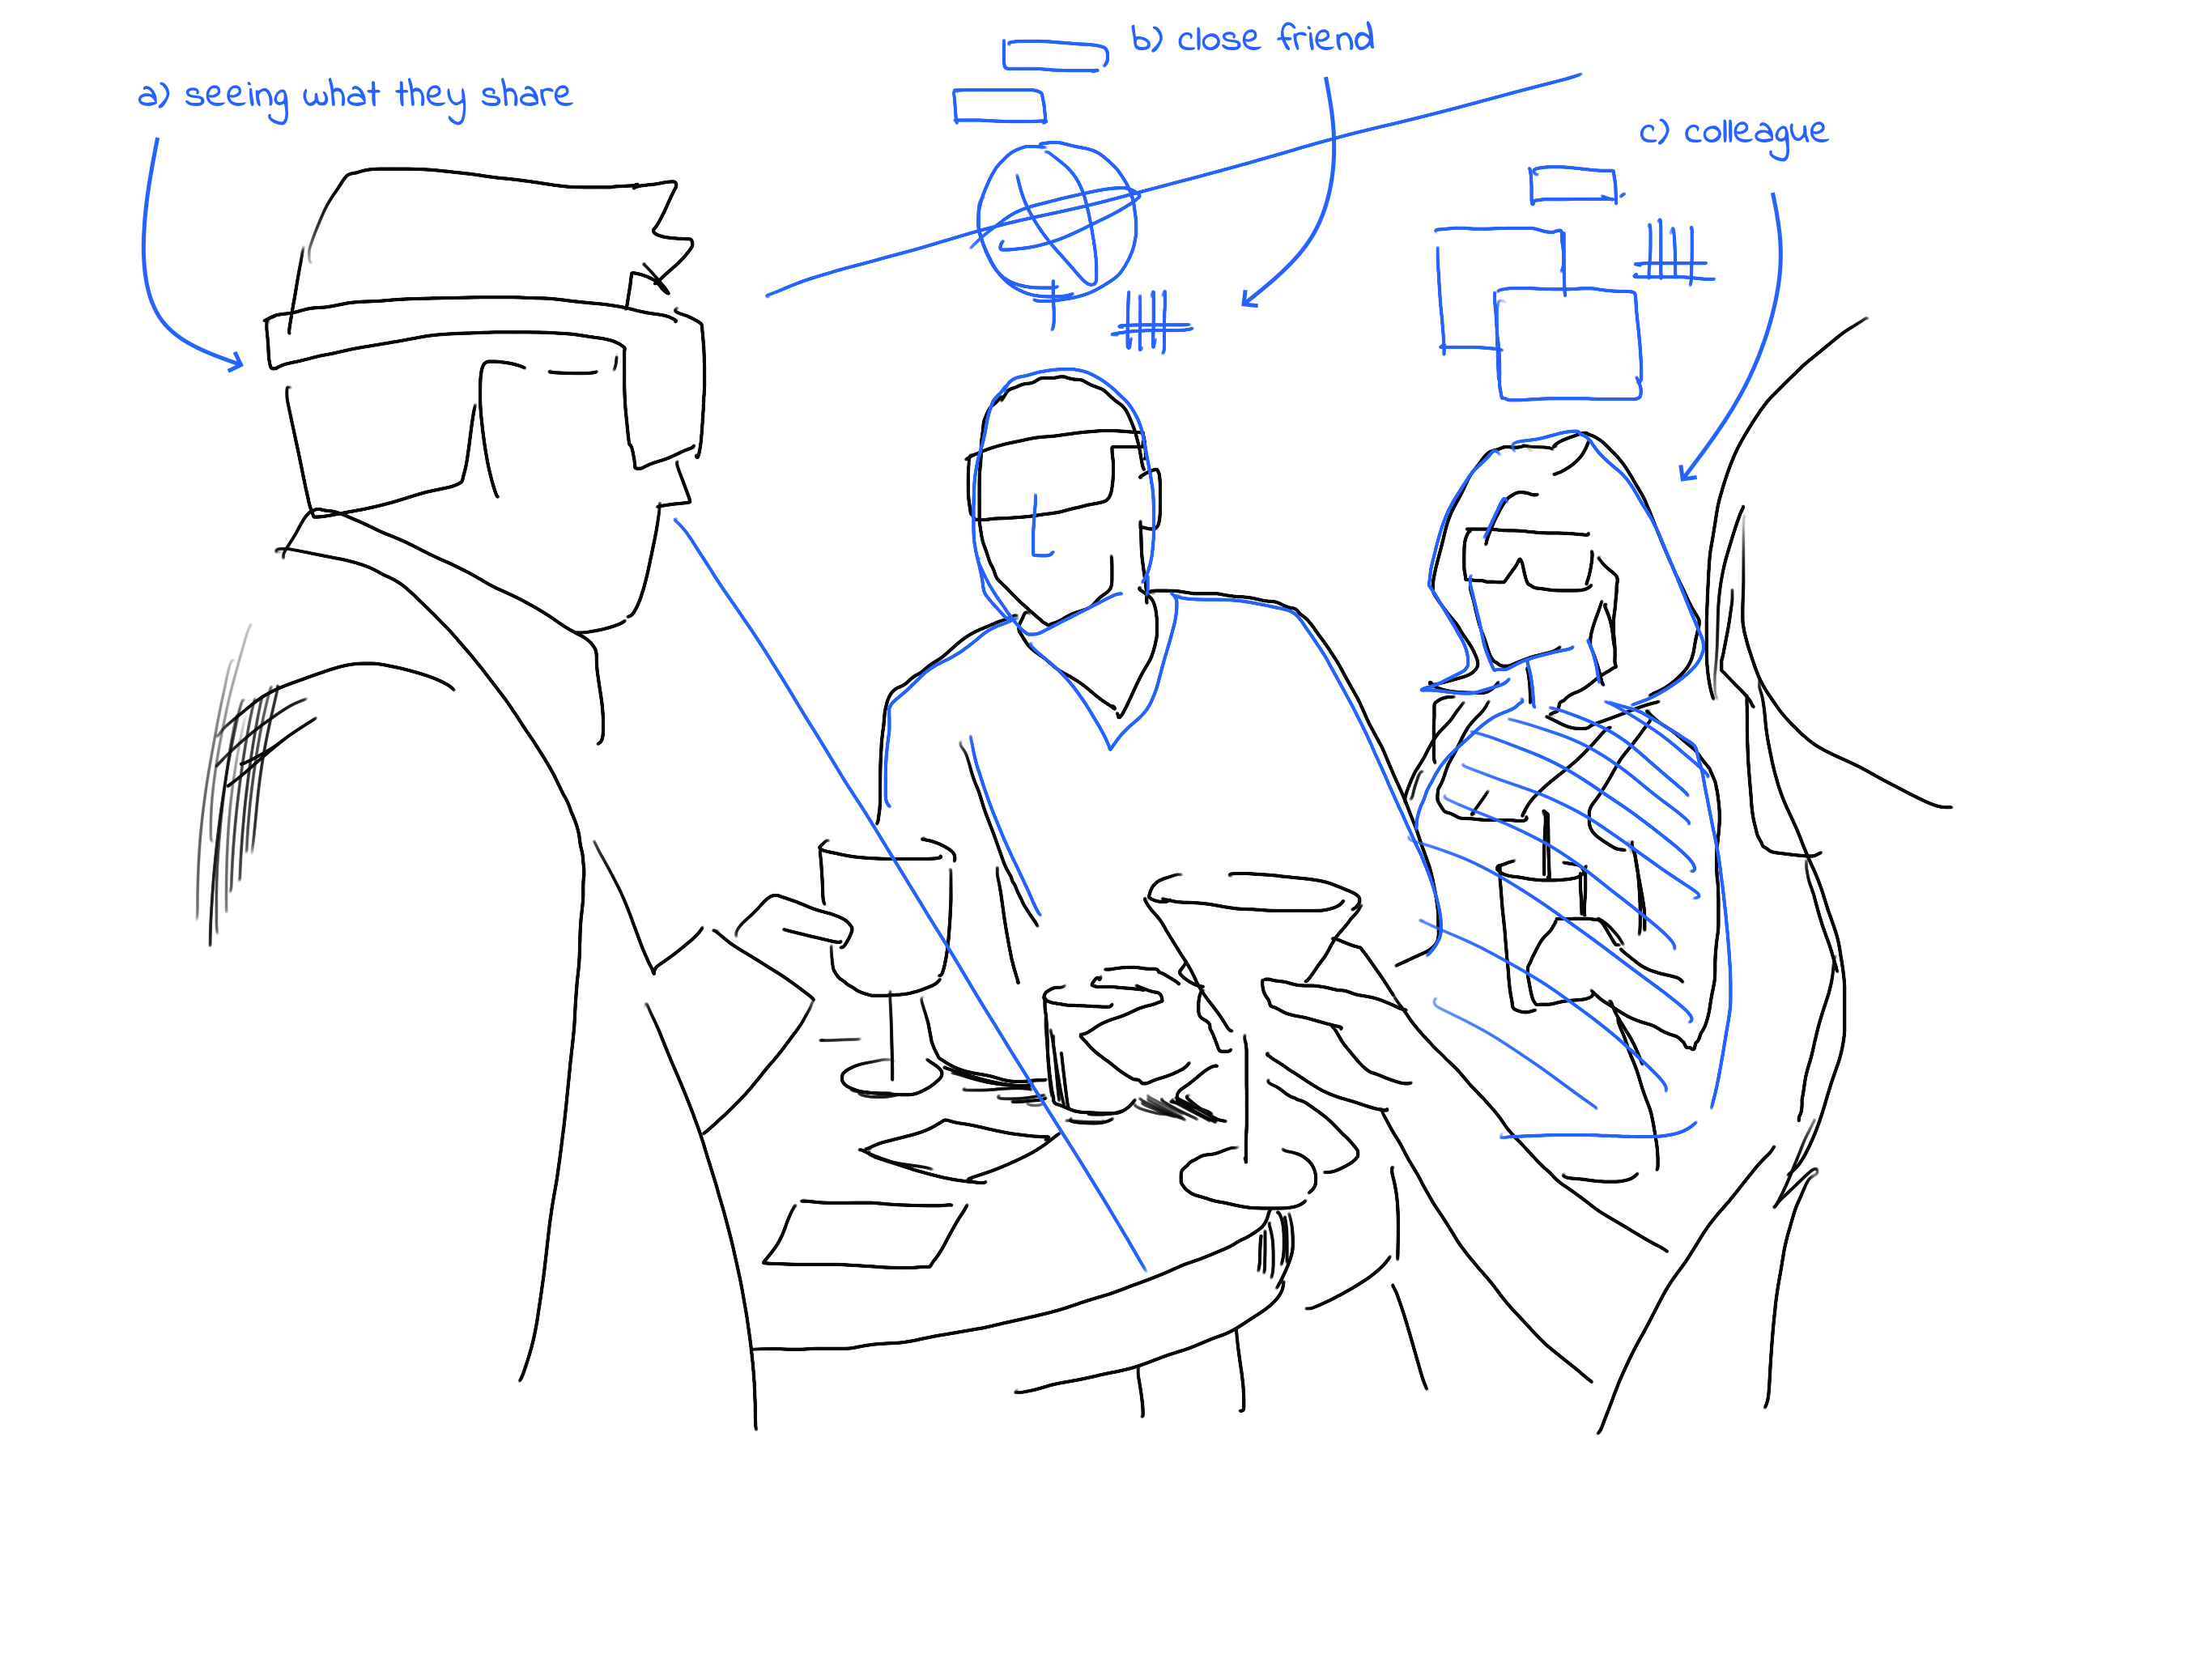
\includegraphics[width=0.8\linewidth]{images/30-continuum/illustrations/3_Bar_Scene.png}
    \caption{Social event scenario. The user meets friends and colleagues face to face at a bar. He sees what they are sharing with him as images/video as AR floating on top of their heads. Based on how socially close with them, he sees more detail (higher fidelity) content from close friends than from strangers or colleagues.  (Illustrated by Kris Tong)}
    \label{fig:illustration:social-event}
\end{figure}

\subsection{Collaborative decoration}

The user is sharing their room (Figure \ref{fig:illustration:remote-bed}) for decoration purposes with 1) a wife, 2) parents, and 3) a friend. The wife will see the full details of the room. The parents see most details, but a few items in the room are blocked/hidden. The friend will see an abstraction of the room with no details. 

\begin{figure}[ht]
    \centering
    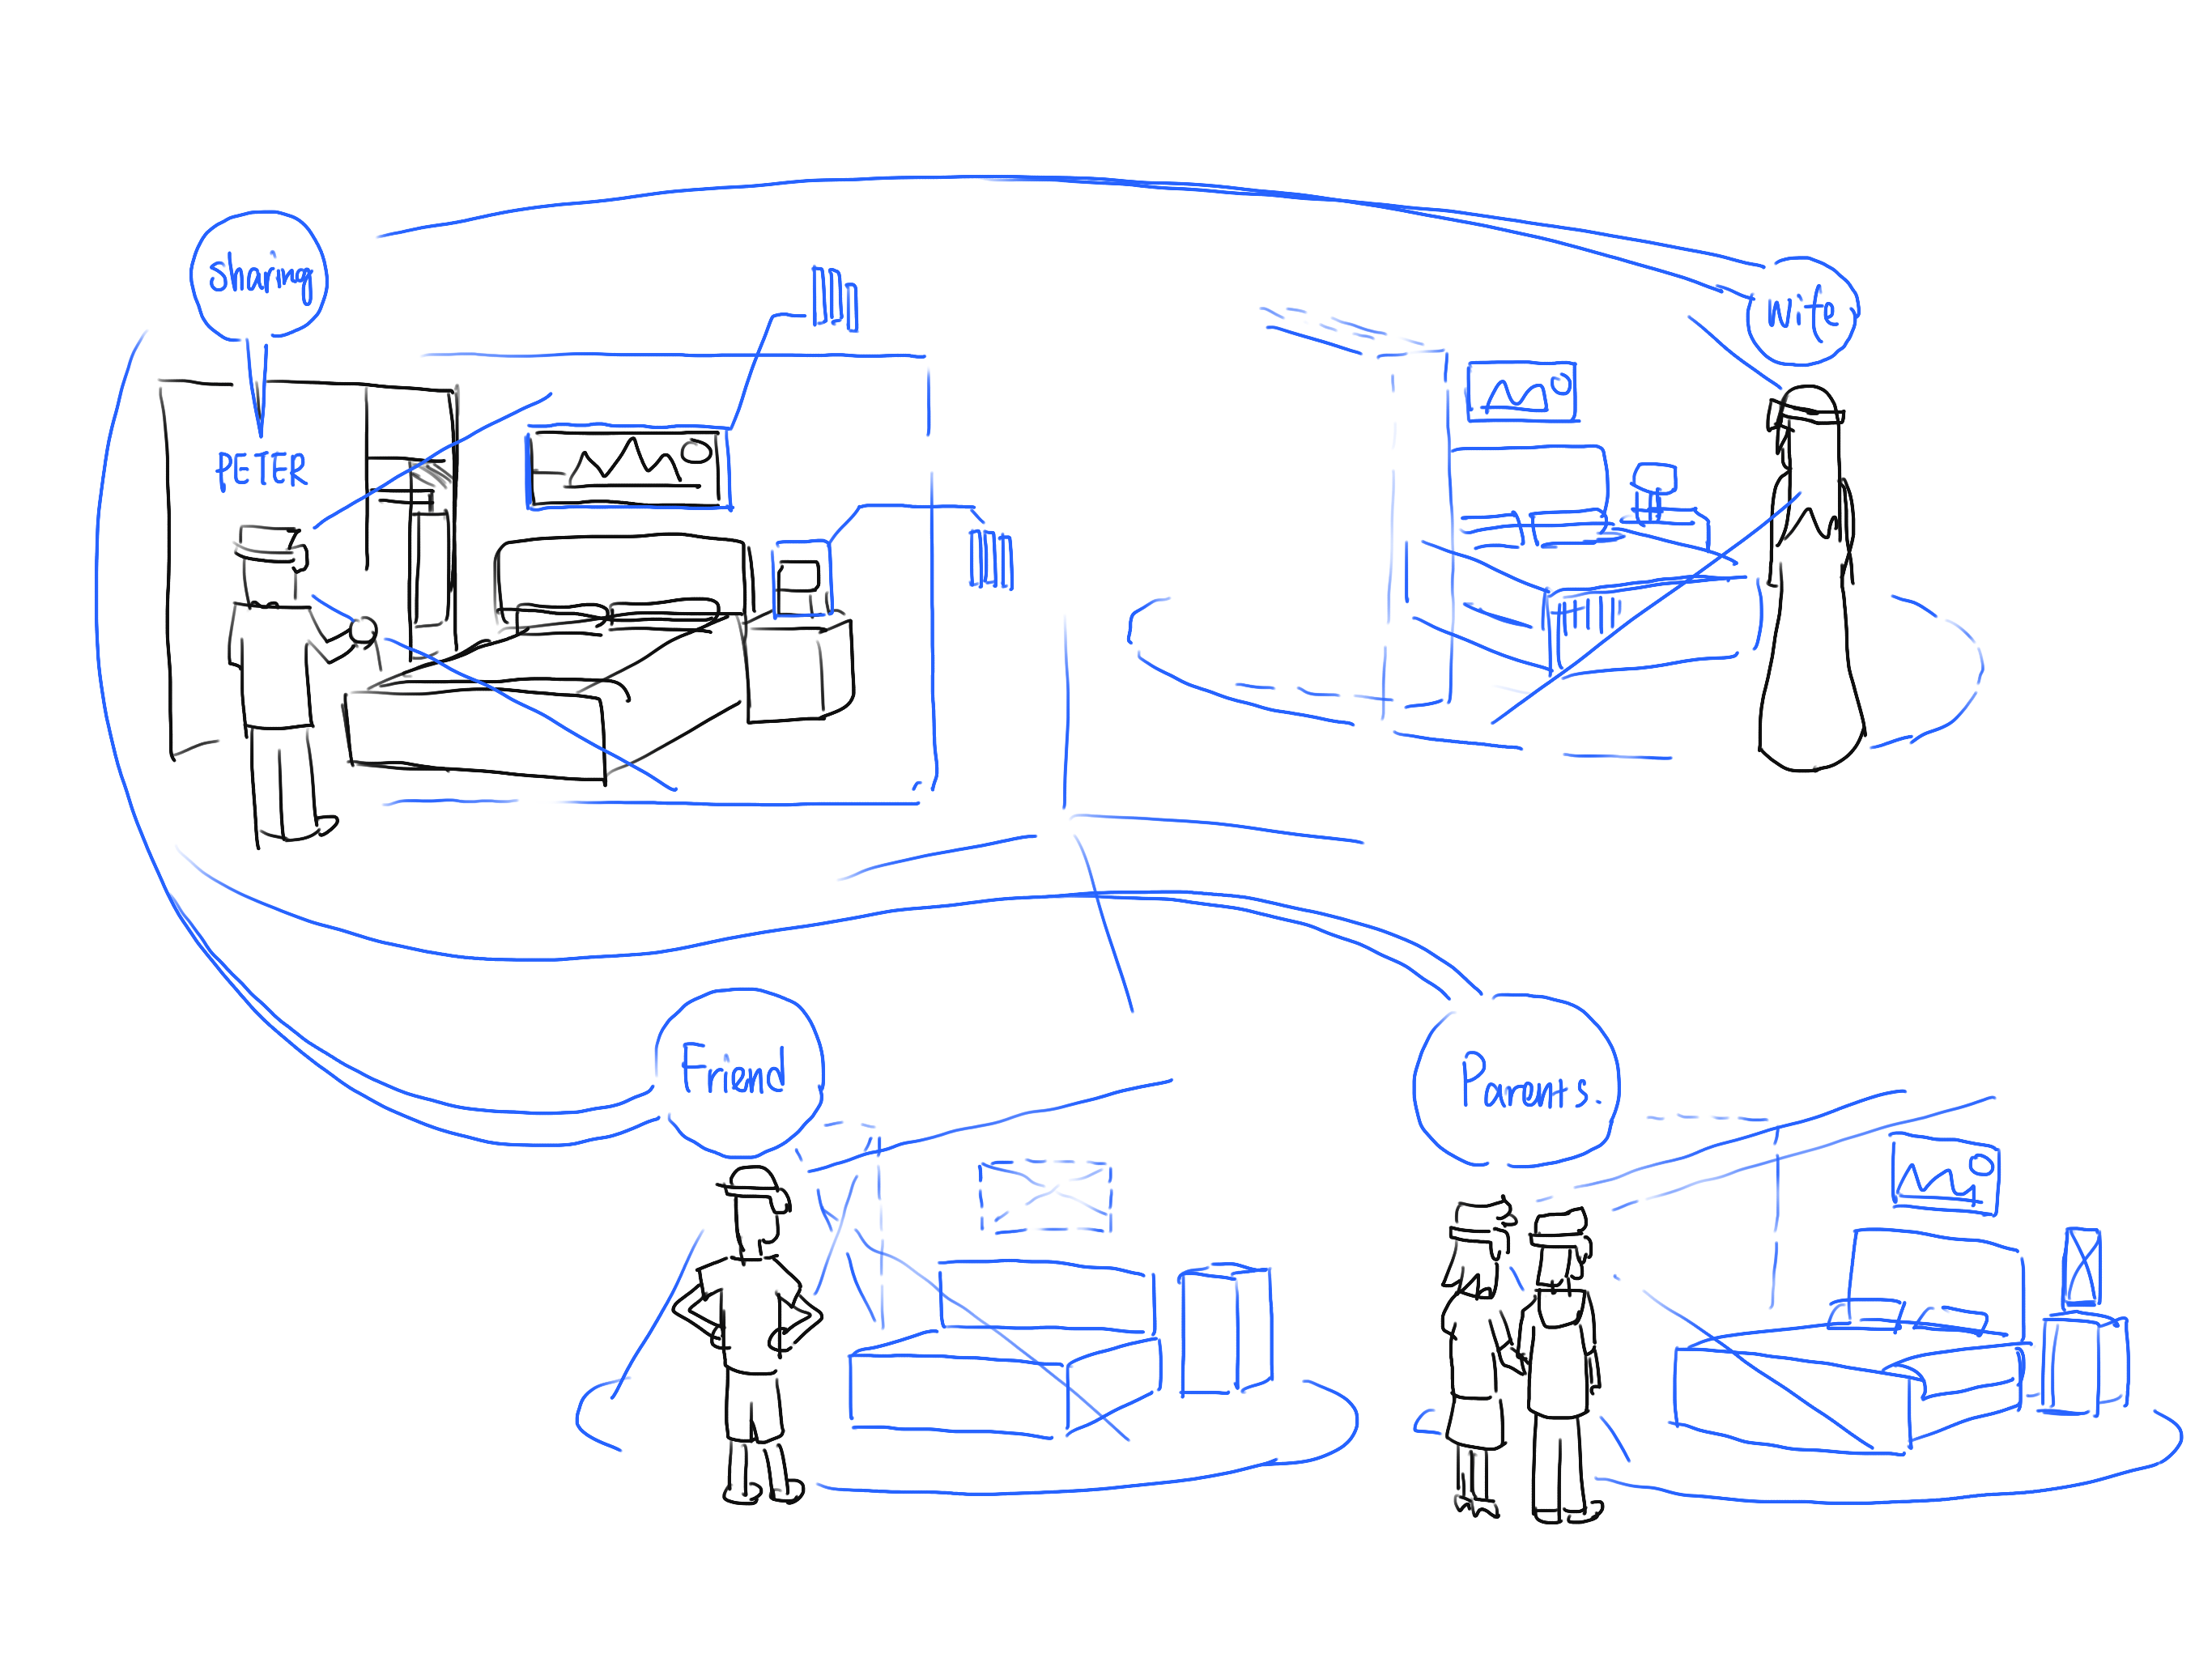
\includegraphics[width=\linewidth]{images/30-continuum/illustrations/1_Remote_Bed.png}
    \caption{Collaborative decoration scenario. The user (top left) shares a 3D scan of his bedroom and invites three people to join in virtually to give suggestions on decorating the room. His wife can see all details about the room and has access to change or add new decorations to the room. His parents can see fewer details about the room than the wife and can give new decoration of furniture items but not change anything in the room. His friend can see a more abstract version of the room and can only give suggestions as text comments.  (Illustrated by Kris Tong)}
    \label{fig:illustration:remote-bed}
\end{figure}

\pagebreak
\section{The Social AR Continuum Dimensions}
% \todo[inline]{ what inspirations? which papers (1/2 page)  initial axes, however realised}
% Tobias: How have you methodologically created the AR continuum: Once you made clear why you need this continuum, you need to also better explain how you have created it. It sounds at the moment a bit like, we need it, and here it is. But how have you created it? Brainstorming alone, with colleagues, any well know HCI approach? A brainstorming meeting with AR professionals could be the answer here but what has driven this brainstorming and what was the overarching idea. Why are certain metrics not in the continuum and could have looked differently? Do you have earlier versions that you can share and explain why they needed more work. I think if you can demonstrate the iterative development that the model underwent, it would support you. In any case you need to explain how you have designed it.

The scenarios of social AR experiences highlighted patterns in terms of how we see others and objects and how to interact with them. Using observation from previous user studies in social AR and inspiration from continuum designs, the concept of a continuum started to crystallise. The Social AR Continuum varies based on the closeness of social connections that we have with others (our relationships), and this thesis identified the following dimensions where social AR applications can fit along a continuum. The dimensions can be grouped in the categories described in Figure \ref{fig:continuum:dimensions}.

\begin{figure}[ht]
    \centering
    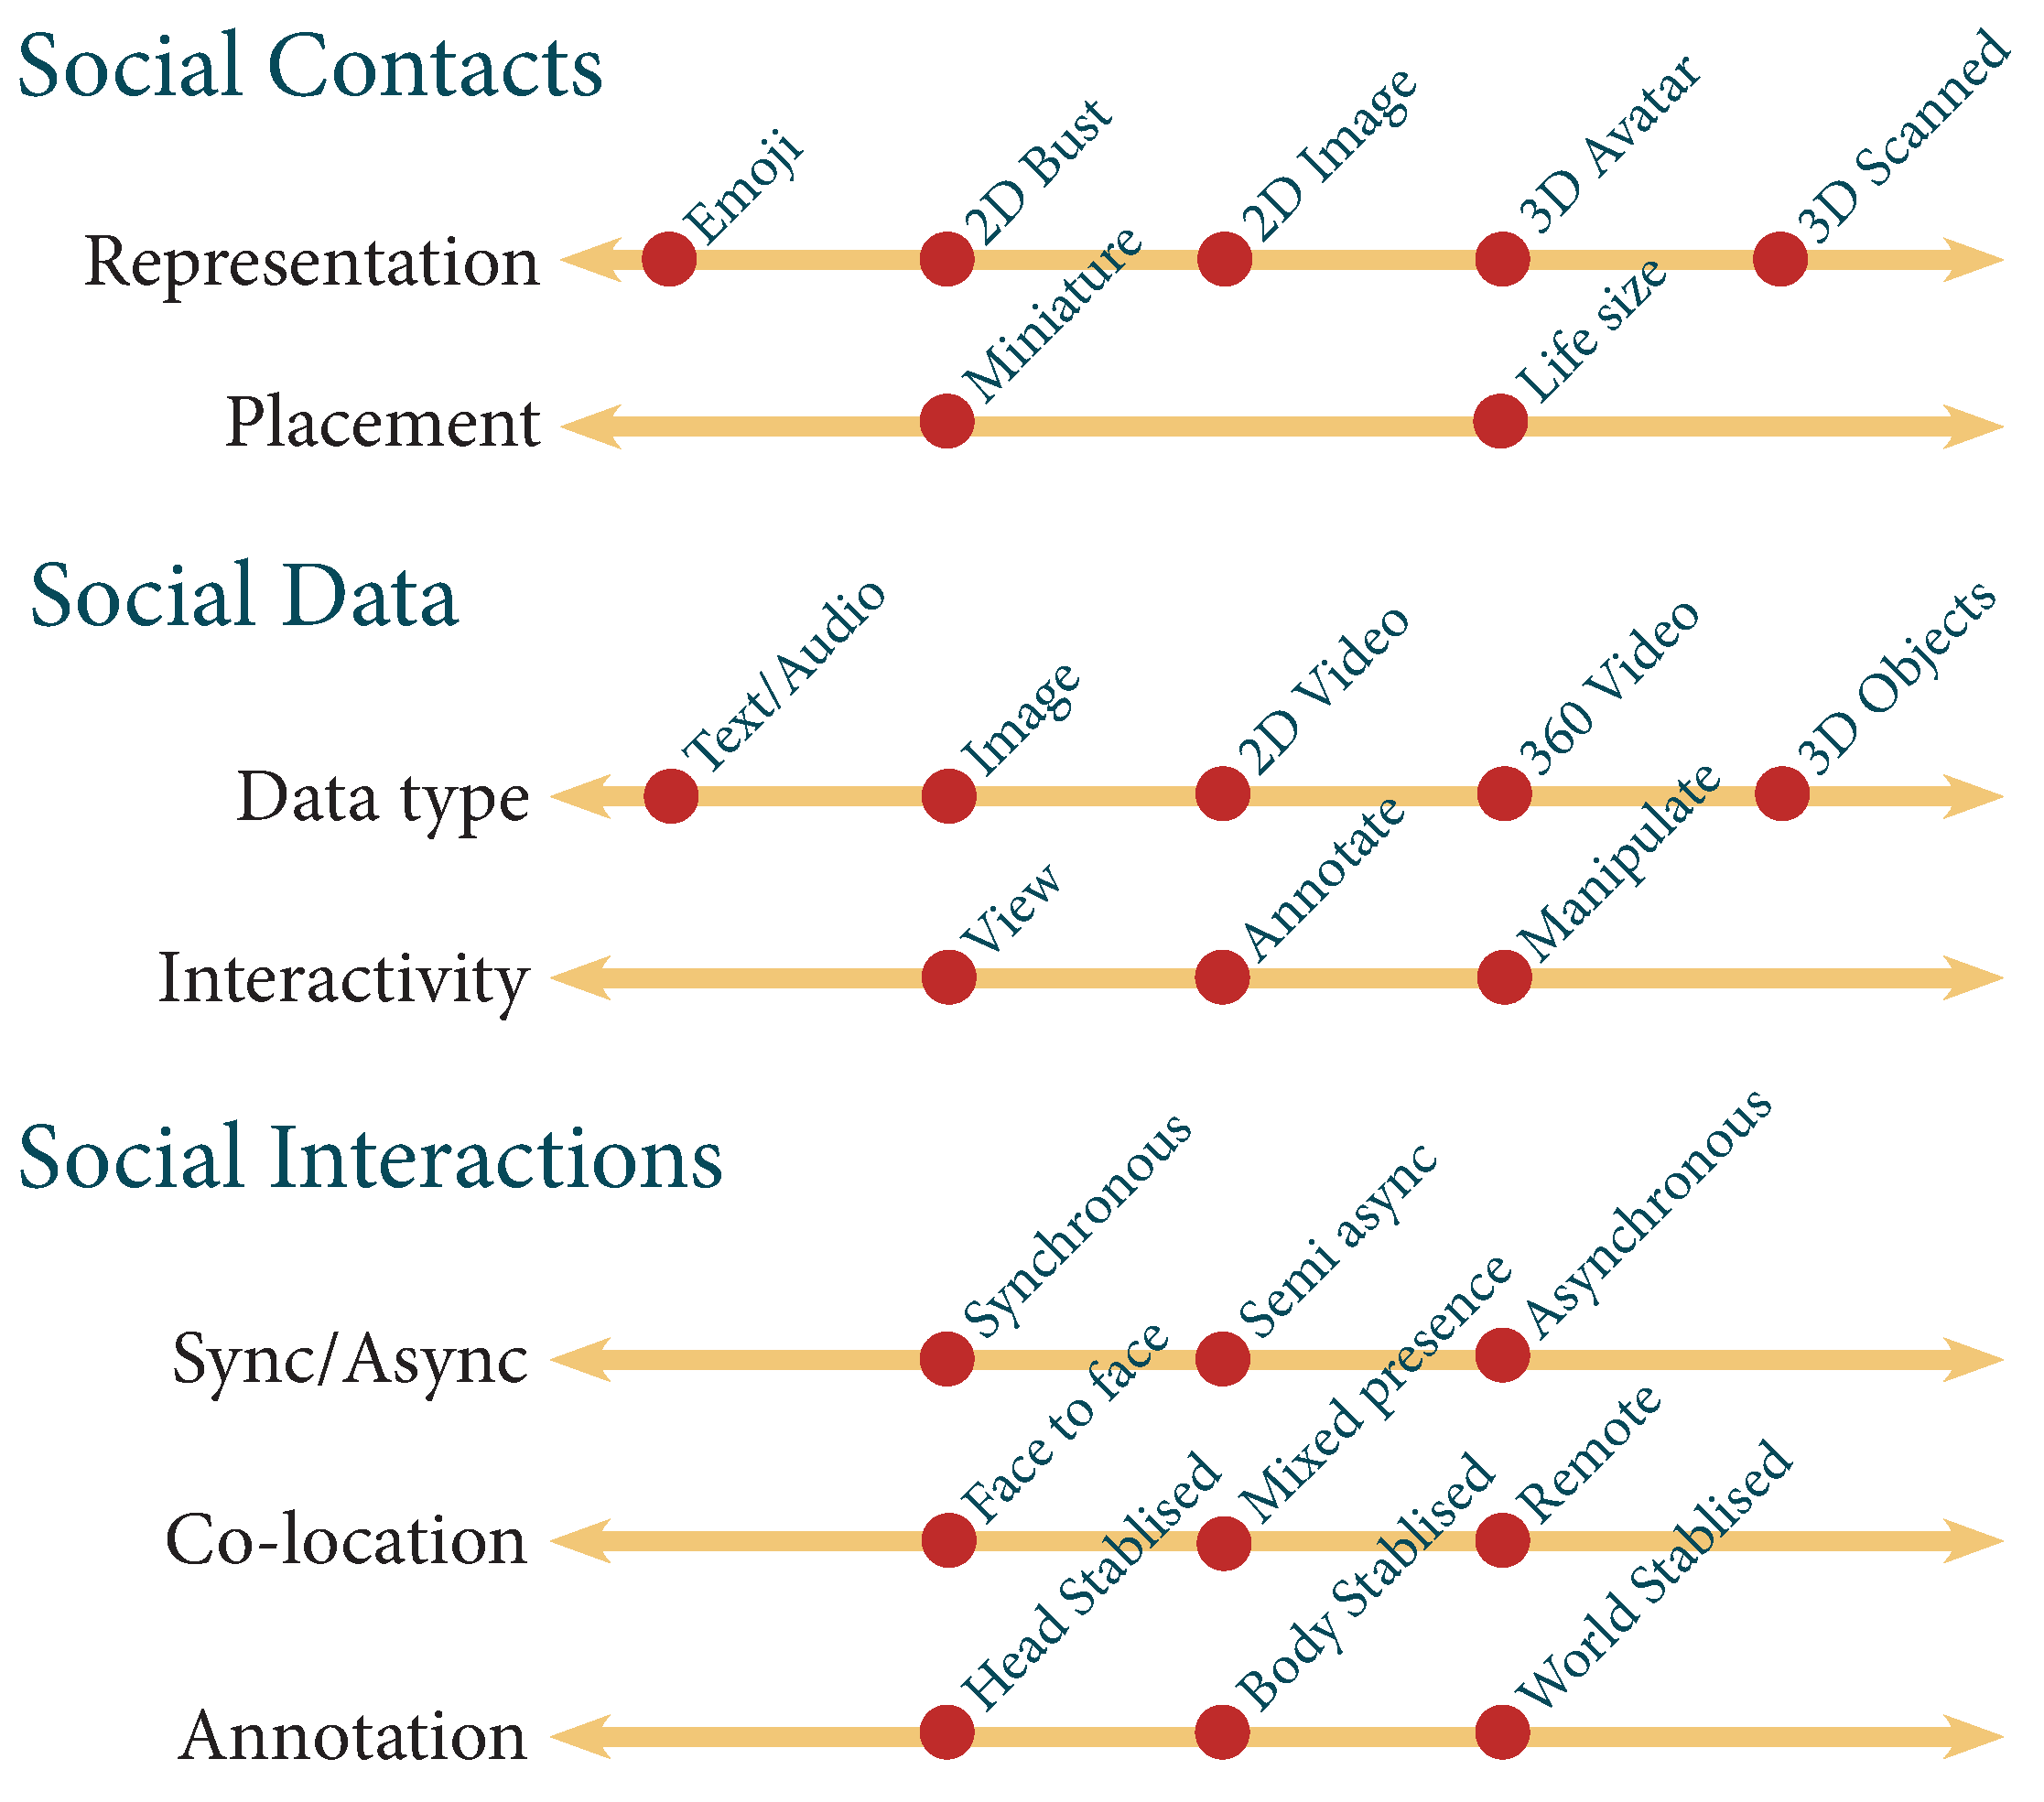
\includegraphics[width=0.8\linewidth]{images/30-continuum/continuum4_1.eps}
    \caption{Dimensions of the Social AR Continuum.}
    \label{fig:continuum:dimensions}
\end{figure}

\subsection{Contact Representation}

Representation of social contacts (Figure \ref{fig:continuum:contact-representations}) can vary on the Social AR Continuum based on the relationship that the user has with the contact, with closer relationships having a higher fidelity representation. For example, \textit{Intimate} contacts could be represented as full 3D animated avatars, \textit{Friends} could be represented as 2D static images, \textit{Acquaintances} could be represented as 2D busts and \textit{Strangers} could be shown as mere emojis. Each contact could choose their representation for each category.

\begin{figure}[ht]
    \centering
    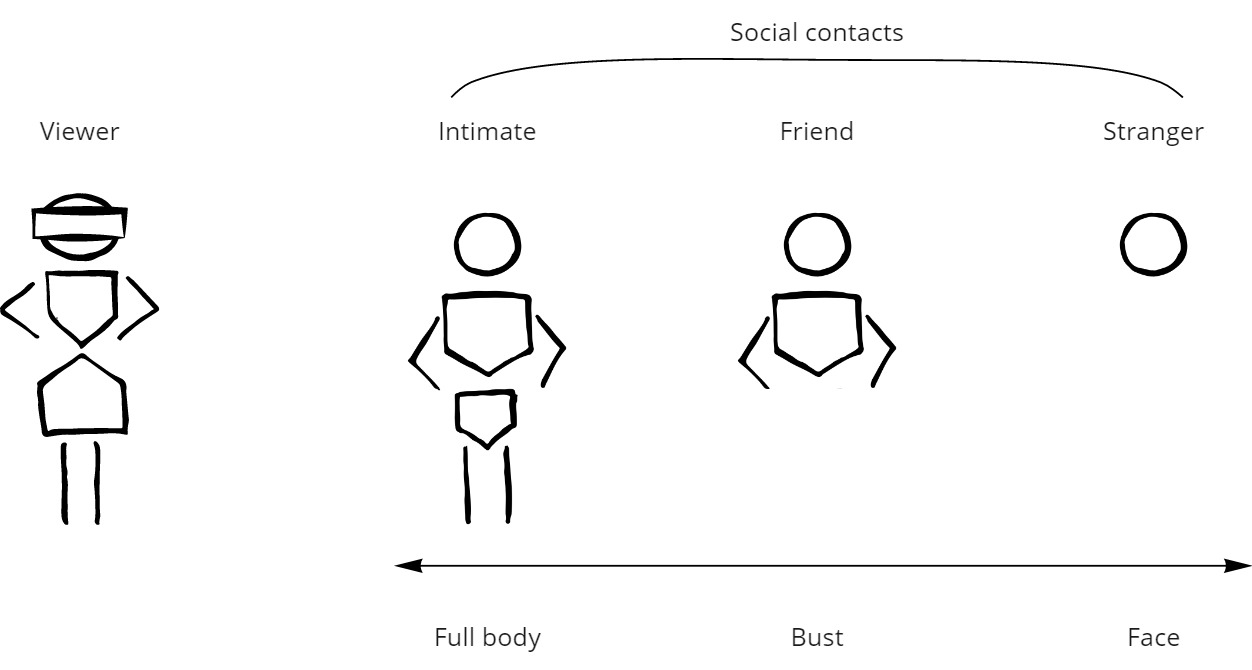
\includegraphics[width=0.8\linewidth]{images/30-continuum/Continuum-representation.jpg}
    \caption{Illustration of contact representations options based on social proximity. An intimate social contact appear in full body to the viewer, while a friend appear in upper half of the body as a 2D image. A stranger appears as an emoticon representing their face.}
    \label{fig:continuum:contact-representations}
\end{figure}

% \textbf{Contact Filter}
% Filtering social contacts to distinguish users from each other could be done using proximity or visual fidelity based on their relationship to the user. Proximity filters contacts by placing them closer or further away. Visual fidelity filters contacts by adding more level of detail to the contact for closer relationships and less detail for further away contacts. 

\subsection{Contact Placement}

Placing social contacts (Figure \ref{fig:continuum:contact-placement}) can be done by displaying \textit{Intimates} as life-sized avatars on the ground around the user, and others as miniatures on a nearby surface. 

\begin{figure}[ht]
    \centering
    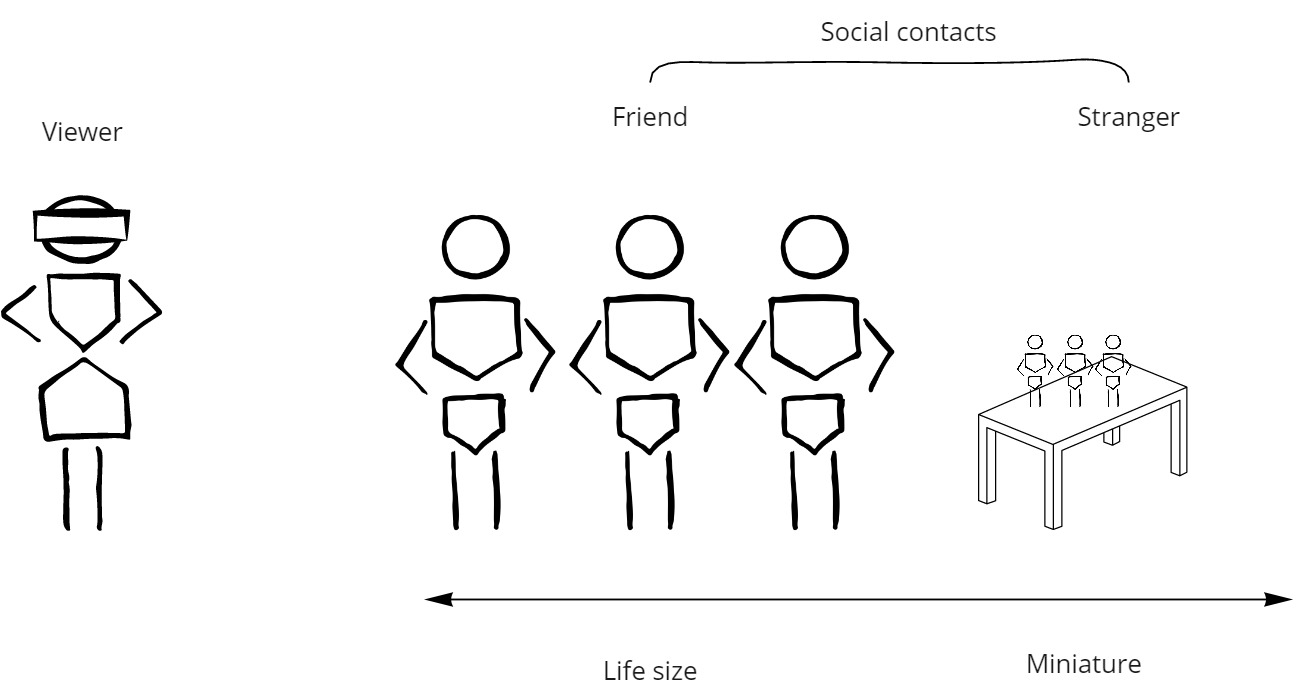
\includegraphics[width=0.8\linewidth]{images/30-continuum/Continuum-placement.jpg}
    \caption{Illustration of Contact placement options based on social proximity. Close friends can be displayed as life-size avatars, while other can be displayed as a miniature figures.}
    \label{fig:continuum:contact-placement}
\end{figure}

% \subsection{Contact transparency}
% \todo[inline]{Add illustration}


% The transparency of social contacts can be used based on social proximity. Closer social contacts appear more opaque while further away ones appear more transparent.

\subsection{Data Type}

The type of data (Figure \ref{fig:continuum:data-type}) shared between social contacts in AR could be categorised as 1D (e.g., text or audio), 2D (e.g., images, panorama or video), or 3D (e.g., 3D model or scanned-room environment). Based on the relationship between the user and their social contacts, the type of data available could be filtered. For instance, 3D data could be shared with \textit{Intimate} relationships, while \textit{Acquaintances} could see only 2D data.  

\begin{figure}[ht]
    \centering
    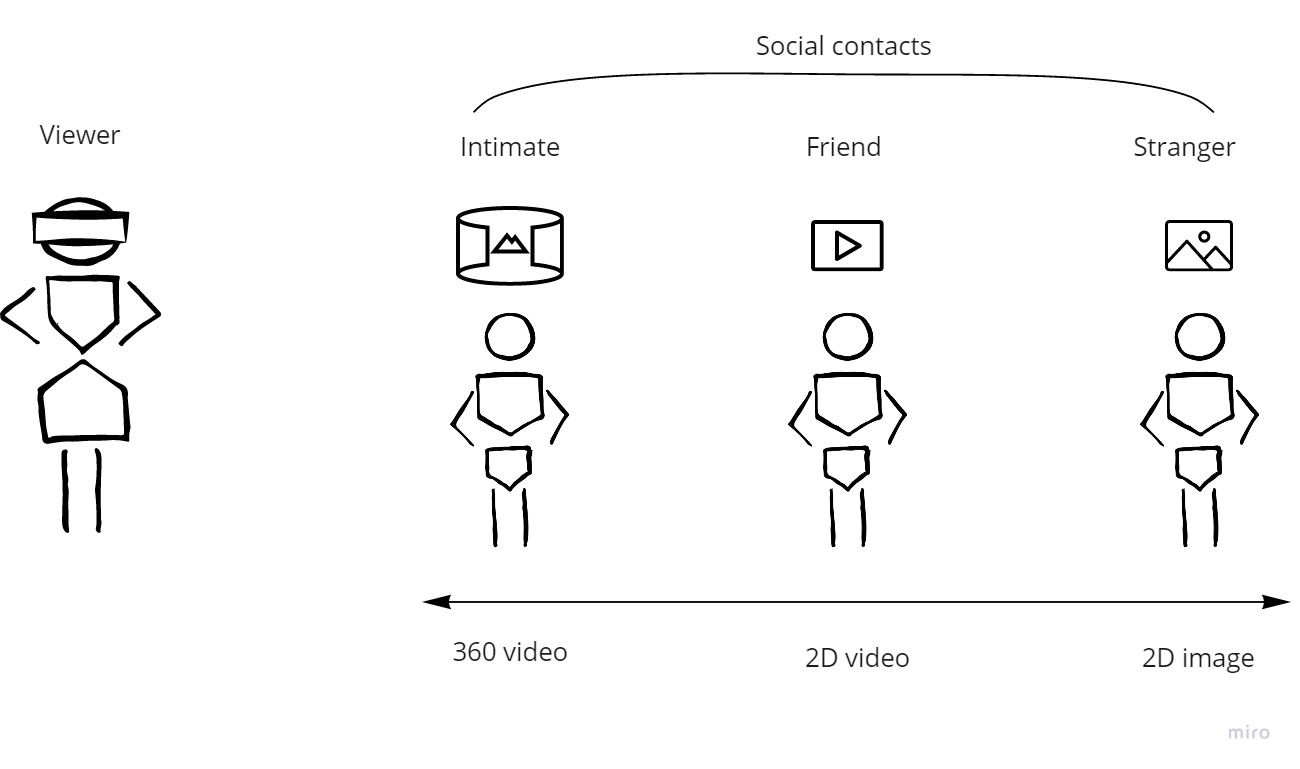
\includegraphics[width=0.8\linewidth]{images/30-continuum/Continuum-Data-type.jpg}
    \caption{Illustration of data type options. Close social contacts can see higher fidelity of shared data than the socially further away ones}
    \label{fig:continuum:data-type}
\end{figure}

\subsection{Data Interactivity}

In terms of user interactions (Figure \ref{fig:continuum:data-interaction}) with shared data, the Social AR Continuum here ranges from viewing the contents, annotating or adding comments on the content, through to manipulating the content. Levels of manipulation include changing the position, rotation or scale of the shared content, or even modifying the content itself.

\begin{figure}[ht]
    \centering
    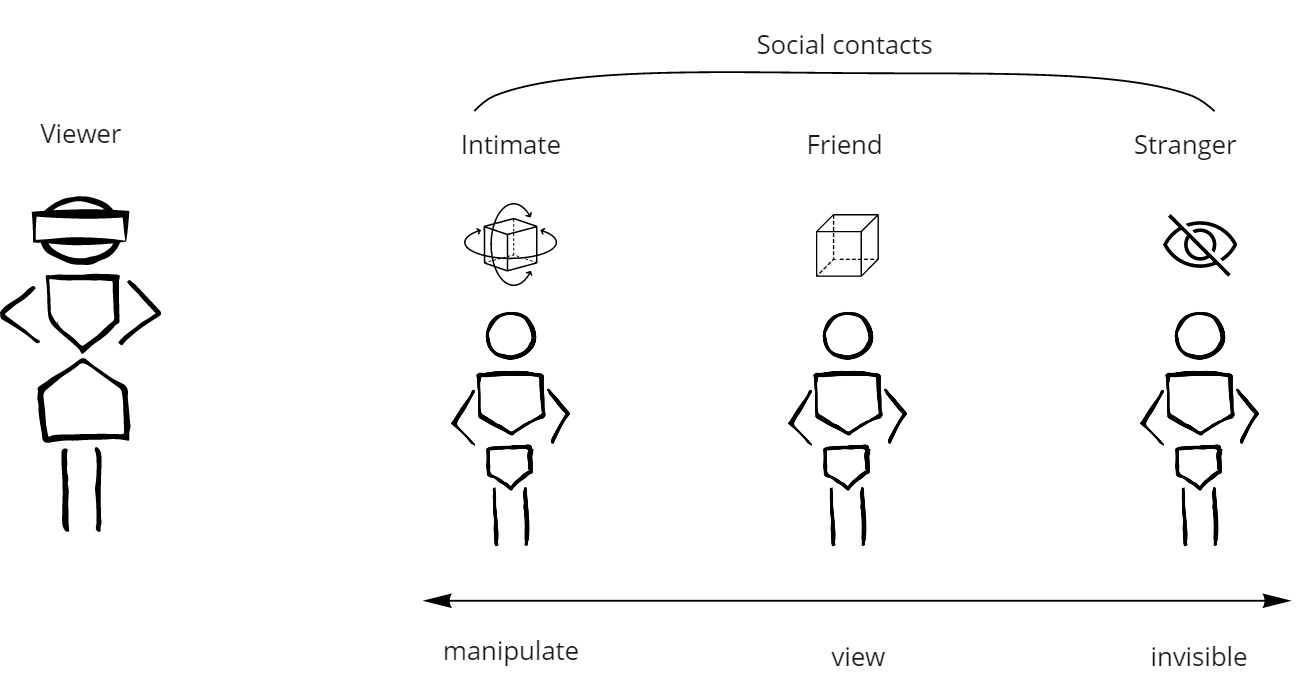
\includegraphics[width=0.8\linewidth]{images/30-continuum/Continuum-interaction.jpg}
    \caption{Illustration of data interactivity options. Closer social contacts can interact with the shared data in higher fidelity (add/edit/remote) than the further away ones (view only)}
    \label{fig:continuum:data-interaction}
\end{figure}

% \subsection{Data Privacy}
% \todo[inline]{Add this to the dimensions figure}

% Based on the relationship with other users, shared data can be made private to the user, shared with specific groups of people (e.g., friends, acquaintances), or shared with everyone. This will allow users to choose the privacy levels of the shared data based on their social relationship with others. 

\subsection{Synchronous/Asynchronous Data}

The synchronicity of the shared data (Figure \ref{fig:continuum:data-connection}) can be represented based on social proximity. The data shared with contacts could be shared in a synchronous way, where both sharing and interaction happen at the same time. In contrast, data could also be shared asynchronously \cite{Smith2016}, i.e., interaction happens at a different time. 

\begin{figure}[ht]
    \centering
    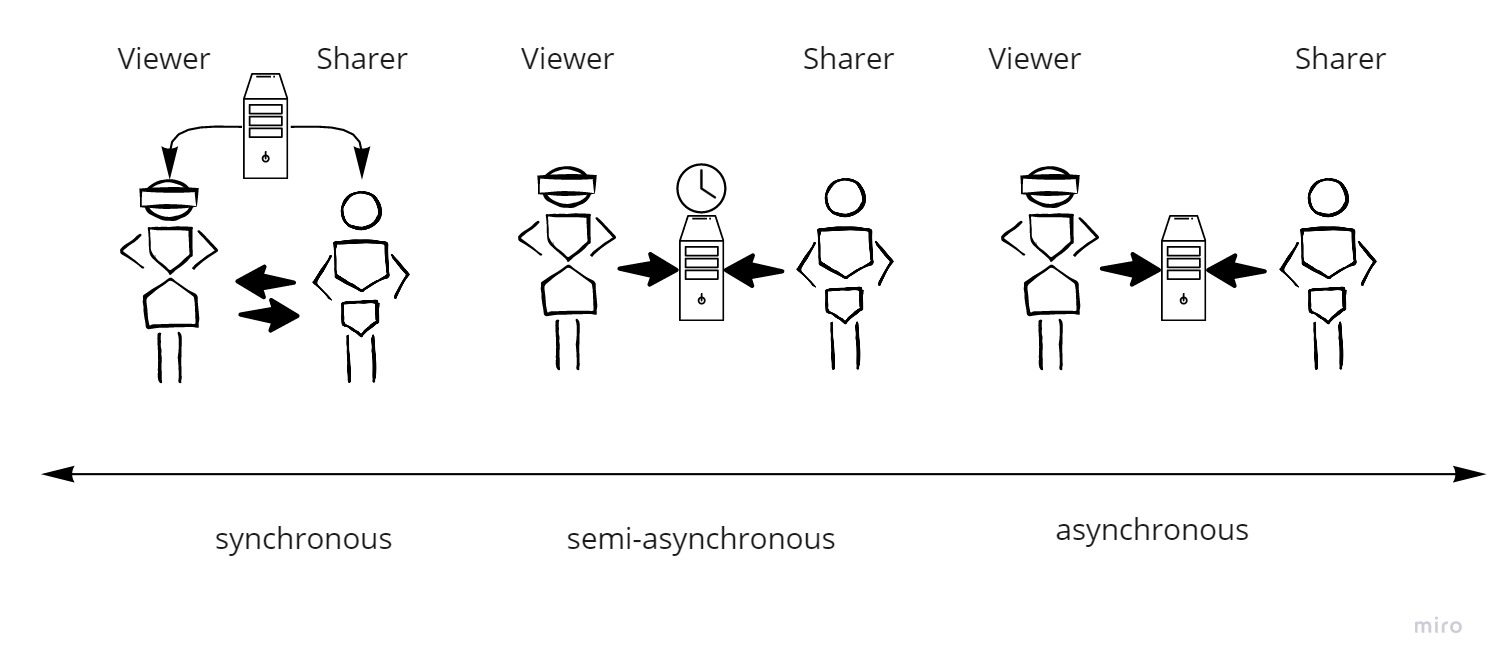
\includegraphics[width=0.8\linewidth]{images/30-continuum/continuum-connection.jpg}
    \caption{Illustration of data connection options.}
    \label{fig:continuum:data-connection}
\end{figure}

\subsection{Co-location}

% \todo[inline]{Gun Lee: This sounds more generic concept in collaboration, rather than having social aspects. I.e. would colocation controlled/adjusted depending on social proximity as you do with other dimensions? Or would this be merely a description of collaborative scenarios?}

The co-location of the social contacts and their interactions (Figure \ref{fig:continuum:data-colocation}) can be represented based on social proximity. Options for representing social people or data can be in: 
1) remote (i.e., in a different place than the user), 
2) face-to-face (i.e., physically in the same location as the user), or 
3) semi face-to-face (i.e., where the social contact/data is physically in the same location, but virtually hidden or removed). When social contacts are remote, they are represented as virtual avatars based on their relationship with the user. When social contacts are face to face, then AR information is displayed attached to their body (i.e., when social contact moves, the information moves with them). 
An example of a semi face-to-face interaction was described in a Black Mirror\footnote{http://www.imdb.com/title/tt2085059/} episode "White Christmas" where a person could 'block' another co-located person by blurring them out in their AR view of the real world.

\begin{figure}[ht]
    \centering
    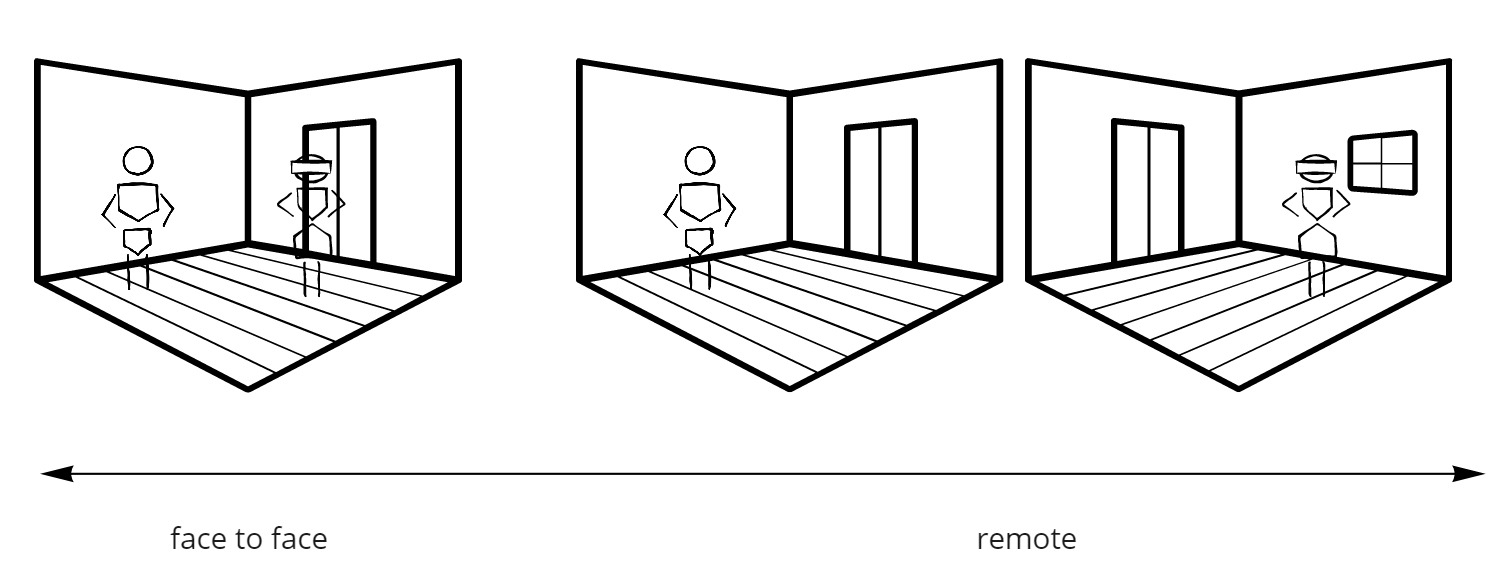
\includegraphics[width=0.8\linewidth]{images/30-continuum/continuum-colocation.jpg}
    \caption{Illustration of data co-location options.}
    \label{fig:continuum:data-colocation}
\end{figure}


\subsection{Annotation}
% \todo[inline]{Add illustration}

Placing AR annotations (Figure \ref{fig:continuum:data-annotation}) or information attached to an AR object can be described as head-stabilised, body-stabilised or world-stabilised \cite{Billinghurst1998}. When adding text to describe an object or a place, the text can be placed as a list (lower fidelity) on the side of the screen or can be placed on the related object as an AR annotation (higher fidelity) that "sticks" to the scene and disappears if the user looks away. This dimension can be used with social contacts, and if the contact is a close friend, they would see the annotation in higher fidelity, while a stranger would see the text annotation in lower fidelity. 

% \todo[inline]{Rob: Seems odd. Do you mean they might see that there is an annotation , but can not read it?}

\begin{figure}[ht]
    \centering
    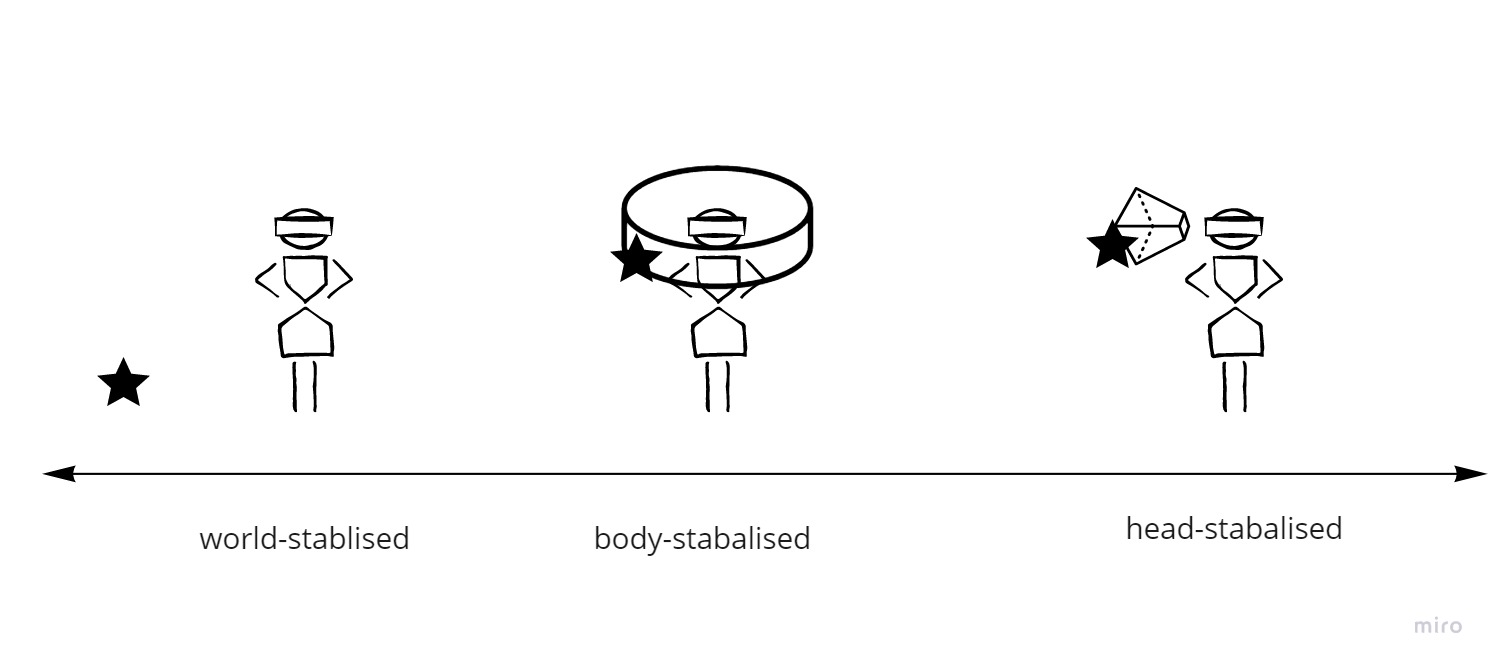
\includegraphics[width=0.8\linewidth]{images/30-continuum/continuum-annotation.jpg}
    \caption{Illustration of data annotation options.}
    \label{fig:continuum:data-annotation}
\end{figure}

% gogo: Another way to think about list vs. callouts is view-fixed (list) versus world-fixed (callouts). Feiner (I think it was him) defined a set of locations/things that text/windows could be attached to


% \subsection{Collaboration}
% When collaborating with social contacts, the user could use a pointer (e.g. arrow, indicator) to direct the conversation to a particular place or use a drawing tool (e.g. a pencil) to highlight the area of the conversation. The availability of these options could depend on the social proximity between social contacts. If closer to each other, higher fidelity tools are available, and if strangers, then the collaboration is limited to lower fidelity tools.

% \subsection{Awareness}

% It is possible during a session of sharing social experiences, that social contacts are looking in different directions. Awareness tools help users to know where the other user is looking. This can be achieved by showing a rectangle or a circle pointing to where the user is looking, or by using a context compass view which provides higher fidelity for closer connections.

% Gun: add a bit more details on how controlling each dimension based on social proximity would benefit

\section{Summary}

This work introduced the concept of the Social AR Continuum and identified several dimensions where a social AR application could be implemented.
In the next chapters, 
this thesis explores three categories on the Social AR Continuum through system prototypes and user studies.
explores the three categories on the Social AR Continuum by describing system prototypes and user studies. 

% Gun: close this chapter by giving an overview of the next few chapters.
%checked by Mark - May 9th 2019
\chapter{Social Contacts in AR}
\label{ch:contacts} 

The previous chapter presented the concept of the Social AR Continuum, together with examples for its relevance. This work identifies the representation of social contacts as one of the main dimensions within our social AR continuum. Here, this section distinguishes in particular how to present social contacts (e.g. visual fidelity) and where to present them (spatial mapping such as proximity). This chapter then expands by focusing on this dimension and explore different visualisation types along this dimension. 

This chapter focuses on how to represent social contacts through a wearable AR device. The aim is to answer the research question \ref{rq:people}: \textit{What dimensions work best for visualising and interacting with social contacts through wearable AR displays?}. This chapter aims to answer this question by exploring two dimensions of the Social AR Continuum: 1) representing social contacts and 2) placement of social contacts (Figure \ref{fig:contacts:contacts-continuum}. The representation of social contact varies based on their relationship with the user. 
The first section (\ref{sec:contacts:visualising}) looks into options of visualising social contacts as avatars with multiple levels of detail. The second section (\ref{sec:contacts:placing}) looks into options for placement of social contacts. 

\begin{figure}[h]
  \centering
  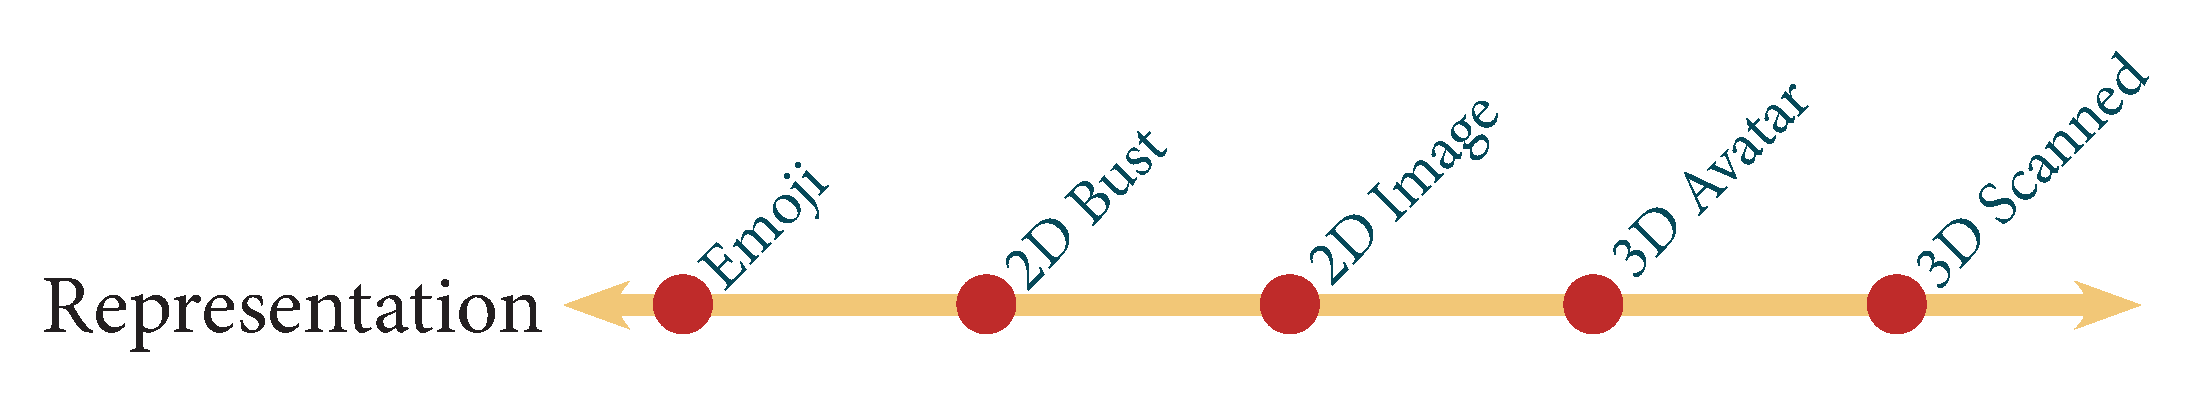
\includegraphics[width=\columnwidth]{images/continuum/continuum4.2-01.eps}
  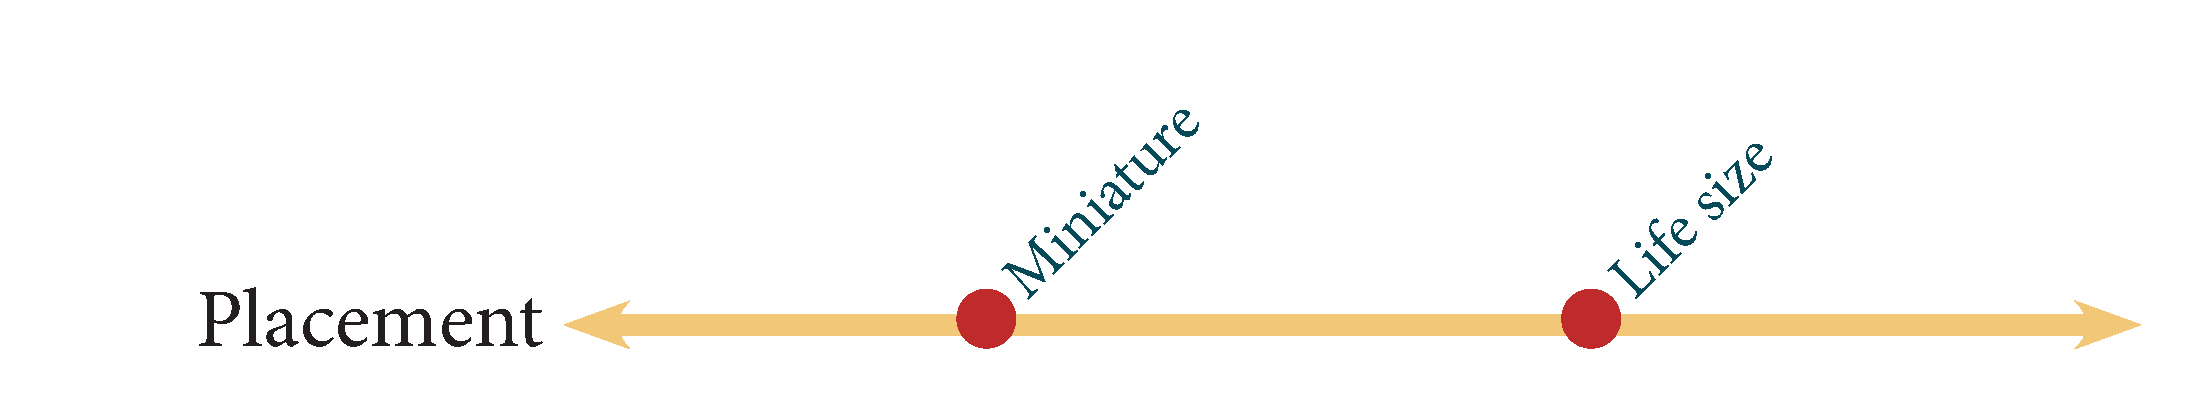
\includegraphics[width=\columnwidth]{images/continuum/continuum4.2-02.eps}
  \caption{Social contacts continuum}
  \label{fig:contacts:contacts-continuum}
\end{figure}

% Gun Lee: Give a recap of the "People" dimensions you defined in Chapter 3 to give context on why and how the following sections link back to these concepts.

%checked by Mark May 9th 2019
\section{Proximity and Visual Fidelity}
\label{sec:contacts:visualising}

As part of the Social AR Continuum, representing social contacts of self and others is one of the main dimensions. This section explores representing social contacts in the form of avatars in AR. 

One of the issues with representing contacts from social networks in AR is how to differentiate between the contacts. This section explores how visual and spatial cues based on social relationships can be used to represent contacts in social AR applications, making it easier to distinguish between them \cite{Nassani2017b}. This section explores how to visualise social relationships in mobile AR environments using proximity and visual fidelity filters. A focus group was organised to explore different options for representing social contacts in a mobile AR application. Also, a user study was conducted to test a head-worn AR prototype using proximity and visual fidelity filters. 

Visualising of social contacts traditionally has been represented as a list of names and a profile photo, which can be found in popular social networking mobile and web apps such as Facebook\footnote{https://www.facebook.com/}, Whatsapp\footnote{https://www.whatsapp.com/}, LinkedIn\footnote{https://www.whatsapp.com/} and others. In Google\texttt{+} \footnote{https://en.wikipedia.org/wiki/Google\%2B}, social contacts are represented as a graph of circles interconnected based on common interest and how people know each other. In Snapchat\footnote{https://www.snapchat.com/}, social contacts are also represented as a list in addition to a map feature where it shows friends as avatars overlaid on a map based on their geographical location. The avatars in Snapchat are created using Bitmoji\footnote{https://www.bitmoji.com/}, which allows the user to customise the appearance of their avatar that can be used to express predefined gestures representing emotions and interactions. Snapchat also uses these Bitmoji in sharing an AR scene where the avatar is overlaid on the camera view of a handheld device. 

The focus of this research is on how to represent a social network with hundreds of contacts in a wearable AR interface. If there are dozens of virtual tags in an AR view representing people, how can they be distinguished between each other? How will this scale to hundreds or thousands of people? The importance of this research is that it will allow users to view and interact with a large number of social network followers at different levels of privacy and social engagement.

Allowing users to view and interact with a large number of social contacts requires filtering and categorising information. One way to filter/categorise contacts could be to arrange them along a social continuum, depending on how close (in terms of social proximity) they are to the user. For example, grouping people into Intimate Family, Friends, Colleagues, and Strangers (see Table \ref{tbl:visual-fidelity-proximity}), or more categories. Contacts from these categories could then be shown as virtual avatars with different levels of visual fidelity and visual proximity, enabling the user to identify people in their social network quickly.

\begin{table}[h]
    \centering
    \caption{Using Visual Fidelity and Visual Proximity to Categorise Friends}
    \label{tbl:visual-fidelity-proximity}
    \begin{tabular}{|l|l|l|}
        \hline
        \textbf{Category} & \textbf{Visual Fidelity}    & \textbf{Visual Proximity}       \\ \hline
        Intimate          & 3D avatar                     & \textless1m, same space  \\ \hline
        Close friend      & 2D avatar                   & 1-5m, close              \\ \hline
        Acquaintance      & Bust image                    & 5-20m, nearby            \\ \hline
        Stranger          & Emoji                        & \textgreater20m, distant \\ \hline
    \end{tabular}
\end{table}


In terms of Visual Fidelity, the representations of people in each of these categories could be increasingly more realistic as the categories changed from Stranger to Intimate Family (see Figure \ref{fig:contacts:visual-fidelity-continuum}). For example, a user may see their spouse as a realistic 3D virtual human superimposed over the real world, but a distant acquaintance would be a simple 2D icon.

\begin{figure}[h]
    \centering
    \includegraphics[width=0.8\linewidth]{images/41-visualising-mgia17/writing-images-07.eps}
    \caption{Changing Visual Fidelity across the social continuum}
    \label{fig:contacts:visual-fidelity-continuum}
\end{figure}

In terms of proximity, previous studies have shown that the distance between people in social settings varies according to their level of intimacy \cite{Anslow2016}. This can be used to place the virtual representations of people in the real world around the user. The people that are Intimate family and Friends could be shown as visually closer to the user, while people who are Strangers would be shown further away (see Figure \ref{fig:contacts:proximic-circles}). This can be implemented as a body-centric virtual information space that travels with the user when they move.

The combination of using Visual Fidelity and Visual Proximity to categorise people from a user's social network could make it significantly easier for the viewer to pay attention to the people that they want to. For example, close Friends are represented as life-like virtual avatars near to the user, and so are easily distinguished from Strangers that are emoji icons further away.

\begin{figure}[h]
  \centering
  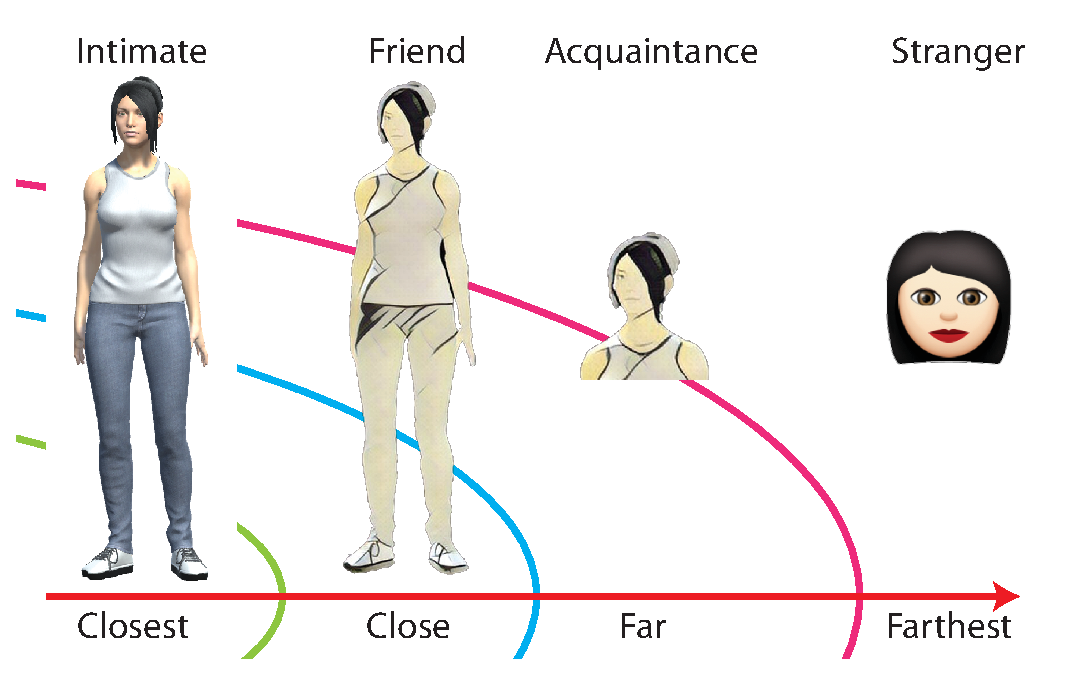
\includegraphics[width=0.8\linewidth]{images/41-visualising-mgia17/writing-images-11.eps}
  \caption{Visual Proxemic \& Visual Fidelity Filtering of Avatars}
    \label{fig:contacts:proximic-circles}
\end{figure}

% Other cues could be explored as well, such as placing people closer to the centre of the visual field who are more critical/active, using colour to distinguish which users are currently available, or providing spatial audio cues to guide a person's attention.


\subsection{Implementation}

Using the Social AR Continuum metaphor from the previous section, this work developed a prototype on the Microsoft HoloLens to represent a user's social contacts in an AR environment. The prototype was built using Unity3D\footnote{https://unity3d.com/} 5.6, HoloToolkit-Unity\footnote{https://github.com/Microsoft/HoloToolkit-Unity}, and 3D avatars from Morph3D\footnote{https://www.morph3d.com/}. Figure \ref{fig:contacts:overview} shows the AR view of the user's social network.

\begin{figure}[h]
  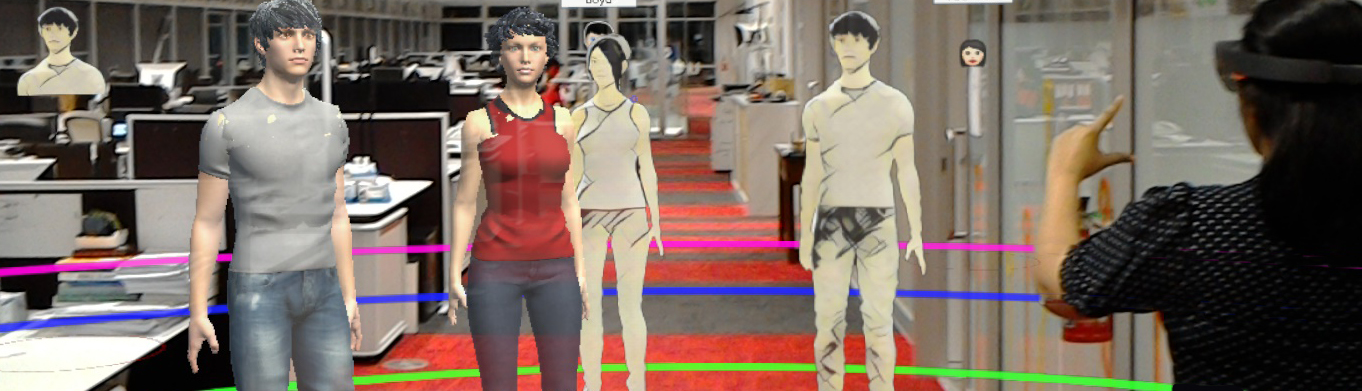
\includegraphics[width=\linewidth]{images/41-visualising-mgia17/20170618_031128_HoloLens_cropped.jpg}
  \caption{Representing social contacts in AR with different levels of proximity and visual fidelity}
  \label{fig:contacts:overview}
\end{figure}

Figure \ref{fig:contacts:system-diagram} shows an overview of the system components. The prototype uses the HoloLens Spatial Mapping feature to place virtual concentric circles (Circle Manager) on the ground around the user's initial position. On these circles, the social contacts are represented (Friend Manager) by either: a generic person silhouette, a 3D avatar, a 2D image, a bust image, or an emoji. The Scenario Manager controls the overall application, while the Friend Manager controls how friends are rendered. The Circle Manager controls the initial placement of the circles around the user. Spatial mapping is used to place circles and social contacts on the floor. Morph3D is used for rendering 3D avatars. 

\begin{figure}[h]
  \centering
  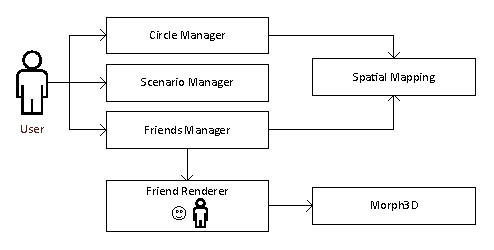
\includegraphics[width=0.8\linewidth]{images/41-visualising-mgia17/system-diagram.eps}
  \caption{System components}
    \label{fig:contacts:system-diagram}
\end{figure}

To arrange the social network, the user can use hand gestures (e.g., tap and drag) (Table \ref{tbl:contacts:gestures}) to move a virtual avatar closer or further away from the centre of the circles or change the social group the contact belongs to. The representation of the avatar automatically updates to match the selected social group. For instance, if the user selects a 3D avatar from the Intimate circle and moves it to the Friends circle, then their representation will turn into a bust image to reflect the target social group.

\begin{table}[h]
    \caption{Hand gestures used for interacting with social contacts through the HoloLens}
    \label{tbl:contacts:gestures}
    \centering
    \begin{tabular}{@{}lll@{}}
    \toprule
    Gesture      & Action                                       &  \\ \midrule
    Tap          & Select avatar                                &  \\
    Tap and hold & Move avatar between social proximity circles &  \\ \bottomrule
    \end{tabular}
\end{table}

\subsection{Focus Group Evaluation}

To evaluate the interface concept and collect feedback from potential users, this research conducted two focus group sessions with a total of 11 participants. The first group consisted of six post-graduate students working on AR/VR research. The second group was a mix of five professional visual graphics and user experience designers who have not worked on AR/VR before. Each session was divided into two activities: (1) user participatory design and (2) a usability test with the prototype. 

The focus group began with a discussion and brainstorming session on how to visualise social network contacts in an AR environment. The concept of social networking in AR was briefly introduced. A few challenges were observed, such as visual clutter, but no demonstration of the prototype system was given to avoid priming. This activity included three tasks: 

\begin{itemize}
    \item {Task 1: Imagine the future of social networks in AR. The participants were asked to draw or describe their vision of the future of how to represent social networks in AR. They then presented their ideas to the group and exchanged feedback.
    }
    
    \item {Task 2: Map social groups in terms of physical distance The participants were asked to order four different social groups (Intimate, Friend, Acquaintance, Stranger) in terms of physical distance from the user. Participants were given four silhouettes (Figure \ref{fig:contacts:silhouettes}) on paper that had one of the social groups written on the top and asked them to place them on an arrow that had four positions; closest, close, far and farthest.
\begin{figure}[ht]
    \centering
    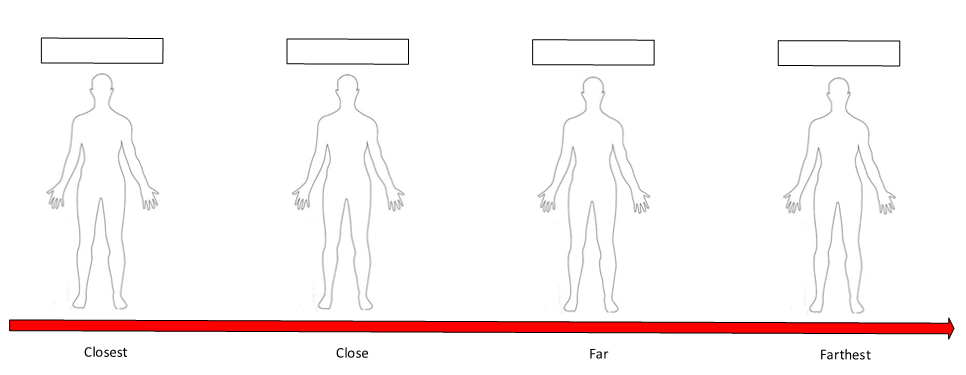
\includegraphics[width=\linewidth]{images/41-visualising-mgia17/silhouettes.PNG}
    \caption{Four placeholder for identifying the proximity of social relationships of a Friend, Strangers, Intimate, and Acquaintance}
    \label{fig:contacts:silhouettes}
\end{figure}
    }
    
    \item {Task 3: Map social groups in terms of visual fidelity. The participants were asked to match four different types of visual fidelity (3D avatar, 2D image, Bust image, Emoji) to four social groups (Intimate, Friend, Acquaintance, Stranger). This task included two sets of avatars, male and female.
\begin{figure}[ht]
    \centering
    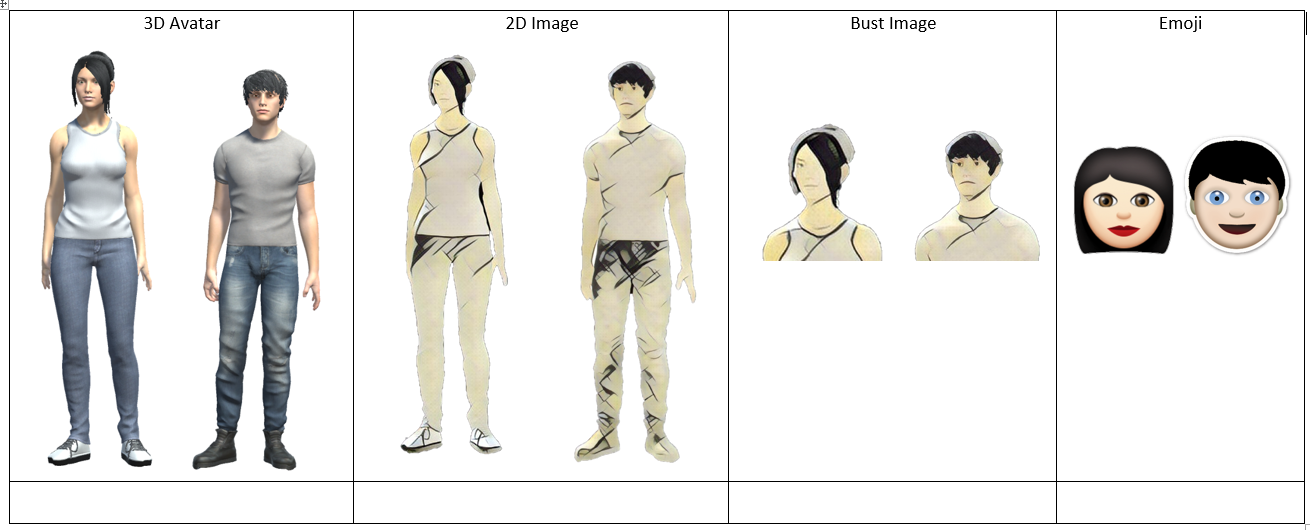
\includegraphics[width=\linewidth]{images/41-visualising-mgia17/avatars.PNG}
    \caption{Four placeholder for identifying the social relationships by an avatar representation of 3D avatar, 2D image, Bust image, Emoji}
    \label{fig:contacts:avatars}
\end{figure}    
    }
\end{itemize}

In the second session, the usability test, a demonstration was given of the prototype implementation, and the participants were asked for feedback on the following four conditions (see Figure \ref{fig:contacts:conditions}): 


\begin{itemize}
    \item{C1-Baseline (B): all avatars had the same visual representation (silhouette), and they were at the same distance away from the user.}
    
    \item{C2-Visual Proximity (P): the avatars were placed at different distances from the user based on their social intimacy (the Intimate group was the closest, then Friends, then Acquaintance, then Strangers). However, they were all a silhouette representation with the same Visual Fidelity.}
    
    \item{C3-Visual Fidelity (F): the avatars were placed at the same distance away from the viewer but had different visual representations based on their social group. The Intimate group was represented by an animated 3D avatar that moved and looked around. 2D static images represented friends, Acquaintances in 2D busts and Strangers were emojis.
    }
    \item{C4- Combined (C): both proximity and visual fidelity to filter social connections based on their social group.}

\end{itemize}

\begin{figure}[ht]
    \centering
    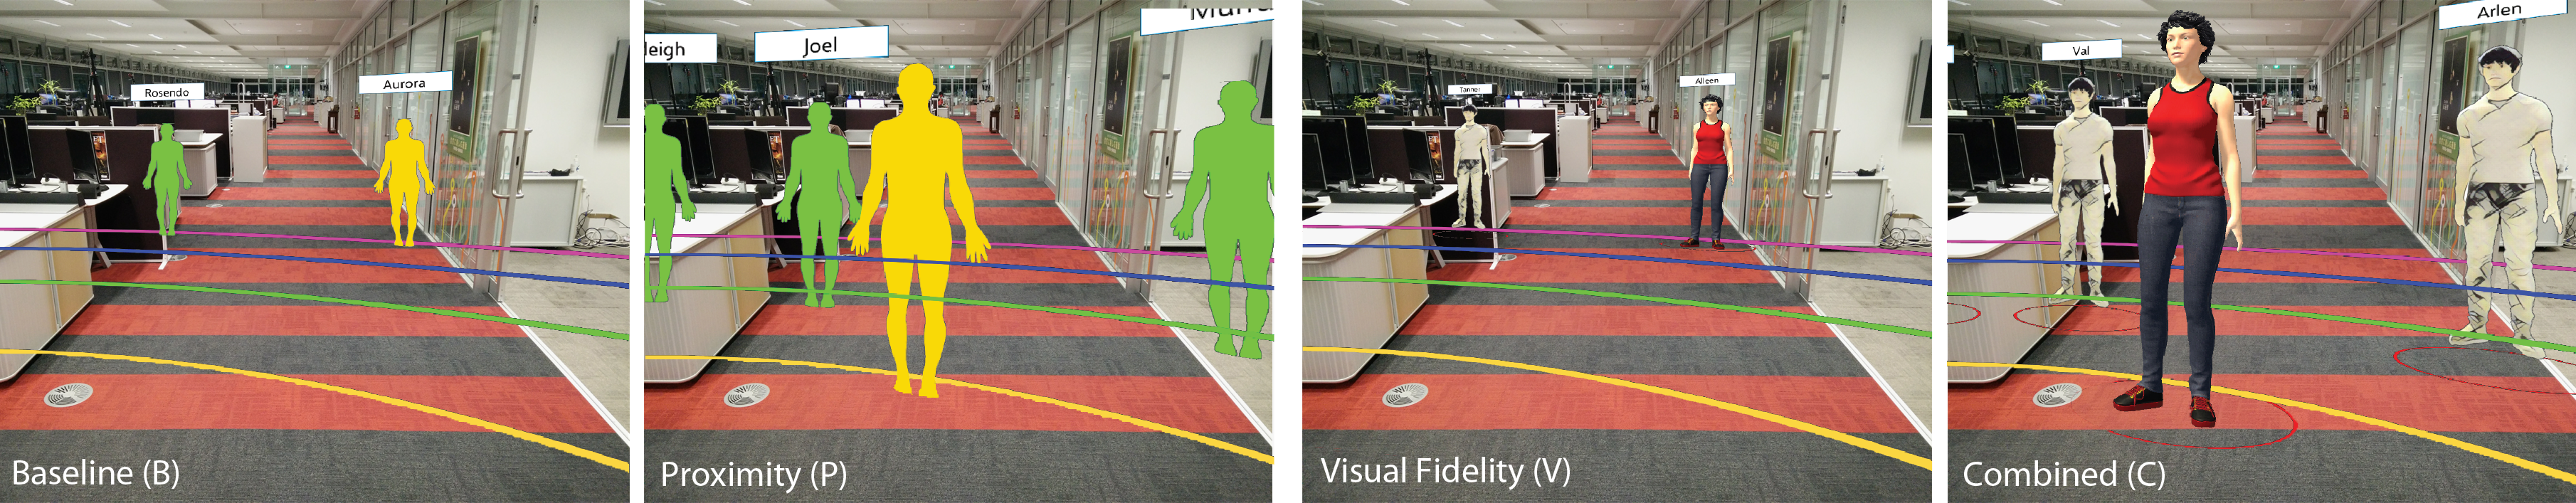
\includegraphics[width=\linewidth]{images/41-visualising-mgia17/conditions-transparent-background}
    \caption{Four conditions for representing social contacts as seen through the HoloLens. Baseline (B): fixed Visual Proximity and Visual Fidelity; Visual Proximity (P): variable Visual Proximity, but fixed Visual Fidelity; Visual Fidelity (V): same Visual Proximity, variable Visual Fidelity, and Combined (C): variable Visual Proximity and Visual Fidelity}
    \label{fig:contacts:conditions}
\end{figure}

Each participant tried the four conditions in random order, and for each condition, participants filled out a System Usability Scale (SUS) questionnaire \cite{brooke1996sus}. They also answered the following three personal questions, on a Likert scale from 1 to 7, where 1=\textit{Not very natural/easy} and 7=\textit{Very natural/easy}:

\begin{itemize}
    \item SQ1: How natural was the mapping of proximity to the social relationship?
    \item SQ2: How natural was the mapping of visual fidelity to the social relationship?
    \item SQ3: How easy was it to distinguish between the different avatar types?
\end{itemize}

\subsection{Results}

For this experiment, 11 participants were recruited, four female, aged between 16 and 41 years old, Median=29, SD=5.89. Most (85\%) used social networks (e.g., Facebook, Instagram, Snapchat) daily, and about 60\% reported using AR/VR headsets (e.g., HoloLens, HTC Vive) every month or more often. Only two people reported having no experience with AR/VR headsets before.

For \textit{Task 1}, when asked about how they would imagine representing social contacts in an AR platform, there were two main recurring themes, listed in order of popularity.

\textit{Theme 1 - Virtual Avatars}: Display virtual avatars representing friends around the users using spatial cues to distinguish them. The user can interact with other avatars to see their interests, posts or their location. The user can initiate a voice or video call with one of their contacts by interacting with the avatars.

% Mark: Did the people draw any pictures of their ideas? It would be good to include these as figures.

\textit{Theme 2 - Miniatures}: Display miniature avatars (spheres or bubbles) spread around the user environment, each bubble representing a friend. The locations of the bubbles could be determined by the social connection that the user has with that contact. Close friends could be placed near the user on a table surface while strangers are on the ground or further away. A user could pick up one of these bubbles and move them from one social group to another. The bubbles could follow the user when he moved to another place/room and re-arrange themselves according to the surrounding physical environment.

Other themes included seeing what others are seeing from their point of view, and highlighting who is online (coloured) or offline (greyed out) was also mentioned.
% Mark Billinghurst: Was there a difference between ideas suggests from HITLabNZ students and those people outside the lab?

% mark: [Do you have a list of all the 11 ideas? Maybe we can include that somehow]

% TODO (Gun): [Add a couple of sentences here (or in the discussion section) about how similar or different were the user's proposed design compared to our design (prototype system).]

For \textit{Task 2} (Figure \ref{fig:contacts:visual-fidelity}), participants were asked to order friend categories based on proximity (distance from the user). Most (90\%) participants ordered the categories as follows: Intimate, Friend, Acquaintance, Stranger on the scale from closest to furthest away from the user. This shows that users associated proximity to intimacy. Only one person chose: Intimate, Stranger, Friend, Acquaintance. 

\begin{figure}[ht]
    \centering
    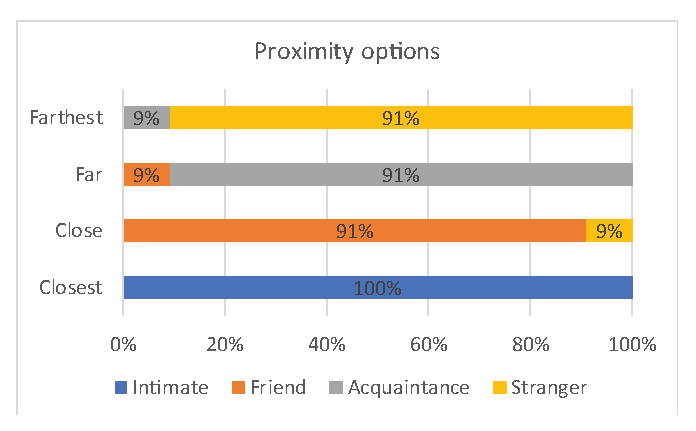
\includegraphics[width=0.8\linewidth]{images/41-visualising-mgia17/analysis-images-06.eps}
    \caption{Visual Fidelity categorisation for social contacts}
    \label{fig:contacts:visual-fidelity}
\end{figure}

For \textit{Task 3} (Figure \ref{fig:contacts:proximity}), participants were asked to categorise four types of visual fidelity. Most participants (73\%) associated 3D avatars with an Intimate relationship, 59\% marked the 2D image as a  Friend, 64\% associated the bust image for Acquaintances, while 45\% marked Emoji for Strangers. 14\% assigned 3D avatar with Stranger, a 2D image with Acquaintance, Bust images with Friend and Emoji with Intimate. 

% mark: In the discussion section, you might want to talk about the outliers
% mark: Maybe put this as a table?
% TODO (Gun): [Add here (or in the discussion section) how the results align with (or different from) our proposed design of the prototype system].
% mark: [It would be good to include comments from the users as to why they organised them in this way]

\begin{figure}[ht]
    \centering
    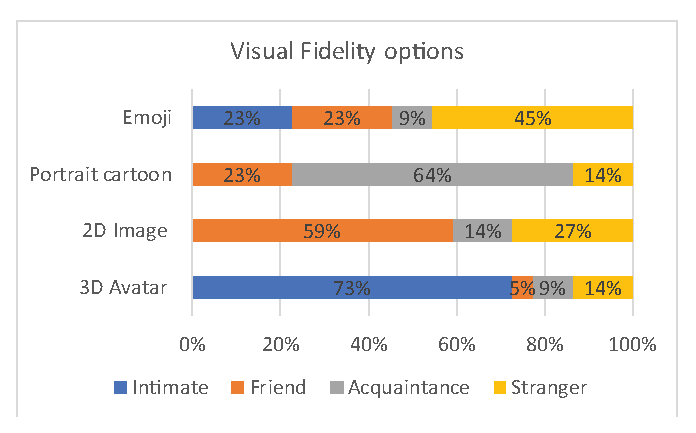
\includegraphics[width=0.8\linewidth]{images/41-visualising-mgia17/analysis-images-01.eps}
    \caption{Proximity categorisation for social contacts}
    \label{fig:contacts:proximity}
\end{figure}

The SUS scores (Figure \ref{fig:contacts:sus}) found that conditions C2-Proximity (69), C3-Visual Fidelity (69) and C4-Combined (72) were rated "Good" while C1-Baseline was "OK" (67). Data were tested for normality using Shapiro-Wilk test and found to be normally distributed ($p=0.83, 0.779, 0.292, 0.188$ for C1, C2, C3 and C4). To see if this difference was statistically significant, aligned rank transform was run on the SUS results in order to run a 2-way repeated measure ANOVA analysis with two factors Proximity and Visual Fidelity. No significant differences ($F(1, 10)=1.414,p=0.262$) were found in terms of SUS between Proximity and Visual Fidelity. 

\begin{figure}[ht]
    \centering
    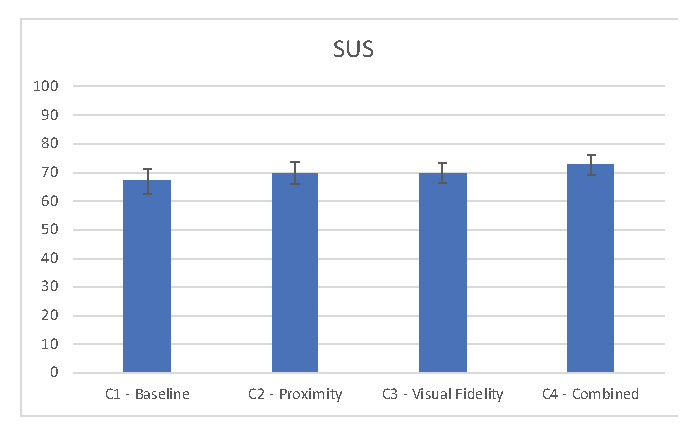
\includegraphics[width=0.8\linewidth]{images/41-visualising-mgia17/analysis-images-02.eps}
    \caption{The System Usability Score. Whiskers indicate standard error.}
    \label{fig:contacts:sus}
\end{figure}
% TODO (Gun): In the figure caption, you should mention what does the whiskers (error bars) represent. BTW, based on the error bars seems you might have had significant results? Any inferential statistics to report here? I would suggest running Aligned Rank Transform Repeated-measure two-way ANOVA. 
% mark: You should label them B, P, F and C

The subjective questionnaire (Figure \ref{fig:contacts:sq2}) shows an increase in how natural people felt the mapping to proximity (SQ1) was in the Proximity condition. A Friedman test was run and found that there was a statistically significant difference in rating the four conditions, ($\chi^2(2)=18.402,p<0.001$). Post hoc analyses with Wilcoxon signed-rank tests were conducted with a Bonferroni correction applied, resulting in a significance level set at ($alpha=0.008$). There was a significant difference between conditions C4-Combined and C1-Baseline ($Z=-2.687, p=0.007$). However, there were no statistically significant differences between the other conditions.

Similarly, there was an increase in how natural people felt the mapping to visual fidelity (SQ2) was in the Visual Fidelity condition. Running a Friedman test found that there was a statistically significant difference in rating the four conditions, ($\chi^2(2)=21.194,p<0.001$). Post hoc analyses with Wilcoxon signed-rank tests were conducted with a Bonferroni correction applied, resulting in a significance level set at $alpha=0.008$. There were significant differences between conditions C3-Visual Fidelity and C1-Baseline ($Z=-2.825, p=0.005$) and between conditions C4-Combined and C1-Baseline ($Z=-2.820, p=0.005$). However, there were no statistically significant differences between the other conditions.

As for the (SQ3), people felt it was easier to distinguish between different avatars in both the Visual Fidelity and Combined conditions. Running a Friedman test found that there was a statistically significant difference in rating the four conditions, ($\chi^2(2)=20.967,p<0.001$). Post hoc analyses with Wilcoxon signed-rank tests were conducted with a Bonferroni correction applied, resulting in a significance level set at $alpha=0.008$. There were significant differences between conditions C3-Visual Fidelity and C1-Baseline ($Z=-2.816, p=0.005$) and between conditions C4-Combined and C1-Baseline ($Z=-2.829, p=0.005$). However, there were no statistically significant differences between the other conditions.


\begin{figure}[ht]
    \centering
    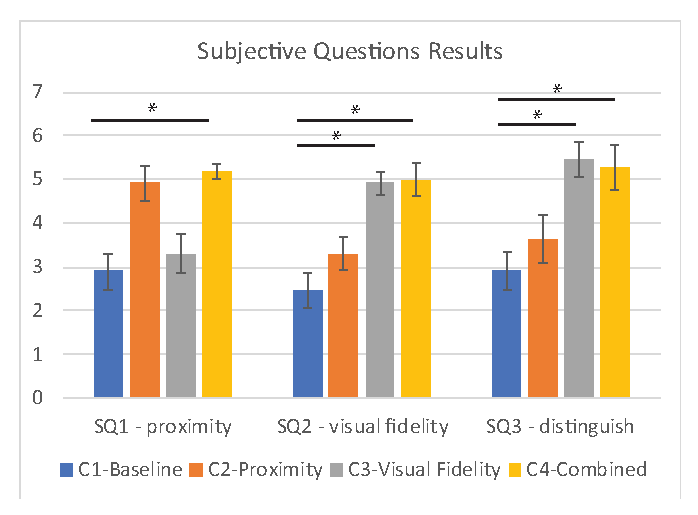
\includegraphics[width=0.8\linewidth]{images/41-visualising-mgia17/analysis-images-05.eps}
    \caption{Subjective question results by condition by question. Whiskers indicate standard error. *=statistically significant difference}
    \label{fig:contacts:sq2}
\end{figure}

For ranking the conditions (Figure \ref{fig:contacts:ranking}), participants ranked the four conditions from 4 to 1, where four was the most preferred and one the least preferred. Results show that participants preferred conditions C3-Visual Fidelity and C4-Combined over C2-Proximity and C1-Baseline. A Friedman test found that there was a statistically significant difference in ranking the four conditions ($\chi^2(2)=15.222,p=0.002$). Post hoc analyses with Wilcoxon signed-rank tests were conducted with a Bonferroni correction applied, resulting in a significance level set at $alpha=0.008$. There was a significant difference between C3-Visual Fidelity and C1-Baseline ($Z=-3.035, p=0.002$). However, there were no statistically significant differences between the other conditions.

\begin{figure}[ht]
    \centering
    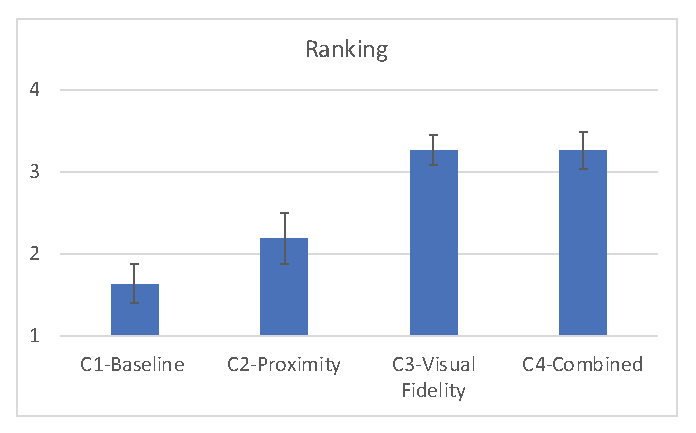
\includegraphics[width=0.8\linewidth]{images/41-visualising-mgia17/analysis-images-04.eps}
    \caption{Ranking (4=highest, 1=lowest). Whiskers indicate standard error.}
    \label{fig:contacts:ranking}
\end{figure}

\subsection{Discussion}

The user study results found that subjects preferred having a filter to represent their social contacts rather than no filter (i.e., Baseline condition). Based on the ranking results, the most preferred filters are the Visual Fidelity and Combined filters, followed by the Proximity filter.
% TODO (Gun) : [Discuss how this is similar to our proposed design or what is the difference? How this would affect further development/design of the social AR interface?]
The subjective questions revealed that each condition was representing the natural mapping/filter of the user's social contacts (i.e., "SQ1-how natural the proximity" scored high in "P" and so on). Participants felt that the Visual Fidelity condition (V) was the easiest for distinguishing avatars.

In terms of the strengths and weaknesses of each condition, participants did not like the Baseline condition because they could not easily distinguish the avatars. For example, one participant said, "\textit{I cannot distinguish avatar so well, I do not want to look around at everyone at the same distance}". This confirms our original predictions regarding the placing of social contacts.

With the Proximity condition, participants reported positive feedback and an increase in avatar presence, but they were not able to adequately distinguish users from each other.  One user said "\textit{I feel more spatial presence}", but another said "\textit{I need to look around more to see what is where.}"

In the Visual Fidelity condition, participants reported that it was easy to distinguish between contacts, but the interface could be improved. One user said "\textit{This one felt more comfortable with people at a distance and was easy to tell people apart}", while another user said, "\textit{Take more visual space for people whom I do not want to interact with.}"

For the Combined condition, participants reported it was the best because they felt that it was easier to distinguish between avatars. One user said "\textit{More info is available (fidelity + distance)..}".
However, some participants did not like it when the avatars were too close and recommended increasing the minimum distance between the user and the closest circle.

The limitations of this work include that the avatars are not a true representation of the participants' social contacts. This study assumes a predefined set of social contacts mixed between male and female and different outfits. This system assumes four levels of social relationships: 1) intimate, 2) friend, 3) acquaintance and 4) stranger. Users may have fewer or more levels of social contacts. 

Overall, the results confirmed our hypothesis that users would prefer to have their social contacts filtered out based on their relationship to them. The question was which filter (Proximity or Visual Fidelity) is best for each condition. Users seem to prefer either visual fidelity or a combination of visual fidelity and proximity. This may remain a user preference. 

% Tobias: You do not discuss shortcomings/limitations of the study (e.g. internal and external validity). This should all come into the discussion sections, which is missing, as stated before.

\subsection{Conclusions}

This section investigated different visualisation options for representing social contacts in a wearable AR interface. Two focus groups were conducted to get feedback from potential users about how they would want to organise social contacts in an AR interface. Participants identified visual representation and spatial cues as common ways to do this. This matched the interface metaphor used to develop a working prototype.

The user study measured the usability and user preference of four conditions in a prototype AR interface on a HoloLens display: 1) Baseline, 2) Proximity, 3) Visual Fidelity and 4) Combined. Participants indicated that it was useful to have some different visual fidelity representations of their AR social contacts and that combined use of visual fidelity and proximity was also useful. These conditions highlight the dimension of representing social contacts on the Social AR Continuum. The next section looks into the dimension of placing social contacts. 

% In the future, we plan to explore and further develop different visual fidelity representations of social contacts (e.g., displaying avatars as miniatures on a nearby surface). We will also investigate different ways to interact with other users in social networks who are either physically collocated or remote.

%checked by mark May 9th 2019
\pagebreak
\section{Placement of Social Contacts}
\label{sec:contacts:placing}

This section looks into options of where to place social contacts relative to the user \cite{Nassani2017a} by testing two options (Figure \ref{fig:continuum:conditions}): 1) Life-sized, where social contacts are presented as human-size virtual avatars displayed around the viewer, and 2) Miniature, where the social contacts are displayed on a table-top nearby the viewer. 

\begin{figure}[ht]
    \centering
    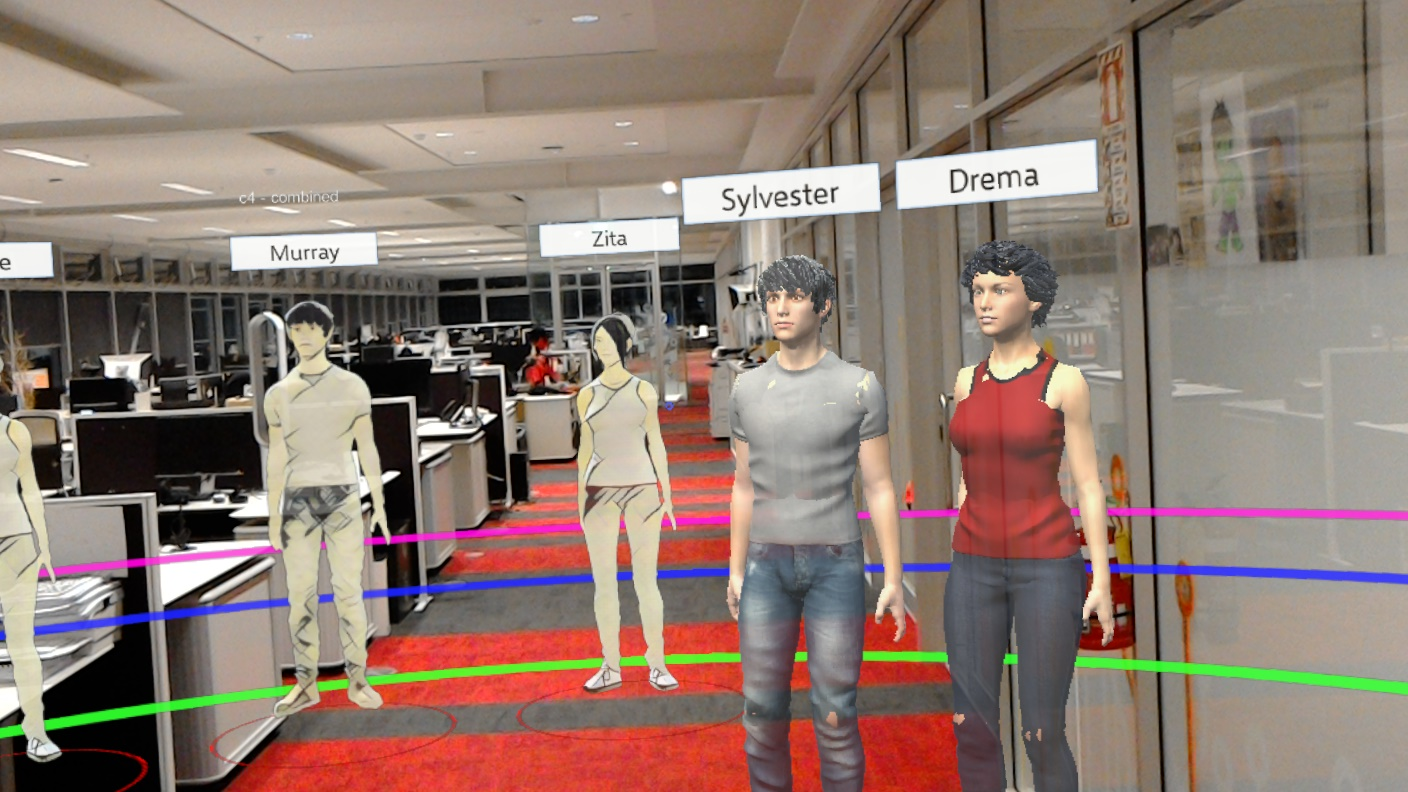
\includegraphics[width=0.8\linewidth]{images/42-placement-ismar17/20170625_205203_HoloLens.jpg}    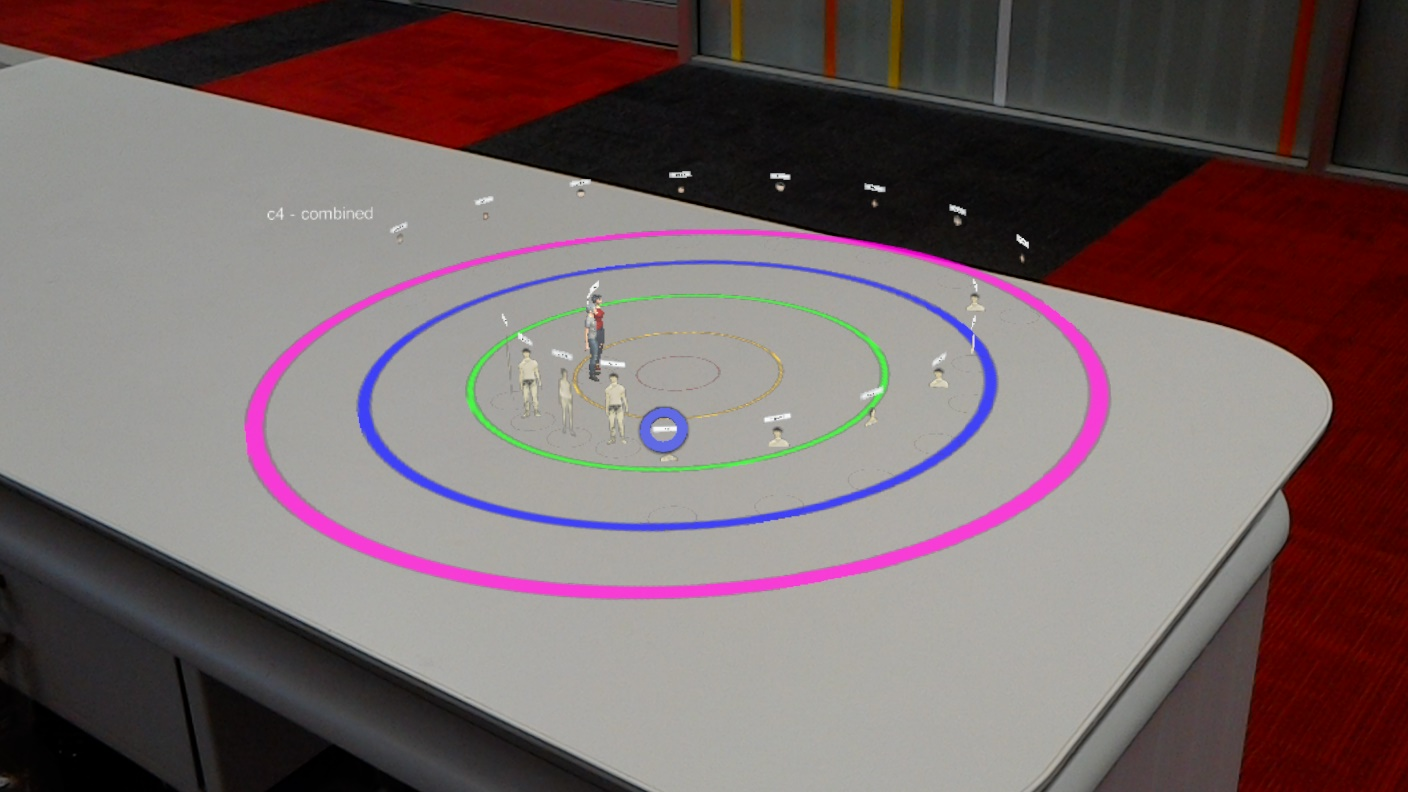
\includegraphics[width=0.8\linewidth]{images/42-placement-ismar17/20170625_205112_HoloLens.jpg}
    \caption{Prototype interfaces for contact placement. Life-sized (top) on the ground vs. Miniature (bottom) on a nearby surface.} 
    \label{fig:continuum:conditions}
\end{figure}

\subsection{Implementation}

A prototype was implemented (Figure \ref{fig:placement:system}) on the Microsoft HoloLens to test the two conditions on the contact placement dimension, one viewing avatars. The prototype also allowed the user (as a viewer) to select and move an avatar closer to or further away from the viewer position by using air-tap gestures of the HoloLens. The air-tap gesture\footnote{https://docs.microsoft.com/en-us/windows/mixed-reality/gestures} is recognised by touching the index and thumb fingers to select. The purpose of the selection and movement process was to change the social relationship between the viewer and their social contacts. When the viewer focuses on a social contact and uses the air-tap gesture, then the social contact will be able to moved from the current social proximity ciricle (e.g., Friend) to the next one (e.g. Intimate). 

\begin{figure}[ht]
    \centering
    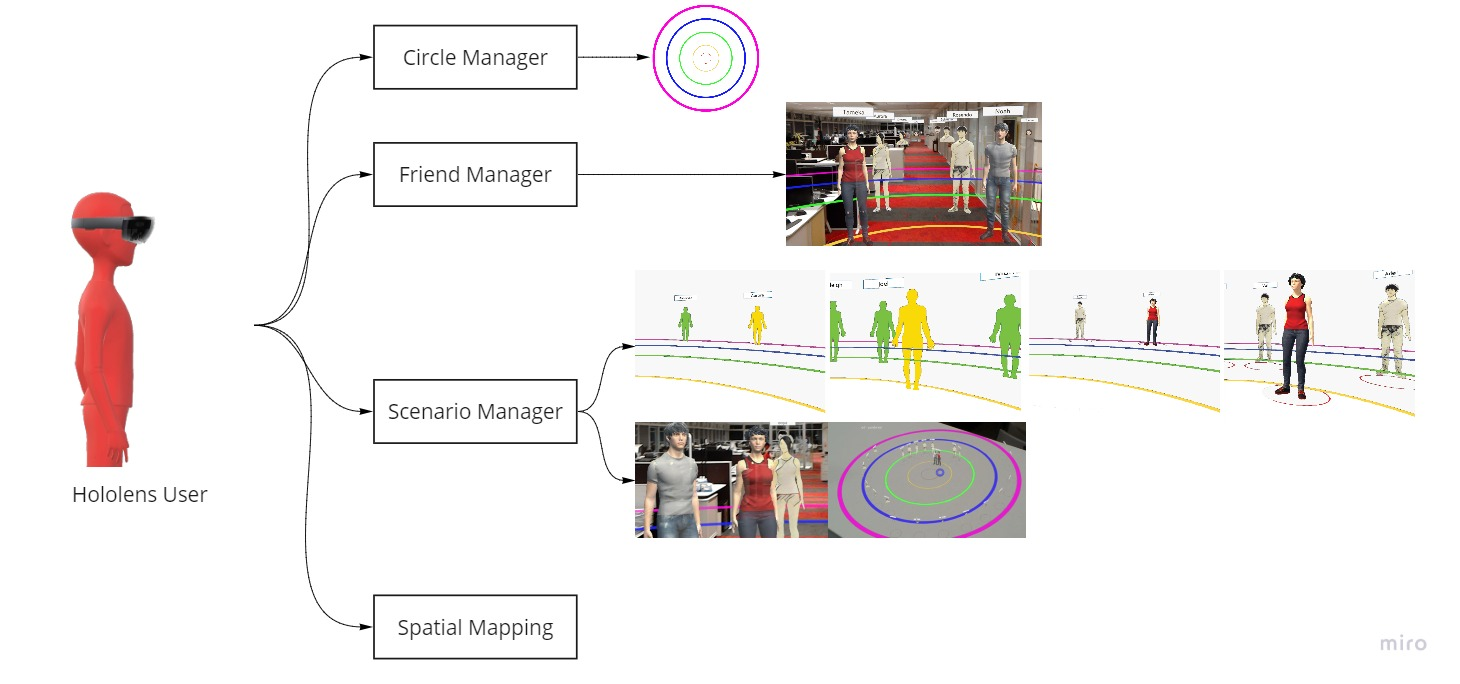
\includegraphics[width=\linewidth]{images/42-placement-ismar17/placement-system.jpg}   
    \caption{System implementation of social contacts placement on a HoloLens device} 
    \label{fig:placement:system}
\end{figure}


\subsection{User Study}

Feedback was collected from potential users during an open day at our lab as the participants tried demonstrations of the two conditions: C1-Life-sized (L) and C2-Miniature (M) representations of avatars. Twenty-seven participants (mix gender and background - unfortunately no demographics data collected for this user study) from the public  tried the system prototype. On trying a demonstration of each condition, participants were asked to rate their experience on a 7-point Likert scale (where 1=not very and 7=very) for three subjective questions on: 

\begin{itemize}
    \item Q1: How easy was it to visualise social contacts?
    \item Q2: How natural was moving social contacts?
    \item Q3: How useful was this condition?
\end{itemize}

Participants were asked to think of situations where it would be positive and negative in using each condition. Then they were asked to choose one of the conditions as their preferred condition based on their experience.

\subsection{Results}

A Shapiro-Wilk Normality Test on the questionnaire results (n=27) (Figure \ref{fig:continuum:results}) showed that the data is normally distributed ($p=0.13$). Wilcoxon signed-rank tests were run on the results of the questions but did not show any statistically significant differences between C1-Life-sized and C2-Miniature and it did not elicit a statistically significant change in Ease of Use ($Z=-0.529, p=0.597$), Natural Interaction ($Z=-1.616, p=0.106$), nor Usefulness ($Z=-1.664, p=0.096$). Participants were asked to rank the two conditions in terms of preference. The ranking results did not show any statistically significant change in ranking between conditions ($Z=-.577, p=0.564$) in a Wilcoxon signed-rank test.

\begin{figure}[ht]
    \centering
    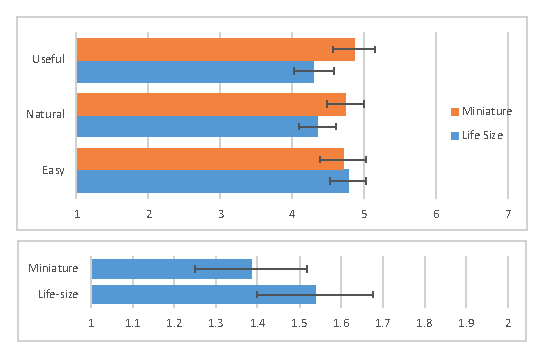
\includegraphics[width=0.8\linewidth]{images/42-placement-ismar17/images-09.eps}
    \caption{\textit{Top:} Mean values results of subjective questions grouped by condition by question. \textit{Bottom:} average ranking results of preferred condition between Life-size and Miniature; 1=most preferred, 2=least preferred. Whiskers indicate standard error.}
    \label{fig:continuum:results}
\end{figure}

Participants answered open-ended questions about the positives and negatives of each condition. Participants reported the most useful scenarios for the C1-Life-sized condition as:

\begin{itemize}
    \item \enquote{face-to-face conversations with a social contact}
    \item \enquote{when zooming into a subset group of friends}. 
\end{itemize}

Some of the positive feedback of C1-Life-sized include:

\begin{itemize}
    \item \enquote{Felt very personal, and I felt more engaged because I was actually in the situation}
    \item \enquote{Very satisfying seeing friends further out in lower fidelity. Give a real sense of good friends vs acquaintances}
\end{itemize}

While some of the negative comments on C1-Life-sized include:

\begin{itemize}
    \item \enquote{Hard to see people in the context of each other}
    \item \enquote{It was hard to get an overall perspective of all friends}
\end{itemize}
 
For the Miniature condition, participants reported this condition as useful for: 

\begin{itemize}
    \item \enquote{seeing the overall picture of social contacts} 
    \item \enquote{moving contacts between different social circles} 
\end{itemize}

Some of the positive feedback of C1-Life-sized include:

\begin{itemize}
    \item \enquote{I prefer the miniature version because I can see the whole "play space" at once}
    \item \enquote{Much better than life size to be able to see them all at once, see the big picture. Context of people relative to each other}
\end{itemize}

While others mentioned the followings as negative feedback: 

\begin{itemize}
    \item \enquote{It felt more disconnected compared to the life-size due to my position feeling further away}
    \item \enquote{Hard to select characters. Difficult to see [who is who]}
\end{itemize}

\subsection{Discussion}
% It would be good to include more discussion about the results from this user test

% Mark: It would be good to include more discussion about the results from this pilot test

% gogo: I agree. This section seems very short compared to the previous one. Also, what is the takeaway message from this section? As far as I can tell, the user preferred the miniature one, if any. Is that the one you decided to explore further? If not, why not?

% Tobias: I am missing the discussion of the insights and the directions for future work. In particular, I am missing discussions on relevance. All this should come after the results. Normally, a longer paper/thesis would have a results section which focuses on the statistical analysis but not discussion/interpretation. This is usually followed up with a discussion section which expands then on the results by offering a discussion and interpretation of these results. What do these results mean? What is the practical meaning and relevance? This section and this detailed interpretation are missing even though it is the most important. Similarly, the relevance for future work and the field of AR is missing.

The Likert scale results did not show any significant results between C1-Life-sized and C2-Miniature representation of avatars in terms of usefulness, natural or easy interactions. This indicates that both representations are valid options and depending on the use-case scenario, viewers could either see their social contacts in C1-Life-sized or C2-Miniature. There are both advantages and disadvantages for each condition drawn from the positive and negative feedback by participants. The semi-structured interview highlighted some of the positive and negative sides of each condition. This indicates that it might be ideal if the system allows for easy switching between Life-sized and Miniature placement based on the required scenarios. 


\subsection{Conclusion}

This section investigated different options of placing the social contacts; either as Life-sized avatars or as Miniature avatars. Results (Figure \ref{fig:continuum:results}) showed that participants did not have any preference between the life-size condition and the Miniature condition, and it is a matter of user preference. Therefore, in the next chapters, we focus on displaying social contact as Life-Sized.


\section{Summary}
%You should add a summary section to the overall chapter discussing how these studies helped to answer the research question

This chapter explored different options of visualising social contacts on AR devices.

\todo[inline]{add more}

\chapter{Social Data in AR} 
\label{ch:data} 

This chapter addresses the shared social data and surrounding environment of the user in terms of the Social AR Continuum. The level of detail can be determined based on the relationship between the user and the social contact with whom they are sharing the data and surrounding environment. The aim of this chapter is to answer the research question \ref{rq:data}: \textit{What is the best way to view and interact with shared social data on wearable AR displays?}. 

% Gun: You may potentially categorise this in a higher level concepts. For example, changing the type of representation (2D photo, 360 photo, 3D ..), spatial parts/amount of representation, and the level of detail (e.g. resolution) of representation. You may want to update the section titles accordingly.

This chapter studies: 1) different types of representing shared social data (e.g., 2D photo, 360-degrees images, and 3D surrounding environment) \ref{sec:surrounding:360}, 2) different level of detail of shared 3D surrounding environments \ref{sec:surrounding:environment}, and 3) 

This chapter studies two different ways of sharing the surround environment (360 Panoramas \ref{sec:surrounding:360}, 3D Scanned Surroundings \ref{sec:surrounding:environment}). Additionally, this chapter looks into partially sharing/hiding \ref{sec:surrounding:hiding} part of the environment with social contacts, based on privacy concerns. For each way of sharing, this chapter discusses the levels of detail that can be shared based on the user relationships. 

\section{Filtering Shared Social Data}
\label{sec:surrounding:360}

The social data of the surrounding scene can be described in different levels of detail. A different ways of describing a surrounding scene include: a 2D image, a panoramic image, a video, a 360-degrees video, a 3D depth image, or a VR 3D model. These different ways of describing the same scene represent the levels of details that can be varied based on the Social AR Continuum and the social proximity between the social contacts. 

This section describes a method and a prototype implementation for filtering shared social data (e.g., 360-degree videos) using wearable AR devices (e.g., HoloLens) \cite{Nassani2018a}. The data filtering is based on the sharer-viewer relationships in order to preserve privacy. For example, when sharing a 360-degrees video, if the user has an intimate relationship with the viewer, then the full fidelity (i.e., the whole 360-degree video) of the sharer's environment is visible. However, if the two are strangers, then only a snapshot image is shared, and the viewer cannot get more information about the sharer's environment. By varying the fidelity of the shared content, the viewer can focus more on the data shared by their close (in terms of social proximity) relations and differentiate this from other content. Also, this approach enables the sharer to have more control over the fidelity of the content shared with their contacts for privacy.

% In this work, we are trying to answer the question, what would be the best way to share rich data (such as 360 videos) within a large social network? The hypothesis is that filtering data based on the user-viewer relationship or proximity will increase the feeling of being together or inter-connectedness. 


% =============================================================================
\subsection{Sharing Social Data}
% =============================================================================

From the perspective of the person who is sharing the data (the sharer) with their social contacts (Figure \ref{fig:data:sharer}), the data is collected in its highest fidelity (e.g., a fully spherical 360-degree view) which will be shared with those viewers with the closest (most intimate) social relationships. For less-intimate friends, a 2D video, extracted from the 360 videos based on the sharer's view direction over time, will be shared. For Strangers, the sharer can select which snapshot image from the 2D video sequence to display. The central metaphor is that the closer the relationship that the user has to the viewer, the richer data that they can share from their point of view (360-degree videos, 2D videos, still images).

\begin{figure}[ht]
    \centering
    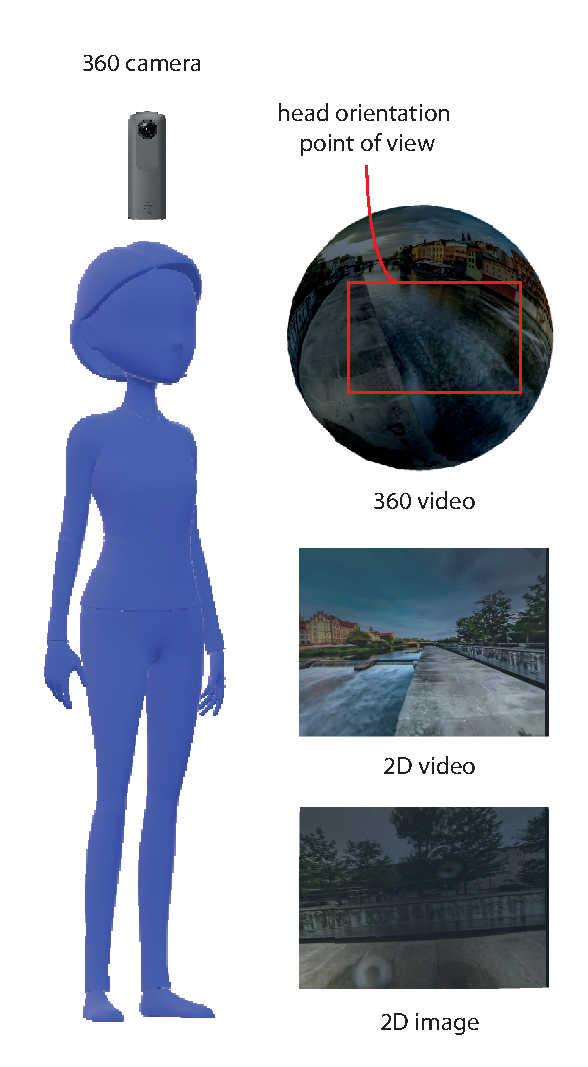
\includegraphics[width=.8\linewidth]{images/chi/images-04.eps}
    \caption{Sharing point of view with different fidelity of representation.}
    \label{fig:data:sharer}
\end{figure}

An example use-case scenario for filtering by sharer is where the sharer is going on a hike and wanting to share the experience of being in an interesting place such as near a river. The sharer takes a live 360-degree video of the surrounding environment and shares it with her followers. The sharer then gets to see how the followers are able to see the shared data based on their social relationship to her. The sharer's intimate friends and family will see the live 360-degree video, other friends the 2D video, and strangers still images of the scene, all automatically created from the 360-degree video recording.

% =============================================================================
\subsection{Viewing Shared Social Data}
% =============================================================================

The user viewing the shared data (the viewer) uses a wearable AR interface to see content from their social network superimposed over the real world, based on proxemics. For example, the viewer may be interested in seeing what their social contacts (followers) are up to and the places they have been. In this scenario the viewer can look around through the AR display to see their social contacts placed around them in three circles ordered by relationship. On top of each social contact, the viewer can see the content they are sharing, filtered based on the social relationship between the social contact and the viewer.

Based on our earlier work of representing social contacts \cite{Nassani2017a}, the people who are socially closer will appear in the AR view visually closer and have a more realistic representation. The content shared by each social contact will appear above their avatar (see Figure \ref{fig:data:viewer}), and to view the content more clearly, the user can select it (e.g., using the HoloLens air-tap gesture) to bring the content closer or walk to move inside the 360-degree video sphere. The user can then tap again to bring back the content to its original place to see other social contacts. 

\begin{figure}[ht]
    \centering
    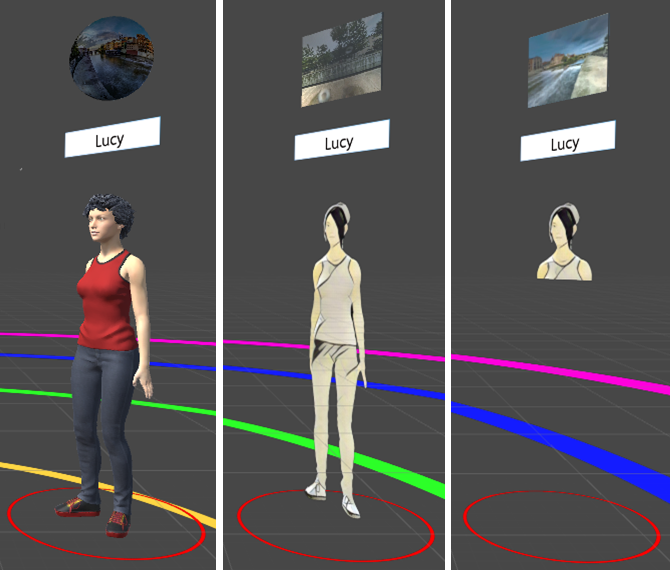
\includegraphics[width=3in]{images/chi/3_levels_of_data.png}
    \caption{Social contact sharing in different relationships with the viewer (Left to right: Intimate, Friend, Stranger). The shared data content (above the avatar) is filtered (360-degree video, 2D video, 2D image) based on social relationship.}
      \label{fig:data:viewer}
\end{figure}

In addition to this operation, this section proposes that the viewers can also see the shared content in different fidelity (360-degree videos, 2D videos or images) based on the social relationship with the sharer (Intimate, Friend or Stranger). While the sharer could restrict the fidelity of the shared content based on the social relationship as mentioned earlier, the viewer could also filter the content based on their preference. In order to avoid getting mentally overloaded by seeing too much content in high fidelity, the viewer should be able to choose the preferred fidelity for the shared content from each social contact. This could be achieved either explicitly by choosing a fidelity for each social contact, or implicitly by moving closer to or further from the avatar representing the contact.      

% =============================================================================
\subsection{Prototype}
% =============================================================================

To explore using the Social AR Continuum metaphor for sharing data between social contacts, a prototype was built using the Microsoft HoloLens. The prototype software was built using Unity 3D game engine, and it allows users to view their social contacts on a wearable AR interface. Figure \ref{fig:data:system} shows the structure of the prototype system. 

\begin{figure}[ht]
    \centering
    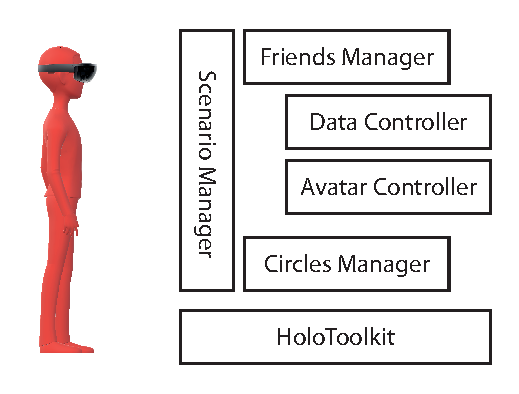
\includegraphics[width=3in]{images/chi/images-03.eps}
    \caption{System components.}
    \label{fig:data:system}
\end{figure}

The prototype places social contacts around the user (viewer) in three concentric circles which are controlled by the \textit{Circles Manager}. The social contacts have different visual fidelity and proximity based on their initial relationship to the viewer, and are rendered using the \textit{Avatar Controller}. The avatars were randomly pre-generated without any resemblance to actual contacts. MakeHuman\footnote{http://www.makehuman.org/} was used to generate the 3D avatars. The viewer (HoloLens user) can turn their head to face different social contacts and then use gestures (air taps) to interact with the contact (view their data or change their position which represents the social relationship). The interactions with HoloLens are enabled using the open-source library \textit{HoloToolkit}\footnote{https://github.com/Microsoft/MixedRealityToolkit-Unity}. The data content shared by the social contacts are controlled by the \textit{Data Controller} which determines which fidelity needs to be displayed based on the social relationship between the avatar and the viewer. The top-level \textit{Scenario Manager} defines the implementation needed for different conditions in the user study, including interaction with avatars, shared data and the concentric circles. 

% =============================================================================
\subsection{User Study}
% =============================================================================

A user study was conducted to test the system usability and effects on social presence, comparing the following conditions: 

\begin{itemize}
    \item C1) Baseline: Shows the shared 360-degree videos from all social contacts.
    \item C2) Tap-to-change: Filters the fidelity of the shared 360-degree videos based on the relationship between the viewer and the social contact. The user can tap on any social contact to cycle through different relationships.
    \item C3) Walk-to-change: Filter the fidelity of the shared 360-degree videos based on the physical distance between the viewer and the social contact.
\end{itemize}

The task was for participants to wear the headset and observe 12 social contacts (mocked up, not reflecting the participant's real social contacts) placed around the user at equal angles from each other to complete a circle (360 degrees) around the viewer, and at different distances to the viewer (centre) based on the social relationship. Each social contact had shared content floating above their head, filtered depending on the type of social relationship that the social contact had with the viewer. 

The participant could view the data content by performing the air-tap gesture on it. Once tapped, the content moved closer to the viewer. For instance, if the viewer tapped on the sphere of a 360-degree video, then the sphere immersed the participant to experience it, while for a 2D video, it was moved closer to the user so they could see it at full-screen resolution.

Participants were asked to answer the 5-point Likert-scale questions shown in Table \ref{tbl:questions} which are based on prior work \cite{Biocca2003}. Participants were asked to rate their experience on the Subjective Mental Effort Questionnaire (SMEQ) \cite{Sauro2009}. 

\begin{figure}[ht]
    \centering
    \includegraphics[width=1.5in]{images/chi/images-02.eps}
    \caption{Questionnaires for Social Presence including the following dimensions: CoPresence (CoP), Attentional Allocation (Atn), Perceived Message Understanding (MsgU). *=negative} 
      \label{tbl:questions}
\end{figure}

% =============================================================================
\subsection{Results}
% =============================================================================

A user study was run with eight participants (four female) aged 26-35 (SD=3.03). All participants used social networking platforms on a regular basis, and most (How many?) were familiar with AR/VR displays. 

After filling in a demographic questionnaire, the participants were asked to experience the three conditions in random order. Then they filled in a social presence questionnaire and SMEQ about the condition they just tried. After finishing all three conditions, participants then filled in a post-experiment questionnaire where they were asked about the overall experience and if they had any suggestions to improve it. 

From the questionnaire results (Figure \ref{fig:data:results}), indicates that C2 was rated (3.6) better in terms of social presence compared to C1 (3.3) on average, while C3 (3.5) was relatively close compared to C2. The SMEQ results show that all three conditions were rated low in terms of mental effort, while both C2 (M=16.875) and C3 (M=16.875) were rated lower than C1 (M=21).

\begin{figure}[h]
  \centering
  \includegraphics[width=\columnwidth]{images/chi/images-01.eps}
  \caption{Results of social presence (top) and SMEQ (bottom). *=reversed rating scale. Whiskers=standard error}
  \label{fig:data:results}
\end{figure}

As part of the post-questionnaire, participants were asked to rate the three conditions (1=least preferred, 3=most preferred). The ranking results (see Figure \ref{fig:data:ranking}) show that C1 was least preferred (1.3) while C2 (2.25) and C3 (2.375) were similar. There was a statistically significant difference in ranking conditions $\chi^2(2)=7, p=0.05$. A post-hoc analysis with Wilcoxon signed-rank tests was conducted, finding a statistically significant difference between C1-baseline and C3-Walk to change. ($Z=-2.081, p=0.037$), and no difference between the other conditions.

\begin{figure}[h]
  \centering
  \includegraphics[width=1.5in]{images/chi/images-05.eps}
  \caption{Condition ranking results. Reverse rating scale: 1=least preferred, 3=most preferred. Whiskers=standard error. $*=$ statistically significant difference (Friedman test: $X^2(2)=7, p<0.05$).}  
      \label{fig:data:ranking}
\end{figure}

% =============================================================================
\subsection{Discussion}
% =============================================================================

From a semi-structured interview after the experiment, most users found that condition C3 (walk to change) was a more fun and natural way to view shared data from social contacts. "I feel it is more real and fun to view the 360 videos by walking toward the avatar". Also, other subjects found that the walking condition was more suitable for an outdoor or open area to avoid running into obstacles while walking. The condition C2 (tap to change) was found more convenient for changing the relationship rather than requiring more physical effort, such as walking. The Baseline condition (C1) was the least favourite for participants, as it was too overwhelming having all 360-degree videos shown all around. 

On the downside, participants mentioned some weakness for condition C2 (tap to change), such as potential clutter by being able to bring all social contacts into a small area of the intimate circle. While condition C3 (walk to change) did not have that issue, it was mentioned that by walking one might accidentally change the relationship with other social contacts that the user was not focusing on. For example, the avatars behind or on either side of the user would be affected by user movement, even if the user did not intend to get close to them. Viewing 360-degree videos through an optical see-through display was considered not as ideal, as the 360-degree videos appear to be semi-transparent on top of the real environment.

Overall, participants expressed their interest in using such a system to manage and view their social contacts and shared content in AR, and that it would be useful and easy to use. 

% =============================================================================
\subsection{Limitations and Future Work}
% =============================================================================

This prototype used asynchronous sharing, where social contacts were not online at the same time, sharing live data; the shared content was previously prepared, and the 360-degree videos were previously processed to extract 2D video and a 2D image. However, the method was applied for filtering could be applied to synchronous sharing as well. In the future, the plan is to add live video streaming from social contacts and live scaling down of the content based on social relationships. 

% The concept does apply to synchronous sharing where social contacts are online at the same time. Future plans includes extending this prototype for synchronous sharing experiences. We can expand the implementation to include spatial audio as a fidelity option on which to filter based on social relationship. 

% Additionally, we will conduct a full quantitative and qualitative user study to measure the effects of filtering content type on social presence and user experience. 

% =============================================================================
\subsection{Conclusions}
% =============================================================================

This section presented a mechanism for presenting shared data content by filtering the content type based on the social relationships between the user and the social contacts. 

This work includ an implementation on HoloLens prototype for applying the proposed method in an asynchronous collaboration scenario and conducted a user study using the prototype. The study compared three conditions: viewing 360-degree video without filtering, filtering based on the social relationship, and filtering based on distance.

Initial results showed a trend of participants favouring having the option to filter data over not filtering. The results included a qualitative feedback that provides insights for future directions. 

\pagebreak
\section{Filtering 3D Shared Surrounding Environments}
\label{sec:surrounding:environment}

As part of the Social AR Continuum for sharing social data, the previous section looked into filtering 360-degrees images and videos based on the social proximity with viewers. Sharing social data includes sharing the surrounding environment with social contacts. This section explores the social sharing of surrounding environments on wearable AR devices \cite{Nassani2018b}. In particular, it proposes filtering the level of detail of sharing the surrounding environment based on the social proximity between the viewer and the sharer. This work tests the effect of having a filter (varying the levels of detail) on the shared surrounding environment, to preserve the sense of privacy from both the viewer and the sharer perspectives, and conducted a study using the HoloLens. This section reports on semi-structured questionnaire results and suggests future directions in the social sharing of surrounding environments.

This work explores new ways of sharing the remote environment of social contacts in a wearable AR interface and builds on top of the work in the previous section \ref{sec:surrounding:360}  that looked into sharing surrounding environments based on social proximity. Previously, three levels of representing surrounding environments were tested: 360-degree video, 2d Video and 2D Image. This work focuses on sharing 3D captured rooms and levels of detail that can be used based on social proximity. 

\subsection{Prototype System}

This section describes a HoloLens prototype that was built to test different levels of detail of sharing surrounding environments. When the user puts on the HoloLens, he/she sees an AR user interface (UI) showing simulated social contacts (see Figure~\ref{fig:environment:setup}). The UI displays the social contacts around the viewer. Above each social contact avatar, the viewer can see a representation of the shared remote surrounding environment. The level of detail of the shared surrounding environment is determined by the social proximity to the viewer.

\begin{figure}
    \centering
    \includegraphics[width=\columnwidth]{images/53-environment-ismar18/images-06.eps}
    \caption{The viewer uses the HoloLens to view social contacts and proximity-filtered shared environments.}
    \label{fig:environment:setup}
\end{figure}

The user can air-tap on the environment above an avatar to expand it to life-size around the avatar (Figure~\ref{fig:environment:environment-levels}). The user can walk inside and explore the shared surrounding environment.

\begin{figure}
  \centering
  \includegraphics[width=.8\linewidth]{images/53-environment-ismar18/images-05.eps}
  \caption{Levels of detail of the shared surrounding environment. 1) full details for Intimate contact: including family pictures, bank balance and computer monitor. 2) partial details for Friend contact: hiding the family picture, bank balance, but keeping work-related items such as computer monitor. 3) limited details for Stranger contact: hidden personal and work-related items.}
  \label{fig:environment:environment-levels}
\end{figure}

The prototype was built using the Microsoft HoloLens\footnote{https://www.microsoft.com/en-us/hololens} and the Mixed Reality Toolkit\footnote{https://github.com/Microsoft/MixedRealityToolkit-Unity}. The avatars representing the social contacts were generated using MakeHuman\footnote{http://www.makehumancommunity.org/}. The 3D representation of the remote sharer's room was modelled in AutoDesk Maya\footnote{https://www.autodesk.com/products/maya/overview} to simulate 3D scanning of the user's surrounding environment. 

\subsection{User Study}

The user study aimed to explore the perceived comfort as a sharer and as a viewer comparing using a filter over no filter. The study also included a semi-structured interview and asked participants about their preferred condition and hiding mechanism. To test if users preferred to have a proximity filter applied to the shared surrounding environment, the prototype offers to turn the filter on or off in two conditions: 

\begin{itemize}
    \item C1-B) no-filter (baseline)
    \item C2-F) proximity-filter (proximity filter applied)
\end{itemize}

Participants wore the HoloLens to visualise three levels of their social contacts sharing their surrounding 3D environments. Each participant tried each condition for five minutes in a counter-balanced order and answered a questionnaire after each condition. They were told to describe furniture items that are visible of their surrounding environments at each level of social relationship. At the end of the study, participants answered a few comparison questions about the preferred condition. 

\begin{itemize}
    \item Q1: As a Sharer (person sharing the surrounding environment), how do you feel about sharing the contents with others in terms of privacy? 
    \item Q2: As a Viewer (the person viewing the surrounding environment), how do you feel about sharing the contents with others in terms of privacy? 
\end{itemize}

For each condition, participants were asked to rate how comfortable they felt (on a five-point Likert scale: 1=not very comfortable, 5=very comfortable) about the sharing environment from the perspective of a sharer (person sharing) and the viewer (the person viewing) of the surrounding environment. Participants were asked to rank which condition they preferred (and to state why) from both perspectives. Finally, participants asked about which method of hiding sensitive items in the shared environment the user preferred by selecting an option from 1) remove/hide the item as if it did not exist, 2) block/overlay a black box on the item so it will be hidden, 3) blur out the item, 4) other. 

\subsection{Result}

Feedback was collected from 10 participants (five female) with an average age of 28.8 ($SD=3.65$). The participants tried demonstrations of the two conditions: C1-B (no filter), where all social contacts are sharing the full view of their surrounding environments, and C2-F (proximity filter), where the shared surrounding environments are filtered based on three levels of social proximity (Intimate, Friend and Stranger) mapped to the level of detail of the shared surrounding environment (Full, Partial and Limited). The order of the conditions was randomised based on a Latin square. 

A Wilcoxon signed-rank test was run on the subjectively perceived comfort in terms of privacy (Figure \ref{fig:environment:results}). The test showed that having a proximity filter (C2-F) applied on the shared surrounding environment did elicit a statistically significant improvement in perceived comfort in terms of privacy for both sharers ($Z=-2.831$, $p=0.005$) and viewers ($Z=-2.588$, $p=0.01$). 

As for the ranking results, C2-F (proximity filter) was preferred by both sharers (100\%) and viewers (70\%) over C1-B (no filter). C1-B (no filter) was ranked 30\% for viewers. In terms of the preferred way of hiding sensitive items in the shared environment, blurring sensitive items (60\%) was preferred followed by removing/hiding sensitive items as if they did not exist (40\%) and the lowest was overlay (10\%). 

\begin{figure}[ht]
  \centering
  \includegraphics[width=.8\linewidth]{images/53-environment-ismar18/images-04.eps}
  \caption{Top: the average results of subjective comfort questions. Middle: the percentage results of ranking the best condition. Bottom: the percentage results of voting for the best method to hide part of the environment. Whiskers indicate the standard error.}
  \label{fig:environment:results}
\end{figure}

\subsection{Discussion}

In the open-ended questions, C1-B (no filter) was reported stronger in terms of the curiosity for the viewer. "\textit{... would suit supervisors who are interested in knowing details about their social network}", one participant mentioned. The most-reported strength of C2-F (proximity filter) was around privacy "\textit{...as a sharer, I don't want strangers to see my room}" and the sense of being comfortable in sharing levels based on social proximity "\textit{I felt more comfortable in terms of privacy}". As for weakness, C1-B (no filter) was reported to "\textit{make the sharar feels uncomfortable as everyone can see their rooms}" while for C2-F (proximity filter) the downside is more for the viewer if interested about a stranger "\textit{Although I was curious about someone who was far away from me, I couldn't get information}".

The results of preferred choice were not surprising for viewer as more participants preferred C2-F (proximity filter) over C1-B (no filter). This indicates that having a filter allows the viewer to not clutter their view with details about distant social relationships (e.g., stranger). However, some viewers preferred having no filter which allows them to see everything about everyone in their social contacts. This behaviour can be explained by human curiosity when they are viewer, and being observed in mobile and web social network as "Facebook stacking"\footnote{https://www.urbandictionary.com/define.php?term=facebook\%20stalking}. As a sharer, all participants preferred C2-F (proximity filter) which indicates that they are interested in protecting their privacy by choosing which part of the room is shared with which social relationship.

This user study is limited to the fact that the shared room is pre-configered (in terms of what is visible and hidden) for each social relationship. The next section \ref{sec:surrounding:hiding} will look into allowing the user to choose what they wan 

Overall, the results confirm our hypothesis of the value of social proximity-based filtering for sharing the surrounding environment. An interesting observation is that the sharer perspective may be different from the viewer perspective in terms of privacy. 

% In the future, we will extend this work to explore live (synchronous) sharing with both avatars and real people. Also, we will look into the perspective of the sharer and how they can select which part of the room to share with which level of social proximity contact.

\subsection{Conclusions}

This section explored implementing the Social AR Continuum on sharing surrounding environments between social contacts as one of the dimensions on the social data category. A user study was run to test the effects of applying a filter on levels of detail on how comfortable the participants were in terms of privacy. Results found that most participants are more comfortable when the social filter was applied to their shared surrounding environment.

The next section looks into sharing the social surrounding-environments from both the sharer and the viewer perspectives. Also, it examines different mechanisms of hiding/showing part(s) of the shared surrounding environments. 
\pagebreak
\section{Hiding Mechanisms of Filtering 3D Shared Surrounding Environments}
\label{sec:surrounding:hiding}

This section describes a system and a user study for hiding and showing parts of the shared social surrounding spaces on wearable AR devices. Unlike sharing for collaborative purposes, the focus of this section is on sharing between social contacts. This work extends the previous work of the Social AR Continuum by exploring how sharing the surrounding environment can vary based on the social proximity between social contacts. This work includes building a prototype for sharing a 3D captured room on a HoloLens, which enables the user to display three levels of social relationships: Intimate, Friend and Stranger, and maps them to three levels of the surrounding environment.

Previous work studied the Social AR Continuum of sharing surrounding 3D spaces by changing the level of detail of the shared 3D space based on the social proximity between viewer and sharer and focused on the viewer perspective. This work studies both the viewer and the sharer perspectives. It also allows the sharer to select which object(s) within the shared 3D space to hide or show based on the social relationship with the viewer. 

In a user study with the prototype, this work focuses on how socially connected participants felt, as well as on how they felt knowing that they were sharing more or fewer details of their surrounding environment with their social contacts. The user study found that all participant preferred having a social filter when sharing a view of their environment over having no filter. This section discusses the research findings and outlines future directions for research in sharing social surrounding spaces on wearable AR devices. 


\subsection{Background}

It is easy to imagine that in the future it will be possible for wearable AR systems to be used to capture and share a 3D view of the user's surroundings with hundreds or thousands of followers on a social network. However, before this becomes commonplace, many exciting research questions should be addressed. For example, 1) Would a person be comfortable with sharing a view of their real space with relative strangers? 2) Which items of the shared 3D room would the sharer want to hide or show to different levels of social proximity viewers? 3) Which hiding mechanism would the sharer prefer to use?

This work aims to explore how wearable AR systems could share a user's surrounding room environment with social contacts as shared content and to measure how comfortable the sharer and the viewer would feel regarding privacy in different content filtering options. The key research question of this work is how do social proximity-based content filtering and its hiding mechanisms affect feelings of co-presence and the sense of privacy and comfort for both the sharer and the viewer. The hypothesis is that social proximity-based content filtering improves social presence, co-presence and the feeling of privacy. 

% It is easy to imagine that in the future it will be possible for wearable AR systems to be used to capture and share a 3D view of the user's surroundings with hundreds or thousands of followers on a social network. However, before this becomes commonplace, many exciting research questions should be addressed. For example, 1) Would a person be comfortable with sharing a view of their real space with relative strangers? 2) Which items of the shared 3D room would the sharer want to hide or show to different levels of social proximity viewers? 3) Which hiding mechanism would the sharer prefer to use?

% This work aims to explore how wearable AR systems could share a user's surrounding room environment with social contacts and to measure how comfortable the sharer and the viewer would feel regarding privacy in different interface options. 


Previous researchers have studied the concept of "personal space" and "social bubbles" as proxemic interactions between people in different places. Greenhalgh et al. \cite{Greenhalgh1995} developed a VR teleconferencing system allowing different types of media connections (text, audio and images) between multiple users. The system was built based on the spatial model of interaction \cite{Benford1993} which defines scalability and interactions as central components of awareness consisting of an aura (total region of interaction), nimbus (region of interest and interaction) and focus of interacting objects. Sousa et al. \cite{Sousa2016} used floor projections and hand-held devices to communicate the presence of remote people, using a gradual engagement \cite{Marquardt2012} model for remote proxemics which is based on four different distances from the user; 1) personal, 2) engaged, 3) peripheral and 4) ambient.

Jo et al. \cite{Jo2016} studied the influence of the background environment (AR vs VR) and the fidelity of the remote user's avatar representation (photo-realistic vs pre-built) on co-presence. They found that more realistic avatars had a positive impact on the feeling of co-presence between remote collaborators. Volante et al. \cite{Volante2016} also studied the effect of the visual appearance of avatars (realistic vs. stylised) on the inter-personal emotional response of participants. 

Fuchs et al. \cite{Fuchs2014} studied telepresence via a scanned 3D environment to enable social connections with people and simulated face-to-face interactions. The remote person was scanned and reconstructed live in the local environment. They forecast that 3D telepresence is going to be more accessible when technology is more capable. Similarly, several companies are building social VR experiences in which users are represented as 3D virtual avatars, for example, High Fidelity\footnote{https://highfidelity.com/}, Sansar\footnote{https://www.sansar.com/}, Itsme3D\footnote{https://www.itsme3d.com/}) and other VR shared worlds. 

In the social VR space, previous work implemented a variety of visual representations of self and others. For instance, virtual avatars have been used to share social experiences such as in Facebook Spaces\footnote{https://www.facebook.com/spaces} where users can meet in VR, take selfies and teleport to a 360-degree video. Virtual avatars for self and others are represented as a floating face and upper body rendered in a VR background. 

Although there has been considerable research into social representation in VR, there has been very little research in AR. There are some challenges with AR, such as finding the best locations to fit virtual avatars in the real world, so they do not interfere with physical objects or appear suspended in mid-air. However, a social AR application can also allow people to see their social contacts while doing other tasks, i.e., users do not have to switch to an immersive VR environment to see their social contacts.

If AR is to be used to represent contacts in social networks, there could be a large number of contacts to show. If a user has hundreds or thousands of contacts in their social network, how are these to be represented in AR? In order to answer this question, we can learn from earlier work on different ways of managing large amounts of information in AR interfaces. For example, Julier et al. showed how environmental cues such as distance, and user context could be used to filter large amounts of AR content into the most relevant information that needs to be shown\cite{Julier2002}. View management techniques can also be used to ensure that virtual objects can be easily seen in collaborative AR interfaces \cite{Hollerer2001}. Similarly, an image-based approach can be used to ensure that AR information tags do not overlap in the AR view \cite{Grasset2012}. 

% Gun Lee: The background section could be stronger. Currently, it is not clear what is the main contribution/novelty of this work compared to prior work.

\subsection{System Design and Implementation}

% An AR prototype system (Figure \ref{fig:frontier18:system}) was built to run on two Microsoft HoloLens\footnote{https://www.microsoft.com/en-us/hololens} devices that are connected to each other over WiFi. The system connects a local person (the sharer) sharing a view of their surrounding physical space to a remote person (the viewer) viewing the shared virtual room overlaid on top of their physical space.

We built an AR prototype system using the Microsoft HoloLens\footnote{https://www.microsoft.com/en-us/hololens} that connects a person (the sharer) sharing a view of their surrounding physical space to a remote person (the viewer) viewing the shared virtual room overlaid on top of their physical space. Figure \ref{fig:frontier18:system} shows the components of the system that we developed.

\begin{figure}
    \begin{center}
    \includegraphics[width=\linewidth]{images/frontier18/system.jpg}
    \caption{System components representing the sharer server-side (left) sharing with the viewer client-side (right) via WiFi: 1) the avatar position and orientation, 2) the social relationship data and 3) room and hidden components data. The system is built on Unity and runs on a HoloLens.}
    \label{fig:frontier18:system}
    \end{center}
\end{figure}

% In the future, it will be possible to scan and immediately create a 3D model of the wearable AR user's surroundings. This was emulated by creating a virtual 3D room modelled to match the sharer's real room as if it had been 3D scanned.  The 3D modelling was done in Autodesk Maya\footnote{https://www.autodesk.com/education/free-software/maya} and rendered on the HoloLens display using the Unity3D\footnote{https://unity3d.com/} game engine. The avatars representing the remote people were generated using MakeHuman\footnote{http://www.makehumancommunity.org/}.

In the future, it will be possible for a person to scan and immediately create a 3D model of their surroundings. We emulate this by creating a virtual 3D room modelled to match the sharer's real room as if had been 3D scanned.  The 3D model of the virtual room was created on Autodesk Maya\footnote{https://www.autodesk.com/education/free-software/maya} and it was visualised on the HoloLens display using the Unity3D\footnote{https://unity3d.com/} game engine. The avatars representing the remote people (who are wearing HoloLens devices) were generated using MakeHuman\footnote{http://www.makehumancommunity.org/} and rigged to a human body using Unity3D to be animated in the AR scene. When the remote person moves in real life, the avatar moves in the same direction and orientation relative to the starting position during the experiment. 

% UNet\footnote{https://docs.unity3d.com/Manual/UNet.html} was used as the high-level networking API from Unity to synchronise the state of the shared room and the remote person. The state of the remote person includes 1) the position and orientation of the virtual avatar representing the remote person, and 2) the level of detail of the avatar based on the social relationship (i.e., Stranger=half 2D image, Friend=2D image, Intimate=3D avatar). The synchronised state of the room involves changing the level of detail of the shared room depending on the social relationship as well as which part of the room is hidden by the sharer. 

We used UNET\footnote{https://docs.unity3d.com/Manual/UNet.html}, the high-level networking API in Unity, to synchronise the state of the shared room and the remote person. The state of the remote person includes 1) the position and rotation of the virtual avatar representing the remote person, and 2) the level of detail of the avatar based on their social relationship (i.e., stranger=half 2D image, friend=2D image, intimate=3D avatar). The synchronised state of the room involved changing the level of detail of the shared room depending on the social relationship as well as which part of the room is hidden by the user. The levels of details in the shared room include 1) full room where everything is shared with the viewer, 2) partial room where most items in the room are visible, but some are hidden from the viewer, and 3) limited room where the most items are hidden, but only a few are visible to the viewer. These levels of detail of the shared room can be mapped onto three corresponding levels of social relationships (i.e., full room for an intimate relationship, partial room for friends, and limited room for strangers)

\subsection{User Study}

Using the prototype system, we wanted to investigate how filtering portions of shared environment depending on the social relationship between users affects the user's perceived the social presence and sense of privacy, and also explore various methods of filtering for maintaining privacy. To do this, we conducted a user study, with 12 participants (4 female) aged (25 - 43, median=32, SD=4.96). 
We asked participants to do two tasks: test social filter and explore hiding mechanisms for filtering.

\subsubsection{Task 1 - Social Filter}

For the first task, two participants (one sharer and one viewer) were asked to observe the shared surrounding environment (a 3D model of a room) and communicate over audio about what is visible and what is hidden in the room. The social relationship between the viewer and the sharer starts as a \textit{Stranger} relationship. The viewer then asks the sharer to upgrade the social relationship to a \textit{Friend} and then to an \textit{Intimate} relationship as a representation of a friend request on social networks. At each level of the social relationship, participants observe the changes of what is hidden and what is visible in the shared space. Two conditions are designed for this task to measure the effect of the social filter, which hides different portions and amounts of the shared surrounding space based on the social relationship. The conditions are (see Figure \ref{fig:frontier18:social-filter}): 

\begin{itemize}
\item T1C1: A shared room without a social proximity filter.
\item T1C2: A shared room with a social proximity filter. 
\end{itemize}

\begin{figure}
    \begin{center}
    \includegraphics[width=\linewidth]{images/frontier18/images-02.png}
    \caption{A social filter applied to the shared room. a) In an Intimate relationship, everything is shared. b) For a Friend relationship, some sensitive items are hidden (e.g., family photo, stock market). c) While for a Stranger relationship almost everything is hidden in the room.}
    \label{fig:frontier18:social-filter}
    \end{center}
\end{figure}

\subsubsection{Task 2- Hiding Mechanism}

For the second task, the participants in the role of sharer were asked to select objects to hide in the shared environment. The sharer would aim at an object they wish to hide using a gaze indicator which appears at the centre of the view. The sharer would then use the air-tap gesture of the HoloLens to hide the selected object. The object is filtered out (or hidden) from the scene in one of three options: remove, overlay, and blur (see Figure \ref{fig:frontier18:hiding-mechanism}). These hiding mechanism options are the three conditions compared in this task and are described as the following:

\begin{itemize}
\item T2C1: Remove - objects are hidden by being removed from the viewer's scene.
\item T2C2: Overlay - objects are hidden by being overlaid with a virtual white box. 
\item T2C3: Blur - objects are hidden by appearing blurred to the viewer. 
\end{itemize}

\begin{figure}[h]
    \begin{center}
    \includegraphics[width=\linewidth]{images/frontier18/images-01.png}
    \caption{Hiding mechanism applied on the TV screen. a) Remove, b) Overlay, c) Blur.}\label{fig:frontier18:hiding-mechanism}
    \end{center}
\end{figure}

% Each participant tried the conditions from both perspectives, a viewer and a sharer, in a counter-balanced order. Participants were asked to rate their experience after each condition. At the end of each task, participants were asked to compare the conditions to each other and rank them. 

% Figure \ref{fig:frontier18:setup} shows that the experiment was set up in two similar rooms so that the sharer was sharing their room with a remote viewer. The relative position and rotation of each user were synchronised and represented as a virtual avatar in the remote person view. The sharer could change the social relationship with the viewer (Intimate, Friend, Stranger) by using 3-buttons situated in the middle of the room. The viewer could request the relationship to change by clicking on one of the relationship buttons. Once this happened, the sharer saw the relationship request in a different colour, which they then could approve and change the social relationship.

The study was in a within-subject design; hence, each participant tried all of the conditions. Participating in pairs, each participant tried the conditions from both roles of being a viewer and a sharer by swapping the roles, each wearing a HoloLens device. The sharer saw their real physical environment overlaid with virtual green outline boxes for items to hide. The viewer saw the sharer's environment overlaid on top of the viewer space. Both the viewer and sharer saw each other as a virtual avatar which is positioned relative to where the users are inside the shared space. The rotation of the virtual avatar was mapped to the direction in which the users are looking. We asked participants to rate their experience after trying each condition. At the end of each task, we asked them to compare the conditions to each other and rank them. 


% Gun Lee: Not sure if this is necessary/meaningful as they are recruited in pairs, and randomly assigned to which role they are going to do first anyway.
Participants were recruited in pairs simulating a synchronous sharing experience. Participants were randomly assigned to play one of the roles (sharer or viewer) and then played the other role. The protocol of the experiment was that each participant read an information sheet and then tried a demo of the system. Each participant went through two tasks and was asked to talk to each other over an audio link about the shared surrounding environment and to notice what is shared and what is hidden in each social relationship level. 
% Gun Lee: This paragraph is redundant, as most of the study design and procedure is already described in the previous section. Better remove, or merge into the previous section?

Figure \ref{fig:frontier18:setup} shows the experiment set up in two similar rooms. The sharer was sharing his/her room with a remote viewer. The relative position and rotation of each user were synchronised and represented as a virtual avatar in the remote person's view. 
Both the viewer and the sharer were asked to explore different levels of social relationships. Both the sharer and the viewer were able to set the current social relationship using 3-buttons (intimate, friend, stranger) situated in the middle of the room. The current relationship level is highlighted using a green colour. The viewer could request the relationship to change by clicking on one of the relationship buttons. Once this happens, the sharer sees the relationship request as the button changing colour to a yellow colour, which then they could approve and change the social relationship.

\begin{figure}
    \begin{center}
    % \includegraphics[width=\linewidth]{images/frontier18/experiment-setup.jpg}
    % \includegraphics[width=.8\linewidth]{images/frontier18/sharing-room.jpg}
    % \includegraphics[width=.8\linewidth]{images/frontier18/sharing-avatar.jpg}
    \includegraphics[width=.8\linewidth]{images/frontier18/synced.png}
    \caption{Experiment setup. The sharer (right) is sharing her room with the viewer (left). The viewer sees the virtual room of the sharer overlaid on top of his physical room. Each user sees the other person as a virtual avatar in their environment that has its position and orientation mapped to movements of the remote person.}
    \label{fig:frontier18:setup}
    \end{center}
\end{figure}

After completing each task, we asked participants to answer three sets of Likert-like questionnaires: six bi-polar questions (BP) from the semantic difference measure of social presence \cite{Smith2018}, six co-presence questions (CoP) and three shared-experience questions (S) to measure the sense of privacy (see Table \ref{tab:frontier:questions}).  

\begin{table}
    \centering
    \caption{We asked participants to rate their experience on a 7-point Likert-like scale in response to the following questions: BP=bi-polar, CoP=co-presence, S=shared-experience questions}
    \begin{tabular}{ll}
BP1 &    Impersonal-Personal\\
BP2 &    Cold-Warm\\
BP3 &    Colourless-Colourful\\
BP4 &    Unsociable-Sociable\\
BP5 &    Closed-Open\\
BP6 &    Passive-Active\\
CoP1    &   I noticed my partner\\
CoP2    &   My partner noticed me\\
CoP3    &   My partner's presence was obvious to me\\
CoP4    &   My presence was obvious to my partner\\
CoP5    &   My partner caught my attention \\
CoP6    &   I caught my partner's attention\\
S1  & Uncomfortable-Comfortable\\
S2  & Insecure-Secure\\
S3  & Not-Interested-Interested\\
    \end{tabular}
    \label{tab:frontier:questions}
\end{table}

In addition to the above rating questions, participants were asked open-ended questions about the strength and weakness of each condition. We also asked them to rank the conditions for each task from the most preferred to the least preferred condition, and then explain the reason for why they chose the best and the worst condition. 

\subsection{Results}


The summarised results shown in Figure \ref{fig:frontier18:result}. The bars indicate the mean value from all questions within the same category. The whiskers indicate standard error values. Statistically significant results are marked with *. The following subsections go into more details about the results of each question, and the statistical analysis results.

\begin{figure}
    \begin{center}
    \includegraphics[width=.8\linewidth]{images/frontier18/images-17.eps}
    \includegraphics[width=.8\linewidth]{images/frontier18/images-16.eps}
    \includegraphics[width=.8\linewidth]{images/frontier18/images-18.eps}
    \caption{Results of semantic difference of Social Presence, co-presence and shared-experience questions: social filter and hiding mechanisms on a 7-point Likert scale as a viewer and as a sharer. *=statistically significant difference}
    \label{fig:frontier18:result}
    \end{center}
\end{figure}


\subsubsection{Task 1 - Social Filter}

For Task 1, Figure \ref{fig:frontier18:result-bipolar-filter} shows the Likert scale rating results for the viewer and the sharer. 
% A Wilcoxon signed-rank test on the results of \textit{Task 1} comparing no social filter (T1C1) and social filter (T1C2) showed that participants as a viewer rated significantly lower ($Z=-2.323, p=0.02$) on semantic difference bipolar rating item BP5 (Close-Open) when the social filter is applied (T1C2). However, for the sharer, there were not any statistically significant results. 

For Task 1, comparing social filter (T1C1) to social filter (T1C2), for the semantic difference measure of social presence, a Wilcoxon signed-rank test showed that T1C2 was rated statistically significantly lower ($Z=-2.843, p=0.004$) than T1C1 as a viewer. However, there was no statistical difference as a sharer ($Z=-0.421, p=0.674$).

\begin{figure}[h]
    \begin{center}
    \includegraphics[width=.8\linewidth]{images/frontier18/images-13.eps}
    \caption{Average results of bi-polar questions for task 1 comparing two conditions: T1C1 no social filter to T1C2 with social filter. *=statistically significant result.}
    \label{fig:frontier18:result-bipolar-filter}
    \end{center}
\end{figure}

For the co-presence questionnaire, a Wilcoxon signed-rank test showed that T1C2 was rated statistically significantly lower ($Z=-2.444, p=0.015$) than T1C1 as a viewer and as a sharer ($Z=-3.988, p<0.000$).

% We ran a Friedman test on the co-presence questionnaire results of task 1-social filter(Figure \ref{fig:frontier18:result-copresence-filter}) and found that there was no statistically significant difference in co-presence between having a social filter (T1C2) over no social filter (T1C1) for the viewer ($X^2(2)=1.333, p=0.248$). However, there was a statistically significant difference between the results as a sharer ($X^2(2)=12.000, p=0.001$). A Wilcoxon signed-rank test showed that having a social filter did elicit a statistically significant change in co-presence as a sharer ($Z=-3.061, p=0.002$).

\begin{figure}[h]
    \begin{center}
    \includegraphics[width=.8\linewidth]{images/frontier18/images-10.eps}
    \caption{The average results of co-presence questions for task 1 comparing the two conditions: T1C1 no social filter to T1C2 with social filter. *=statistically significant result. Error bars indicate standard error.}
    \label{fig:frontier18:result-copresence-filter}
    \end{center}
\end{figure}


For the shared-experience questionnaire, a Wilcoxon signed-rank test showed that there was no statistical difference between T1C2 and T1C1 as a viewer ($Z=-1.689, p=0.091$); however, T1C2 was rated statistically significantly higher than T1C1 as a sharer ($Z=-4.281, p<0.000$).

% We ran a Friedman test on the shared-experience questionnaire results of task 1-social filter (Figure \ref{fig:frontier18:result-shared-experience-questions-filter}) to find that there was no statistically significant difference in shared-experience question results depending on having a social filter (T1C2) over no social filter (T1C1) as a viewer ($X^2(2)=1.000, p=0.317$). However, there was a statistically significant difference as a sharer ($X^2(2)=17.286, p<0.000$). A Wilcoxon signed-rank test showed that having a social filter did elicit a statistically significant change in co-presence as a sharer for S1-comfortable ($Z=-2.503, p=0.012$) and S2-secure ($Z=-2.816, p=0.005$), but not for S3-interested ($Z=-1.897, p=0.058$), indicating the sharers felt significantly more comfortable and secure with the social filter applied. On the other hand, participants as a viewer did not feel a significant difference between the two conditions (S1:  S2: S3: ).

\begin{figure}[h]
    \begin{center}
    \includegraphics[width=.8\linewidth]{images/frontier18/images-14.eps}
    \caption{Results of shared-experience questions on social filter on a 7-point Likert scale as a viewer and as a sharer.}
    \label{fig:frontier18:result-shared-experience-questions-filter}
    \end{center}
\end{figure}

\subsubsection{Task 2 - Hiding Mechanism}

For Task 2, comparing hiding mechanism of 1) remove (T2C1), 2) overlay (T2C2) and 3) blur (T2C3), for the semantic difference measure of social presence, a Friedman test did not show statistically significant difference in the hiding mechanism as a viewer ($X^2(2)=3.353, p=0.187$). However, there was a statistical significance as a sharer ($X^2(2)=8.985, p=0.011$). Post-hoc analysis with Wilcoxon signed-rank test was conducted with a Bonferroni correction applied on the sharer results, resulting in a significance level set at $p<0.017$. there was a statistically significant difference between T2C1-remove and T2C2-overlay ($Z=-2.530, p=0.011$) and between T2C1-remove and T2C3-blur ($Z=-2.811, p=0.005$) but no statistical significant difference between T2C2-overlay and T2C3-blur ($Z=-1.073, p=0.283$).

% For Task 2, Figure \ref{fig:frontier18:result-bipolar-hiding} shows the Likert scale rating results for the viewer and the sharer comparing the three hiding mechanisms. A Wilcoxon signed-rank test on the results of \textit{Task 2} comparing hiding mechanism of 1) remove (T2C1), 2) overlay (T2C2) and 3) blur (T2C3) showed that as a sharer there was a statistically significant difference between blur (T2C3) and remove (T2C1) in BP4-Sociable ($Z=-2.050, p=0.040$) and CoP1-I noticed my partner ($Z=-2.000, p=0.046$). There was no difference in response to the other questions. 

\begin{figure}
    \begin{center}
    \includegraphics[width=.8\linewidth]{images/frontier18/images-12.eps}
    \caption{The average results of bi-polar questions for task 2 comparing three conditions of hiding mechanisms: T2C1-remove, T2C2-overlay and T2C3-blur. *=statistically significant result.}
    \label{fig:frontier18:result-bipolar-hiding}
    \end{center}
\end{figure}

For the co-presence questionnaire, a Friedman test did not show a statistically significant difference in the hiding mechanism as a viewer ($X^2(2)=0.419, p=0.811$) nor as a sharer ($X^2(2)=1.391, p=0.499$).

% We ran a Friedman test on the co-presence questionnaire results of task 2-hiding mechanisms (Figure \ref{fig:frontier18:result-copresence-hiding}) to find that there was no statistically significant difference in co-presence scores between the three hiding mechanisms as a viewer ($X^2(2)=0.864, p=0.649$) or as a sharer ($X^2(2)=1.217, p=0.544$).

\begin{figure}
    \begin{center}
    \includegraphics[width=.8\linewidth]{images/frontier18/images-11.eps}
    \caption{The average results of co-presence questions for task 2 comparing hiding mechanisms of three conditions: T2C1-remove, T2C2-overlay, T2C3-blur.}
    \label{fig:frontier18:result-copresence-hiding}
    \end{center}
\end{figure}

For the shared-experience questionnaire, a Friedman test did not show a statistically significant difference in the hiding mechanism as a viewer ($X^2(2)=3.733, p=0.155$) nor as a sharer ($X^2(2)=5.326, p=0.070$).

% We ran a Friedman test on the shared-experience questionnaire results of task 2-hiding mechanisms (Figure \ref{fig:frontier18:result-shared-experience-questions-hiding}) to find that there was no statistically significant difference in shared-experience ratings between the three hiding mechanisms as a viewer ($X^2(2)=3.733, p=0.155$) or as a sharer ($X^2(2)=5.326, p<0.070$).

\begin{figure}
    \begin{center}
    \includegraphics[width=.8\linewidth]{images/frontier18/images-15.eps}
    \caption{Results of shared-experience questions on hiding mechanisms on a 7-point Likert scale as a viewer and as a sharer.}
    \label{fig:frontier18:result-shared-experience-questions-hiding}
    \end{center}
\end{figure}

\subsubsection{Post-questionnaire}

In response to the ranking questions (Figure \ref{fig:frontier18:result-ranking}), all 12 participants preferred having a social filter when sharing a view of their room over having no filter (i.e., showing everything in the room to all social relationships). As for ranking the hiding mechanism, the most preferred option for hiding sensitive data in the room was the Remove option followed by the Overlay option, while the least preferred option was Blurring. 

\begin{figure}
    \begin{center}
    \includegraphics[width=.8\linewidth]{images/frontier18/images-19.eps}
    \caption{The results of the ranking conditions. Top: comparing no social filter to having social social filter in terms of choice preference. Bottom: comparing hiding mechanisms in terms of choice preference.}
    \label{fig:frontier18:result-ranking}
    \end{center}
\end{figure}

Participants were asked if there was a different mechanism for hiding objects in their shared room that they would prefer (such as replacing the hidden object with a similar but less sensitive one). About 42\% thought that replacing the object was a good idea; however, most of them raised concerns about how they may not like the additional effort needed for selecting a similar object to replace.

\subsection{Discussion}

For the first task of comparing using a social filter or not, the results showed a statically significant difference in the bi-polar rating item Close-Open of the semantic difference questions for the viewer side. Participants rated that they felt less Open as a viewer when having a social filter on. This can be explained by when no social filter is applied; it means nothing is hidden, and therefore, the participants may feel the sharing experience is more open. There was no statistically significant difference in the sharer side regarding semantic difference questions. 
% This indicates that from the sharer's perspective, the bi-polar questions measures are not affected by having a social filter or if no social filter is applied. 

As for the co-presence questions, there was no statistically significant difference in the viewer side whether a social filter was applied or not. This indicates that the social filter does not increase or decrease social presence for the viewer. However, from the sharer's perspective, there was a statistically significant decrease in co-presence when the social filter is applied. 
% This indicates that the sharer's feeling of co-presence is decreased when a social filter is applied. This could be because hiding part of the sharer's room with some of their social contacts reduces co-presence between the sharer and viewers. 

For the shared-experience questions, there was no statistically significant effect of having a social filter on the viewer side. However, on the sharer side, having a social filter had a significantly positive effect on users feeling comfortable and feeling secure. This indicates that having a social filter will increase the sense of being comfortable and secure for the sharer. 

For the second task of comparing hiding mechanisms, there was no statistically significant difference between the mechanisms in terms of semantic difference questions, except the bi-polar rating item Close-Open for the sharer perspective. While applying a social filter felt less open in the results of task 1, the blur hiding mechanism was rated as more open compared to the overlay and remove options. There was no statistically significant difference in co-presence and shared-experience questions. 
% This indicates that the three hiding mechanisms do not affect co-presence or the feeling of comfort, security and interest. 
% Gun Lee: repetition of the previous sentence
The ranking results showed that participants preferred having a social filter. Combined with the results of shared-experience questions, the results indicate that having a social filter is essential for people to feel comfortable regarding privacy when they have to choose, but not as much when they have to go through the effort of selecting which objects to hide for each social relationship. 
% Anthony Steed: I wouldn't rely on the number of differences as a comparator.
% Anthony Steed: Use the differences in types of difference.

\subsection{Future Work}

Future work includes allowing users to customise their room so that they feel more attached to the space they are sharing. In this user study, the sharer was hiding objects in the room while the viewer was observing the shared room at the same time. In the future, a study can be done to test if hiding before the viewer is connected would affect the sense of co-presence or the feeling of being comfortable with sharing.

% I would focus on things that extend your result.

\subsection{Conclusions}

This work described a prototype of AR social sharing experience built on a HoloLens to share a user's 3D surrounding environment with social contacts. The prototype simulates a future wearable AR social networking application. The goal of the prototype was to explore how users would be willing to share views of their surroundings with remote people with different social relationships. 

Users were allowed to choose which part of the room to hide or show to different social groups (intimate, friends, strangers). A user study was run to test the effect of using a social filter on co-presence and the feeling of privacy from both sides as a sharer and a viewer. Results showed that all participants preferred having a social filter, although it causes the feeling of being less open on the viewer side, and of lower co-presence on the sharer side. However, having a social filter had a positive effect on feeling more comfort and security on the sharer side. Results also showed that participants felt being more open when using the blur hiding mechanism compared to others, such as remove or overlay. 

\section{Summary}

This chapter explored different options of representing social data through wearable AR between social contacts. The explored options include: 1) filtering the type of shared social data, 2) filtering the level of details of shared social data, and 3) filtering partial elements in shared social data. 

The next chapter looks into the interactions between social contacts and shared social data. 

\chapter{Social Interactions in AR}
\label{ch:annotation}

After studying the dimensions of representation of social contacts (Chapter~\ref{ch:contacts}) and shared social data (Chapter~\ref{ch:data}), this chapter examines the dimension interactions between social contacts with each other and with other virtual objects. The interaction is represented by adding an AR tag or annotation on a shared medium to socially connect with other users.

Annotation is an example of interactions between social contacts and social data. This interaction can be represented in different levels of detail based on social proximity. Four types of annotation can be defined by the attachment status (attached/de-attached) and the co-location (on/off location) with the user \cite{Hansen2006}. This chapter explores these options of the taxonomy and how they would fit on the Social AR Continuum dimensions of interactions. 

\begin{figure}[ht]
  \centering
  \includegraphics[width=\columnwidth]{images/30-continuum/continuum4_2-05.eps}
  \includegraphics[width=\columnwidth]{images/30-continuum/continuum4_2-06.eps}
  \includegraphics[width=\columnwidth]{images/30-continuum/continuum43-05.eps}
  \caption{Social interaction continuum}
  \label{fig:interaction:interaction-continuum}
\end{figure}

This chapter aims to answer the research question \ref{rq:data}: "How can wearable AR displays be used best for interacting with social contacts and shared social data?"
Annotation is one of the social interaction methods where users can add text or other information to be overlaid on top of a shared medium to communicate ideas or thoughts between participants. This chapter explores different media and options for sharing annotations with social contacts. AR annotations are useful for remote collaboration and shared experiences where context or descriptions of the conversation can be highlighted.

The sections of this chapter focus on the annotation dimension and explore how annotation can be used in different scenarios of sharing social experiences. The first section \ref{sec:video} addresses annotation of a live video stream. The second section \ref{sec:3D} studies annotation of a 3D environment using 3D sensors to detect the shared surrounding environment. The last section \ref{sec:pano} looks into panorama images as a medium and explores awareness and collaboration techniques. The other dimensions on the interaction continuum are out of the scope of this thesis and will be addressed in future work. 

\section{Registration of AR Annotation on Social Video Sharing}
\label{sec:video}

AR annotation is an example of the interaction dimension on the Social AR Continuum. The registration of these annotations with respect to the user (viewer or sharer) can be represented in different level of detail (e.g., world-stabilised, body-stabilised and head-stabilised \cite{Billinghurst1998}) which can be mapped based on the social proximity. 

This section investigates an AR interface displaying comments directly on a live-streamed video. Our prototype allows remote spectators to perceive the streamed live video with different interfaces for displaying the comments, including an interface which puts AR annotation feedback directly on the shared video, and another interface that provides feedback in a separate window \cite{Nassani2016}. A user study was conducted to compare different ways of visualising comments and found that users prefer having comments directly in the AR view rather than in a separate list. This section discusses the implications of this research and directions for future work.

% Tobias: You did not really justify why you choose this specific visualisations/interfaces. You could state that it was inspired by YouTube or other media, but again, I think you need to justify your choice. Have there been other options, and why did you not choose them.

%  Tobias: You come directly from what the chapters do to your prototype. I would more appreciate if you integrate Figure 6.2 and use it to explain your envisioned scenario and context. From there, you can start to transition into the description of the prototype.

The vision of this work is to explore different user interfaces where users can add comments on a shared social video. Options considered based on existing video sharing platforms (e.g., YouTube\footnote{https://www.youtube.com/}, Vimeo\footnote{https://vimeo.com/}): (1) List, (2) Augmented Reality (AR), and (3) List + AR (see Figure \ref{fig:mgia16:conditions}).

\begin{figure}
  \includegraphics[width=\columnwidth]{images/61-video-mgia16/screenshots-enhanced-02}
  \caption{Overview of the investigated interfaces showing screenshots of the different interface conditions. (L): Comments displayed as a List on the side. (AR): Comments overlaid on the background video. (L+AR): Comments displayed both as a list on the right and as an overlay. }
  \label{fig:mgia16:conditions}
\end{figure}

Previous work has demonstrated live video sharing on a mobile platform and support for viewer feedback. However, there has been little evaluation of different methods for providing feedback. This section reports on investigations into different user interface (UI) options for viewing comments left by multiple users on a shared live video stream. Thus, the main contribution is investigating if comment placement on live video sharing improves the user experience. This work describes the prototype developed to explore this question.

\subsection{System Design}

In order to explore different ways to share AR comments from remote collaborators, a prototype was developed that enables a user to share a live video stream with others and receive comments from multiple users who are watching. Our system consists of a WebRTC\footnote{https://webrtc.org} application running on AppEngine\footnote{https://appengine.google.com/} on Google Cloud servers, which offers a fast peer-to-peer connection between devices. The advantage of the system being built on a web platform is that it can run on multiple hardware specifications, including desktop, hand-held, and wearable devices. Figure \ref{fig:mgia16:system} shows the overall design of the prototype system.

\begin{figure}[ht]
  \centering
  \includegraphics[width=\linewidth]{images/61-video-mgia16/system}
  \caption{System architecture of AR annotation on video streaming based on WebRTC}
    \label{fig:mgia16:system}
\end{figure}

The prototype was built as a fork from AppRTC\footnote{https://apprtc.appspot.com/} code base which hosts a website that enables people to start a video conferencing session on the web. The solution was built using an AppRTC base code was utilised to track device orientation by listening to the device sensors, and transferring the data to the receivers' devices via DataChannel. The AppRTC application is written in Python for the backend and Javascript for the front-end. It takes advantage of being hosted on AppSpot so that it complies with the WebRTC requirements for HTTPS. The AppRTC system allows users to communicate with each other over the Internet. The Three.js library\footnote{http://threejs.org/} was used. The AR visualization is implemented with two graphical layers (see Figure \ref{fig:mgia16:layers}). The background layer shows the video stream captured by the camera on the mobile device. On top of the background, comments are drawn on the front layer using orientation tracking information to show them in a body-stabilised manner. 

\begin{figure}[ht]
  \centering
  \includegraphics[width=0.8\linewidth]{images/61-video-mgia16/layers.png}
  \caption{UI of the system showing: 1) video layer (yellow) and 2) annotation layer (red)}
    \label{fig:mgia16:layers}
\end{figure}

\subsection{Implementation}

The application starts by turning on the back camera on the mobile device and asking the user to enter a "room number" to start the connection. Once this is entered, the application will enter "call mode", waiting for other participants to enter the same room number. Once the call is established, the mobile device will start streaming video and device orientation data to the viewing PC. 

Both users can send comments to each other by clicking on any part of the shared video. The system then calculates the 3D position of the comment in the AR space and waits for the comment text to be entered. Once the user enters the message, the text is displayed on both the sender's and receiver's screens. The motion data of the sender's device is also shared so that the receiver will see the comment appearing at the same place as the sender turns their device. 

Three different ways of showing comments on the live video stream are implemented (see Figure \ref{fig:mgia16:conditions} above). The first is a list view where the comments are listed on the side of the camera feed view. An AR view overlays comments on top of the video feed and rotated around the user based on phone orientation, so the comments appear fixed at the location on the video where they were first entered. Finally, an AR + list implementation combined the list view with the AR view. The next section reports on a user study exploring these three implementations.


\subsection{User Study}

A controlled within-subjects user experiment was conducted to test the different UIs for displaying comments, using the three approaches just explained. The experiment started with the participants giving consent and answering questions about demographic information. Then they went through a training session to get familiar with the application and the experimental procedures. The tasks during the training were designed to try to look around and read the comments appearing on the UI. A 180-degree panoramic image projected around the user on large screens was used to simulate different real spaces for the user (see Figure \ref{fig:mgia16:participant}). 

\begin{figure}[ht]
  \centering
  \includegraphics[width=0.45\linewidth]{images/61-video-mgia16/participant1}
  \includegraphics[width=0.45\linewidth]{images/61-video-mgia16/participant2}
  \caption{Participants during the experiment}
    \label{fig:mgia16:participant}
\end{figure}

Four different images were selected where the user might be interested in sharing their surroundings, varying in terms of indoors/outdoors and busy/quietness (see Figure \ref{fig:mgia16:backgrounds}). A different background was randomly assigned for each condition between subjects. 

\begin{figure}[ht]
  \centering
  \includegraphics[width=\linewidth]{images/61-video-mgia16/backgrounds-legend.png}
  \caption{180-degree images used during the experiment. a) A park: outdoors and quiet, b) A museum: indoors and quiet, c) Intersection: outdoors and busy, d) A classroom: outdoors and busy.}
    \label{fig:mgia16:backgrounds}
\end{figure}

Each participant was asked to sit in the middle of the projection screens showing the background image, hold a smartphone, and aim its camera at the background to share it with remote users. The experimenter simulated multiple users sending comments on the shared video in a 'Wizard of Oz' style setup. There were six predefined comments (see Table \ref{table:mgia16:comment}) for each background. The predefined comments allowed for a controlled experiment (i.e., the same text at the same location) and reduced the need to have participants playing the role of the commenter. 

The comments appeared on the screen in three different styles depending on the experimental condition. The order of the conditions was counterbalanced using a balanced Latin square design. While watching the comments, the participant was asked to remember which part of the background each comment was talking about and who made a comment, which could be identified by the colour of the comment. There were up to four colours (commenters) in the experiment. The comments faded away one minute after being displayed, simulating the user receiving multiple comments while having limited time to read them all.

\begin{table}[h]
  \centering
  \caption{Social comments appeared on the 360 panoramic images during experiments}
  \label{table:mgia16:comment}
  \begin{tabular}{ |c|c|c|c| } 
\hline
    B1: Park    & B2: Museum  &   B3: Intersection    &  B4: Classroom\\
\hline
    nice place  &   interesting &  too many people & interesting \\
    picnic area &   beautiful   &  exciting  & busy \\
    play area   &   weird   &  shopping!!! & teacher \\
    nice lake   &   how much?    &  cool ads    & boring \\
    relaxing    &   confusing   &  people    & alone \\
    good for running    &   nice composition    &  traffic jam & what time is it\\\hline
  \end{tabular}
\end{table}

After completing a condition, participants were asked to place a printed version of each comment on a background image, at the correct location, and with the correct colour, testing their knowledge of where each comment appeared. The participants were also requested to answer a questionnaire on system usability \cite{brooke1996sus} and social presence \cite{Harms2004}. The social presence questions were slightly modified to fit the scenario being tested and only focused on one-way communication. Table \ref{table:social_questions} shows the social presence questions that were answered on a seven-level Likert-like scale rating (1: strongly disagree - 7: strongly agree). 

\begin{table}[h]
  \centering
  \caption{Social presence questionnaire. Negative questions marked with (-)}
  \label{table:social_questions}
  \begin{tabular}{ll}
    Q1 & Comments from others were clear to me.          \\
    Q2 & It was easy to understand comments from others. \\
    Q3 (-) & Understanding others' comments was difficult.  \\
    Q4 & I could tell how others felt by my video sharing.\\
    Q5 (-) & Others' emotions were not clear to me.\\
    Q6 & I could describe others' feelings accurately.
  \end{tabular}
\end{table}

% [do you want to show system usability questions as well?]

After finishing all three conditions, participants answered a post-experiment questionnaire that asked them to rank and compare all three conditions in terms of strengths and weaknesses. Finally, the experiment ended with a debriefing and the opportunity for participants to provide open-ended comments.

\subsection{Results}

Twenty participants (11 female, aged between 19 and 35 years old, Median=27.5, SD=4.55) were recruited to participate in the user study. Most (95\%) of them had experience with live video streaming a few times a week to a few times per month, and 80\% were familiar with AR applications. A Shapiro-Wilk test indicated that the data was not normally distributed. A non-parametric Friedman test was run for all the results with alpha=0.05, and post-hoc tests using Wilcoxon signed-rank tests with the Bonferroni correction ($alpha=0.017$).

The average SUS scores for each condition are shown in Figure \ref{fig:mgia16:questions_sus}. There was a statistically significant difference between the average SUS scores for each condition ($\chi^2(2)=9.658, p=0.008$). Post-hoc analysis showed significant differences between L and AR ($Z=-2.638, p=0.008$) and between L and L+AR ($Z=-2.559, p=0.010$). However, there was no statistically significant difference between AR and L+AR ($Z=-0.197, p=0.844$). This shows that the list condition on its own was considered considerably less usable than the other two conditions.

\begin{figure}[htb]
  \centering
  \includegraphics[width=0.8\linewidth]{images/61-video-mgia16/sus2.eps}
  \caption{SUS scores for each condition}
  \label{fig:mgia16:questions_sus}
\end{figure}

As for the social presence questions (see Figure \ref{fig:mgia16:social_presence}), the responses were inverted on the negative questions, Q3 and Q5, to allow all questions to be aggregated, combining the answers for both "perceived message understanding" and "affective understanding". There was a statistically significant difference in the perceived social presence ($\chi^2(2)=16.892, p<0.001$). Post-hoc analysis found there were significant differences between L and AR ($Z=-3.459, p=0.001$) and between L and L+AR ($Z=-3.311, p=0.001$) while there was no statistically significant difference between AR and L+AR ($Z=-0.427, p=0.670$).

% There was a statistically significant difference in the perceived social presence ($\chi^2(2)=16.892, p<0.001$). Post-hoc analysis found there were significant differences between L and AR ($Z=-3.459, p=0.001$) and between L and L+AR ($Z=-3.311, p=0.001$) while there was no statistically significant difference between AR and L+AR ($Z=-0.427, p=0.670$). 

% This shows that the list condition (L) was perceived as being less mutual understand and therefore creating less social presence, and that viewer comments in this condition were less clear.

% Why do you think there was a difference between AR and L+AR for the comment placement accuracy? It would be good to discuss this.

\begin{figure}[htb]
  \centering
  \includegraphics[width=.8\linewidth]{images/61-video-mgia16/social-presence.eps}
  \caption{Results for the social presence questions "perceived message understanding" and "perceived affective understanding". Whiskers indicate standard error. *=statistically significant difference}
    \label{fig:mgia16:social_presence}
\end{figure}

As for the ranking results (see Figure \ref{fig:mgia16:ranking}), the average of the answers (where 3=best, 1=worst) was calculated. The results show a statistically significant difference between conditions ($\chi^2(2)=9.100, p=0.011$). Post-hoc analysis showed a significance level set at $alpha$=0.017. There were significant differences between L and AR ($Z=-2.766, p=0.006$) and between L and L+AR ($Z=-2.502, p=0.012$). However, there was no statistically significant difference between AR and L+AR ($Z=-0.039, p=0.969$). This shows that the list condition (L) was ranked the worst out of the three conditions, and the two AR conditions were ranked the same.

\begin{figure}[htb]
  \centering
  \includegraphics[width=.4\linewidth]{images/61-video-mgia16/ranking.eps}
  \caption{Results for condition ranking questions (3=best, 1=worst). Whiskers indicate standard error.}
    \label{fig:mgia16:ranking}
\end{figure}

For the task of matching the position and colour of the comments (see Figure \ref{fig:mgia16:questions_matching}) participants were asked to remember who wrote which comment (indicated by the colour of the comment) and the position of the comment (indicating which part of the scene the comment was about). The results show that there was a statistically significant difference ($\chi^2(2)=22.030, p<0.001$). Post-hoc analysis showed that there was no significant difference between the AR and L+AR conditions ($Z=-1.016, p=0.310$). However, there was a statistically significant difference between L and L+AR ($Z=-3.628, p<0.001$) and between L and AR conditions ($Z=-3.447, p=0.001$).

\begin{figure}[thb]
  \centering
  \includegraphics[width=.8\linewidth]{images/61-video-mgia16/matching-02.eps}
  \caption{Results for correctly matching comments with background and colour. Whiskers indicate standard error. *=statistically significant difference.}
    \label{fig:mgia16:questions_matching}
\end{figure}

Participants were asked open-ended questions to comment on their experience in terms of the strengths and the weaknesses of each condition. Approximately 80\% of feedback from the participants noted that in the list condition (L) it was more difficult to identify the area of the comments compared to the AR conditions. Eight participants (40\%) found it more challenging to remember the comment colours as a means to identify the person who sent the comment. 

In the AR and L+AR conditions, participants felt that the comments were contextual and relevant to the background. For example, \textit{"It is easier to remember comments on the video (AR) because the comments act as cues on the video you can directly see what the people are commenting on which I think makes me feel more connected to them"}. One of the strengths of the L+AR condition commented on included having an overview of the list of comments even if they are outside the current viewpoint of the user. 

However, users felt that comments in the L+AR condition could clutter the UI and partially block the background. One participant said \textit{"The screen just became too busy with comments that I do not have the time to actually sort out the comments and associate them on the video"}. Some suggested this could be resolved by making the comments not in the centre of view more transparent.
 
Participants were asked what they would like to improve. Most reported that they would like to use a head-mounted display to view comments in the AR mode.  It was also suggested to use a profile image instead of colours on comments to distinguish remote users.
 
Overall users felt that the AR and L+AR conditions were fun and cool to use, providing comments such as \textit{"It is pretty awesome. I love the experience, and I would really like to use this app with my social network."}.


\subsection{Discussion}

The user study results found that subjects preferred the conditions that contained an AR view, compared to showing comments only displayed in a list format. They thought these AR conditions were more usable than non-AR, provided a higher degree of social presence, and enabled them to remember the comment layout better. This is probably because the spatial association of comments increases the likelihood of the message being understood.
% Why do you think there was a difference between AR and L+AR for the comment placement accuracy? It would be good to discuss this

It was expected that one of the AR conditions (AR or L+AR) would have been more popular than the other; however, this was not the case. Some users preferred L+AR over the AR as the former provided an overall list of comments even if they were not visible in the current user viewpoint, making the user more aware of new comments without needing to look around to find them. Other users preferred the AR only condition, as the screen was less crowded. One solution to this might be hiding the comments on the list that are visible on the AR view, removing any duplication. Alternatively, a radar view could be used to show dots to represent comments. 

% It was learned that more about how to make live streaming a better experience for the user. 
Some users found the one-minute timeout for the comments fading away to be too fast. Associating the comments with colour to represent different users may not be the best option. An alternative approach would be to use an avatar or name of the person to identify the comment source. 

The study has a number of limitations that have to be addressed in the future. The experiment was conducted in a simulated environment rather than outdoors. A static background image was used to simplify the conditions. However, in real life, things will be moving in the background (e.g., people walking, cars passing by). In such scenarios, the comments in the AR condition may not stick to the moving objects. However, this could be solved by using image processing techniques to track objects that will allow the comment to be moved with them. Finally, all of the comments were generated by an experimenter and were fixed, rather than coming from real people who could write whatever they liked.    

\subsection{Conclusions}

This section investigated AR annotations for social live video streaming. The work included conducting a user study testing three variations of the interface for showing comments: 1) a List view, 2) an AR view and 3) a combined List + AR view. Participants felt that the AR and the List + AR conditions were significantly better than the List condition in terms of system usability and social presence. The following sections investigate the higher level of fidelity in AR annotations using 3D sensors and on panoramic images. 
\pagebreak
\section{AR Annotation using 3D sensors}
\label{sec:3D}

A second example of the interaction dimension of the Social AR Continuum is in interaction with 3D depth data. The AR annotation can be placed in a 2D plane (lower fidelity) or on a 3D depth registration (higher fidelity), which then can be mapped into social proximity. 

This section describes a wearable system that allows people to place and interact with 3D AR annotations placed around them (\cite{Nassani2015a, Nassani2015}, Figure \ref{fig:mgia15:teaser}). It uses two wearable technologies: a head-worn wearable computer (Google Glass\footnote{https://en.wikipedia.org/wiki/Google\_Glass}) and a chest-worn depth sensor (Google Tango \footnote{https://en.wikipedia.org/wiki/Tango\_(platform)}). Google Glass is used to generate and display virtual information to the user, while the Tango is used to provide robust indoor position tracking for the Glass. The Tango enables spatial awareness of the surrounding world using various motion sensors including 3D depth sensing, an accelerometer and a motion-tracking camera. Using these systems together allows users to create an AR annotation via voice input and then register this annotation to a physical object or position in 3D space as an augmented annotation. This work describes the design and implementation of the system, user feedback, research implications, and directions for future work.  

\begin{figure}[ht]
  \centering
  \includegraphics[width=\linewidth]{images/62-3d-mgia15/sampleteaser-01.jpg}
  \caption{AR annotation application scenario. (a) The setup; (b) A sample indoor environment; (c) The depth data from the Tango sensors; (d) The AR view through the Glass display.}
  \label{fig:mgia15:teaser}
\end{figure}

This system combines multiple wearable technologies through a wireless network. The system is small and light enough to be comfortably worn, allowing for mobility in the physical world, and being available for annotation not only on 2D surfaces also in 3D space. For example, if the user walks closer to or away from the AR annotation (e.g., 3D text or models), it will appear larger or smaller according to the changes in the perspective view. The system combines Google Glass and Google Tango together to provide a compelling wearable AR experience. Google Tango is a self-contained hand-held device that uses a motion-tracking camera, 3D depth sensing, a nine-axis accelerometer, gyroscope and compass sensors. It has a rear-facing 4MP RGB/infrared camera, a 180-degree field-of-view fisheye rear-facing camera, a 120-degree field-of-view front-facing camera, and a 320 x 180 depth sensor. In contrast, Google Glass has no depth-sensing capability but combines computing and display in a highly compact form factor. 

% Connecting the two devices enables us to prototype future wearable AR interfaces such as what might be possible with Microsoft Hololens\footnote{https://www.microsoft.com/microsoft-hololens/en-us} or other devices.


\subsection{System Design}

The main application scenario for our prototype system is around sharing messages through creating and viewing location-based AR annotations registered in a small scale physical environment. The user wearing the system walks into a room and then places AR annotations at various places or on objects offline (asynchronously) so that the AR annotation can be viewed later by the same user or by a different user. The AR annotation content is created by using voice input and placed where the user is looking. The distance between the AR annotation and the user is between 0.5 to 4 meters (according to Google Tango depth camera specifications) The AR annotations can be meaningful for users, for example, reminding them of something interesting in this space, or sharing the message with other users as a collaborative tool. The system should work in an arbitrary unprepared indoor environment where no previous knowledge about the space is required. 

Traditionally AR annotation tracking uses two different approaches at different ends of the technology spectrum (see Figure~\ref{fig:mgia15:spectrum}) based on the level of detailed information required. At one end, there is GPS location-based tracking that can be implemented in a light-weight HMD such as Glass. On the other end, 3D depth-sensing cameras incorporated into a hand-held device (HHD) are capable of indoor tracking and localisation. The aim of this system is to combine the benefits of a light-weight HMD with self-contained mobile 3D depth tracking, offering not only the outdoor GPS based tracking but also vision-based indoor tracking for AR annotation applications. 

\begin{figure}[ht]
  \centering
  \includegraphics[width=0.8\linewidth]{images/62-3d-mgia15/tango_paper_continuum.png}
  \caption{The spectrum of AR annotation tracking. A head-mounted display with GPS is ideal for outdoor tracking. Hand-held devices (3D camera) can be used for indoor tracking. Glass+Tango enables indoor AR annotation tracking on a light HMD.}
  \label{fig:mgia15:spectrum}
\end{figure}

\subsection{Implementation}

The system consists of two wearable devices, a Google Glass HMD and a Google Tango chest-mounted 3D depth and sensor (see Figure~\ref{fig:mgia15:framework}). The two devices communicate with each other wirelessly. The Tango extends Glass' sensing ability by sharing the location and pose of the user as well as the annotated target position in the real world. The Glass dynamically overlays an AR annotation based on the spatial information received from the Tango, and the background of the Glass display is set to black to act as an optical see-through display (see Figure~\ref{fig:mgia15:ui}). A white square is displayed on the Glass screen to indicate the centre point at which the tango depth camera is facing. The user can initiate the wireless connection by using a three-finger touch gesture on the Glass touchpad, and the AllJoyn\footnote{https://en.wikipedia.org/wiki/AllJoyn} library is used for networking.

\begin{figure}[ht]
  \centering
  \includegraphics[width=\linewidth]{images/62-3d-mgia15/mgia2015-system.jpg}
  \caption{System workflow of AR Annotation using 3D sensors. Google Glass detects user voice input for the annotation text content. The AR viewpoint is calculated based on the head rotation from Google Glass, body rotation and position from Google Tango. Google Tango also provides the depth (z-axis) for where to place the annotation on top of the real world.}
  \label{fig:mgia15:framework}
\end{figure}

Once the system starts on the Tango, it creates a reference coordinate of the surrounding environment. When the user moves, the motion sensor on the Tango will detect the body position and rotation from the reference origin, both of which are then wirelessly transmitted to the Glass. Combing the head rotation detected by the sensors on the Glass, the AR Viewpoint position can be calculated. The position of the AR viewpoint is calculated by adding a measured distance in height from Tango's position to adjust for the height difference between the Glass and Tango. The orientation of the AR viewpoint mainly depends on the body's rotation but will be adjusted with the head and body pose difference, if the user turns their head towards a different direction from their chest. 

A speech recognition service is running in the background on the Glass to detect the users' voice input and convert it into a short-word text. The text will appear on the upper-left corner of the display for the user's confirmation (see Figure~\ref{fig:mgia15:ui}). The upper-left corner shows the last words captured via the voice recognition service, and a white square indicates the centre position of Tango's RGB depth frame. The text in the middle of the display "Cup" is an AR annotation overlaid on top of a physical cup. This function is implemented as an Android service that utilises the Google API for speech recognition\footnote{https://developers.google.com/glass/develop/gdk/voice} and so requires an internet connection. Once the user is satisfied with the recognised text, they can tap on the Glass touchpad while looking where they wish to add the AR annotation by using the white square in the display. The Glass sends a request to Tango to identify the location of the AR annotation in 3D space.

\begin{figure}
  \centering
  \includegraphics[width=0.6\linewidth]{images/62-3d-mgia15/WIN_20150614_204531_2.jpg}
  \caption{View through Glass display of a cup overlaid with an AR annotation.}
  \label{fig:mgia15:ui}
\end{figure}

Combining the AR viewpoint and the recognised text, the target position could be converted (the centre point of the depth image indicated by the white square) to the global position relative to the origin. The Tango returns the global position of the AR annotation to the Glass. This information is used to construct an AR annotation with the speech recognised text that is overlaid on the top of the Glass camera view.

\subsection{User Study}

A user study was conducted (see Figure~\ref{fig:mgia15:scenario}) with ten participants, four female, six male, ranging in age between 23 to 33 years old ($SD= 4.35$). The main focus of the study was to measure the usefulness of the proposed system. Participants were asked to create three different AR annotations for three different objects inside the room, with voice input, and then to walk around to observe how well the AR annotation was placed at the selected location. Participants had the freedom to assign a text using voice input to an object they wished in the test. The experimenter explained the task before the experiment and gave examples of target objects and names to use for voice input. All participants completed the task within five minutes. 

\begin{figure}
  \centering
  \includegraphics[width=0.6\linewidth]{images/62-3d-mgia15/axis_lo_small.jpg}
  \caption{User study scenario}
  \label{fig:mgia15:scenario}
\end{figure}

Qualitative feedback about the system was collected from participants, including how they would describe their experience using our system, what they liked and disliked. The same set of questions (Table \ref{table:mgia15:questions}) were asked in four categories: (C1) Using the voice commands to create an AR annotation, (C2) Tap on glass touch panel to attach the AR annotation, (C3)  Walk around to find an AR annotation stuck to the original position, (C4) Overall AR annotation experience.

\begin{table}
  \centering
    \caption{Survey questions}
    \label{table:mgia15:questions}
    \begin{tabular}{r l}
    \hline
    Q1 & I found it easy to use \\ \hline
    Q2 & I found it natural to use \\ \hline
    Q3 & I found it physically challenging \\ \hline
    Q4 & I found it mentally challenging \\ \hline
    Q5 & I found it useful \\ \hline
    \end{tabular}
\end{table}

\subsection{Results}

The answers were captured on a Likert scale of 1 to 7 in which 1 = "strongly disagree", and 7 = "strongly agree". The One-sample Wilcoxon Signed-Rank test was used on the results to measure significance. Based on the results, the results found that participants rated significantly higher than neutral (4) on Q3 ($p=0.01, 0.009, 0.007, 0.041$) and Q4 ($p=0.014, 0.009, 0.007, 0.01$) for all categories (C1, C2, C3, C4). Q2 ($p=0.033$) and Q5 ($p=0.015$) were rated significantly higher for category (C3). Q1 for C4 was rated significantly higher ($p=0.014$) (see Figure~\ref{survey_results}). The results for other tasks were rated less significant than neutral level (4). Participants rated the task of walking around the environment as useful with an average score of 5.2 out of 7, as well as being not mentally challenging with an average score of 2 out of 7. This highlights the usefulness of the system in assigning AR annotations and recognising them when they appear on their display while walking around the environment. 

\begin{figure}
  \centering
  \includegraphics[width=.8\linewidth]{images/62-3d-mgia15/user_study_results2.eps}
  \caption{Average results of survey questions. Bars indicate standard error. *=statistically significant}
    \label{survey_results}
\end{figure}

In addition to the survey, participants were asked open-ended questions to comment on the system usability. A total of 3 out of 10 participants mentioned that they would use this system for virtual sticky notes, and they also provided some positive feedback such as "\textit{the system could be useful for finding a meeting room or a colleague's desk in an open plan area}". There were also a few suggestions for improving the system, such as "allow the user to manually adjust the location of the AR annotation" or "integrate with eye-tracking to assist placing the AR annotation within the field of view". Participants appreciated the concept of wirelessly connecting depth camera to a wearable HMD to enable the 3D spatial tracking.    

\subsection{Discussion}

While our prototype system demonstrates the concept of harmonising the use of multiple wearable devices for AR visualisation, there are a few limitations in the current implementation of the system. It was observed that some users had difficulties with voice input as they were not native English speakers, which made the participants use several attempts before the intended word was correctly recognised.  

The current system tracks the 3D environment relative to the starting position, which requires users to start the system at the same position and orientation in each test trail to keep the annotation in place between uses for sharing. This could be overcome in the future by storing the reconstructed 3D map of the environment and reusing it instead of generating it from scratch every time. 

% \subsection{Future Application Scenarios}
Many implementation scenarios could benefit from combining a light-weight HMD with a chest-worn 3D depth camera, such as 1) Navigation, 2) Remote collaboration and 3) Social sharing. This section describes each of these in more detail.

Navigation is a scenario where this system can be useful. The user could navigate in an outdoor environment using GPS on Glass or similar smart glass display. Google Glass, being an unobtrusive HMD, allows for hands-free navigation. However, when the user enters a building, the GPS stops working, and the system switches to indoor navigation using the 3D depth camera of the Google Tango device. Combining two devices enables a seamless transition during a navigation experience. For example, a person could be shopping to find a particular item and use outdoor GPS tracking to guide them to the store. Once inside the store, the Tango depth-sensing hardware can help with navigating to find a particular product on the shelf.

Remote collaboration is another scenario where this application could be useful. A local user could transmit reconstructed 3D geometry of the environment using the Tango device to the remote user. The remote user will then have a more detailed view of the environment compared to 2D sharing such as with a video stream. With the 3D geometry of the environment, the remote user can view the scene from different angles which helps provide a better understanding of the surroundings of the local user. Placing AR annotations in a 3D environment helps maintain the location of the AR annotation especially when the viewing perspective is changed to the point from when it was originally recorded

Additional use of the system could be in a social sharing experience where multiple users of the system could collaborate to add, edit and manipulate AR annotations in the shared environment. Multiple users wearing depth sensors could see the same annotation while they are face-to-face or if they are remote, they can see a live stream from the local user with the AR annotation. Also for asynchronous collaboration, user A can add an annotation to a physical object/location, then user B can come in later (when user A has left) and view and interact with the AR annotation.

The system described in this section was designed and implemented in 2014. In 2019, similar capabilities can be found in a self-contained HMD unit such as HoloLens or Magic Leap. If similar project objective, again today you could do this on the MagicLeap display with no additional hardware.


\subsection{Conclusions}

This section presented a wearable AR system combining tracking technologies to provide a compelling indoor AR experience for spatial annotation applications, especially in asynchronous collaboration scenarios where the users of the system are not required to be online at the same time. By wearing the system, users can create AR annotations with text content generated by voice input, and place them where they are looking. The AR annotation can be visualised in place as a reminder for the users.  


\pagebreak
\section{Social Panoramas Using Wearable Computers}
\label{sec:pano}

A third example of annotation as interaction dimension on the Social AR Continuum is an annotation on 360-degree panoramic images. The level of annotation can be described as drawing or adding text, which then can be mapped into social proximity. This section discusses using panorama images to share social experiences. In particular, it explores awareness and annotation cues between users sharing a social experience through a shared panoramic image.

This work describes the concept of Social Panoramas that combine panorama images, Mixed Reality, and wearable computers to support remote collaboration \cite{Reichherzer2014, Billinghurst2014} (Figure \ref{fig:ismar14:concept}). A prototype was developed that allows panorama images to be explored in real-time between a Google Glass user and a remote tablet user. This uses a variety of cues for supporting awareness and enabling pointing and drawing. A user study was conducted to explore if these cues can increase Social Presence. The results suggest that increased interaction does not increase Social Presence, but tools with higher perceived usability show an improved sense of Presence.

\begin{figure}
    \centering
    \includegraphics[width=\linewidth]{images/63-pano-ismar14/concept}
    \caption{Social Panoramas using Google Glass}
    \label{fig:ismar14:concept}
\end{figure}

Camera-equipped mobile devices provide a quick way of capturing and sharing experiences and spaces. Wearable computers that combine head-mounted displays (HMDs) and cameras provide new opportunities for collaboration. For example, Google Glass\footnote{http://www.google.com/glass/} has a camera, microphone, and head-worn display.

\subsection{Prototype Development}

In order to explore the concept of social panoramas, a prototype was developed that allowed a user with Google Glass to collaborate with a user on a tablet, both viewing and interacting with the same 360-degree panoramic image via a WiFi network. A Context Compass interface \cite{Suomela2000}  was implemented to provide awareness of the remote user's viewpoint. The prototype was developed using Processing \footnote{http://www.processing.org/} with the Ketai library for sensor support \footnote{https://code.google.com/p/ketai/} and the oscP5 networking library \footnote{http://www.sojamo.de/libraries/oscP5/}. The panorama was mapped onto a cylinder, viewed by the user rotating the tablet or their head with Glass. A within-subject experiment was conducted to compare if interaction possibilities such as drawing and pointing within a panorama can increase Social Presence, or "\textit{the sense of togetherness}" \cite{Basdogan2001}. 

The user interface (Figure \ref{fig:ismar14:pointing-drawing}) of the Glass and the tablet, shows the shared panoramic image in the background. To allow independent view points between the two users, a Context Compass appears as a box on a line on top of the screen. It was designed to give overview information of the real world through head mounted displays. The box moves accordingly to the head orientation on the line, which represents 360 degrees. The remote user is being displayed with a red box - once the rectangles are aligned the users are looking at the same direction. The box moves only linearly.

The two users can interact with each other either using drawing or pointing. For the drawing interaction, the Glass users and tablet users alike could make use of drawing any shapes they like by utilising the touch surface of the tablet or the touchpad on the Glass device. Drawing would be done with one finger. Lifting the finger and touching again would result in a new shape being drawn. The pointing interaction is similar to the drawing interaction, but instead of drawing a continuous line only a pointer in the shape of an arrow would be visible and be used in a sense of pointing to objects or locations. The arrow would always be visible on screen even if not in use.

\subsection{Experiment}

The experiment involved a collaborative task between two subjects in different rooms using Glass and Tablet devices, viewing the same panorama of the Glass user's environment. All subjects used four interaction conditions (Figure \ref{fig:ismar14:pointing-drawing}) that were counterbalanced with the technique of Latin square. The four conditions are:

\begin{itemize}
    \item C1-Audio: both participants used audio to communicate with each other and were able to see the panorama and the Context Compass, but they received no additional virtual cues. 
    \item C2-Pointing: a virtual pointer for each user was added that could be used as a cursor on the panorama.
    \item C3-Drawing: users could make use of the Glass touchpad or the touch surface on the tablet to draw on the panorama. 
    \item C4-Dual: this condition combined the Pointing and Drawing conditions; users were allowed to switch between them.
\end{itemize}{}

C2-Pointing and C3-Drawing was performed by using touchpad input on the side of Google Glass, or touching the Tablet screen. After each trial, subjects filled out a Social Presence questionnaire consisting of eight questions on a seven-point Likert scale taken from Basdogan et al. \cite{Basdogan2001}. Usability was also measured with the System Usability Scale (SUS) \cite{brooke1996sus}.

\begin{figure}
    \centering
    \includegraphics[width=\linewidth]{images/63-pano-ismar14/pointing-drawing}
    \caption{Triangular pointing cursor on the left, and drawing on the right. An icon indicates in which mode the user is.}
    \label{fig:ismar14:pointing-drawing}
\end{figure}

The subjects were given a list of furniture objects printed on a paper to describe to the other user the shape and discuss where to place this furniture item. Both of them could see the name of the object (e.g., "Mirror"), but only one could see the picture attached to it. The subject without the accompanying picture was asked to find a suitable place inside the panorama room (Figure \ref{fig:ismar14:envrionment-setup}), while the other would give a description and confirm or deny if the location was deemed realistic. Once both participants had agreed on a location, they would move on to the next object. They were given a maximum of three minutes. The Glass user was tasked to place objects in the room that they are in under guidance from the tablet person.

\begin{figure}
    \centering
    \includegraphics[width=\linewidth]{images/63-pano-ismar14/envrionment-setup}
    \caption{Panorama used for the study. The room represents the room of the Glass user.}
    \label{fig:ismar14:envrionment-setup}
\end{figure}

\subsection{Results}

There were 24 subjects aged between 18 and 45, divided into groups of two. Subjects did not know each other prior to the experiment and collaborated in pairs of their own gender to avoid any biases based on gender. Gender was equally distributed. Social Presence was measured as one single dimension. Figure \ref{fig:ismar14:social-presence} shows the overall Median values for each condition. The Drawing condition on Glass had a significantly lower Social Presence due to limited touch space on the Glass touchpad. 

The results of all eight questions of the Social Presence questionnaire were analysed with a Friedman test, which revealed a significant difference between the conditions for Glass users. ($\chi^2(3)=18.130, p<0.0005$). The significance level was set to p=0.0083 when a Bonferroni correction was applied. The following conditions were significantly different: Drawing-Audio ($Z=-3.794, p<0.0005$) and Drawing-Dual ($Z=-3.103, p=0.002$), resulting in Audio scoring the highest. There was no significant difference for tablet users.

\begin{figure}
    \centering
    \includegraphics[width=.8\linewidth]{images/63-pano-ismar14/images-02.eps}
    \caption{Average results of social presence between glass and tablet}
    \label{fig:ismar14:social-presence}
\end{figure}

% \begin{table}[ht]
%     % Please add the following required packages to your document preamble:
%     % \usepackage{booktabs}
%     \caption{Median Social Presence values}
%     \centering
%     \begin{tabular}{@{}lllll@{}}
%     \toprule
%     \textbf{}       & \textbf{Audio} & \textbf{Drawing} & \textbf{Pointing} & \textbf{Dual} \\ \midrule
%     \textbf{Glass}  & 6              & 5                & 5.8               & 5             \\
%     \textbf{Tablet} & 5.5            & 5.5              & 5.5               & 5.3           \\ \bottomrule
%     \end{tabular}
%     \label{tbl:ismar14-results}
% \end{table}

The SUS survey (Figure \ref{fig:ismar14:sus}) was used to measure the usability of the interfaces, and both the Glass and tablet conditions were found to have good usability. The tablet Audio scored the highest with an average of $77.1\pm18.9$, which indicates a "good" usability \cite{Bangor2008}. Furthermore, the Drawing and Pointing conditions scored $70.4\pm21.4$ and $74.2\pm21.5$ respectively, also rated "good". However, the Dual condition scored merely $62.9\pm24$, reflecting the observation that users preferred to stay on one interaction tool during the Dual condition.

On Glass, the Audio usability was highest ($75.6\pm10.8$) followed by Pointing ($72.1\pm17.1$). The Dual mode was ranked as unacceptable ($58.1\pm18.6$) together with Drawing ($53.8\pm19.2$), showing the Glass touchpad was perceived as too difficult for drawing. A repeated-measures ANOVA determined that mean SUS scores differed statistically significantly between the conditions ($F(3, 33)=5,625025, P=0.003$) for Glass. There was a significant difference between Audio and the Drawing ($p<0.05$). A number of observations of user behaviour can be made. 
% Drawings were more commonly made to explain shape and dimensions, and pointing gestures were usually used to reference a location or an exact object. 

\begin{figure}
    \centering
    \includegraphics[width=.8\linewidth]{images/63-pano-ismar14/images-01.eps}
    \caption{Average results of SUS between glass and tablet}
    \label{fig:ismar14:sus}
\end{figure}

Tablet users generally preferred drawing to pointing and tried to draw the object shape (Figure \ref{fig:ismar14:tablet-drawing}). Due to difficulties with the touchpad, Glass users ended up using more abstract representations, such as rectangles or circles.

\begin{figure}
    \centering
    \includegraphics[width=\linewidth]{images/63-pano-ismar14/tablet-drawing}
    \caption{Tablet user attempting to draw an orange juicer}
    \label{fig:ismar14:tablet-drawing}
\end{figure}

\subsection{Observations}

Drawings were more commonly made to explain object shape and dimensions, and pointing gestures were usually used to reference a location or an exact object. Due to limited space of touchpad on Glass, adding drawing and pointing options did not increase social presence.
% The Audio condition was the highest score in social Presence due to a lower level of interactivity between subjects and potential misunderstanding during the conversation when relying on Audio only to communicate. 

Local (Glass) users seemed to be engaged with the remote (Tablet) user by 1) following the orientation cues and being aware of their orientation comparing to the remote user's orientation, 2) being able to annotate (draw and point) on the image to improve their communication. The benefit of sharing panorama is to see the surrounding environment of the remote user, and have mirrored experiences.

This experiment found that adding interaction tools did not increase the Social Presence, compared to the Audio only interface. Users found drawing on the Glass touch pad difficult to use and ranked this as the worst condition for Social Presence, suggesting if a Social Panorama interface is not easy to use it will have a negative impact on Social Presence. 

% The results show that effective shared social experiences can be developed with panorama imagery, but more work still needs to be done. 

\subsection{Conclusions}

This section described the concept of Social Panoramas, using wearable computers, cameras and displays to share spaces in real-time. A prototype was developed on Google Glass and then used to explore the impact of interaction on Social Presence in a user study. 

Results found a difference in Social Presence between the Audio only condition and those that involved drawing interaction on Glass. Similarly, Audio scored the highest on Glass for usability compared to the Drawing and Dual condition. There was a clear preference from users for pointing tools. However, drawing on the Glass touchpad was perceived as difficult. These results show that effective, shared social experiences can be developed with panorama imagery, but more work still needs to be done.
Desipte adding higher fidelity of annotation (drawing or pointing), in this specific platform (Glass), it did not lead to higher social presence. This indicates that it is important to have flexible a platform that supports the interaction method in good usability to gain the ben


% In the future, there are a number of ways that this research could be extended. First, we could explore ways to overcome the drawing problem on Glass, such as using predefined simple geometric shapes such as circles and rectangles that could be observed being drawn during the experiment. Another possibility for future work is to offer a live-stream of the current field of view of the local user, enabling the Mixed Reality view to show a combination of the captured image and live video. These new interface elements will have to be evaluated in a further series of experiments focusing on usability and Social Presence.


\pagebreak
\section{Social Interactions Summary}

The research question of this chapter was \ref{rq:data}: "How can wearable AR displays be used best for interacting with social contacts and shared social data?". This chapter explored different options of representing social interactions in AR including samples of 1) sharing annotations on a panoramic video, 2) sharing 3D annotation using depth cameras, and 3) sharing 360 panoramic images with annotation and awareness cues. These explorations include user studies that measure the social presence, usability and users' feedback/preference. These interactions can be used on the Social AR Continuum to control the interactions between social contacts and shared data based on social proximity. For instance, for a closer relationship, higher fidelity of social interactions (e.g., 3D annotations and drawing) can be enabled, while lower fidelity (e.g., text list annotations and pointing) is for further away from social proximity relationships.

The user study of annotation on live stream video showed that there is a statistically significant difference in the social presence (in particular perceived message understanding and perceived effective understanding) and usability score when a higher level of detail of interaction and annotation is available for participants. The user study of annotation on 3D depth data showed that there is a statistically significant difference in social presence when using 3D annotation. 

The last user study explored different interaction methods, including drawing and pointing as a higher fidelity interaction method aiming to increase social presence. However, the social presence was not increased due to a limitation of the interaction method on the device chosen (Glass) for this experiment.

The following chapter will summarise the conclusions of the entire thesis and highlight a few future directions from this research.


%Mark reviewed on May 9th 2019
\chapter{Conclusions}
\label{ch:conclusions}

We introduced in this thesis the concept of the AR Social Continuum in Chapter \ref{ch:continuum} to answer important research questions about representing and interacting with social networks through AR wearable devices. We explored the main dimensions of representing self and others in Chapter \ref{ch:contacts}, sharing data in Chapter \ref{ch:data} and annotation and interactions in Chapter \ref{ch:annotation}. 

The research focused on exploring how social proximity can be used to filter (i.e., show more/less details of) the representation of social contacts, shared virtual objects and the surrounding environments through wearable AR devices. In particular, we addressed four research questions about 1) the dimension and variables of the social AR continuum, 2) the representation of self and others as virtual avatars on the social continuum, 3) the representation of data and shared environments, and 4) the interaction and annotation techniques used between social contacts.   

To answer the research questions above, we built software prototypes to explore and validate different dimensions on the social AR continuum. We ran user studies to evaluate the user interactions with these prototypes, we statistically analysed the results and reported on the quantitative and qualitative results. 

In this chapter we discuss the lessons learned from the user studies as well as summarise the general directions for future uses and developments of the AR Social Continuum. 

\pagebreak

\section{Lesson Learned}
% ---------------------------------------------------
To answer \textit{\ref{rq:continuum}: How to represent social networks and shared social data on wearable AR devices}, we established the concept and dimensions of the social AR continuum (Chapter \ref{ch:continuum}).

\begin{itemize}
    \item{The dimensions of the social AR continuum can be used to vary the shared social experience based on social proximity. These dimensions include: 1) self and others, 2) shared data and the surrounding environments, and 3) interaction and annotations.}
    \item{Future scenarios have been described where using the social AR continuum could help enhance the shared social AR experience. Those scenarios include: 1) collaborative home decoration, 2) sharing a home office, 3) face-2-face social drinks, and 4) social connections at a conference.}
\end{itemize}

% ---------------------------------------------------
To answer \textit{\ref{rq:people}: How to visualise our social contacts as virtual avatars on wearable AR devices}, we explored two dimensions on the social AR continuum; 1) visualising social contacts (section \ref{sec:contacts:visualising}) and placement of social contacts (section \ref{sec:contacts:placing}). 

\begin{itemize}
    \item{We built a Microsoft HoloLens prototype visualising different level of details of social contacts based on proximity. The prototype allows users to change the social relationship with others by selecting and moving them closer or further away.}
    \item{We found statistically significant results in comparing visual fidelity with only proximity and no filter in terms of natural interaction, ease of use, and the ability to distinguish between social contacts.}
    \item{The preferred option was to combine both visual fidelity and proximity as filter for representing social contacts}
    \item{For placing social contacts there was no significant difference between viewing them as life-size avatars versus miniature representation. However both options scored above average in a subjective questionnaire in terms of usefulness, natural interaction and ease of use.}
\end{itemize}

% ---------------------------------------------------
To answer \textit{\ref{rq:data}: How to share virtual objects/data with our social network on wearable AR devices}, we explored filtering shared social 360 videos (section \ref{sec:surrounding:360}), sharing 3D captured room surroundings (section \ref{sec:surrounding:environment}), and the privacy concerns of hiding and showing parts of the shared room (section \ref{sec:surrounding:hiding}). 

\begin{itemize}
    \item{We developed several prototypes on Microsoft HoloLens for sharing and filtering social data such as 360 panorama video and 3D scanned room surroundings. The filtering is based on social proximity between social contacts.}
    \item{We found statistical significance confirming that filtering the shared social data is more preferred in terms of Social Presence.}
    \item{We found that perceived comfort in terms of privacy was statistically significant when a proximity filter was applied comparing to no filter.}
    \item{We found statistical significance in co-presence and comfort between using a proximity filter and no filter}
    \item{We found that the privacy of shared spaces was more important for the sharer than for the viewer.}
    \item{We found that the hiding mechanism had no significant difference between 1) removing, 2) blurring and 3) overlaying. However the most preferred mechanism for hiding shared social data was to remove them completely from the viewer's view.}
\end{itemize}

% ---------------------------------------------------
To answer \textit{\ref{rq:interaction}: How to represent annotations/tags on wearable AR devices for shared social experiences}, we explored three concepts in sharing annotation and interaction for sharing social experiences. We ran a user study on sharing social videos (section \ref{sec:video}), and compared three conditions: List, AR, List+AR. We looked into creating and finding 3D annotations for social AR tagging (section \ref{sec:3D}). We looked into sharing 360 panoramas for sharing social experiences (section \ref{sec:pano}). 

\begin{itemize}
    \item{There was no statistical significance in usability between the List, AR and List+AR conditions for visualising comments on shared social videos. This indicates that all three conditions have equally good usability for the user.}
    \item{There was statistical difference in Social Presence of perceived message understanding and affective understanding between the List and AR conditions. This indicates that there is higher perceived messages and affective understanding in the AR and List+AR conditions compared to the List condition}
    \item{There was also a statistical difference in terms of ranking between the List and AR conditions, indicating that users preferred AR conditions over non-AR condition}
    \item{We developed a prototype extending a normal 2D wearable (Google Glass) interface with a 3D sensor (Google Tango) to enable placing AR social annotations in real 3D spaces}
    \item{We found statistical significance indicating that using our 3D tagging system was easy and natural to use and was not found to be physically or mentally challenging. We also found a previously created AR tag was statistically significant in being useful.}
    \item{We developed a prototype connecting a wearable headset with a hand-held interface through networking protocol to share a 360 panoramic image for sharing social experiences.}
    \item{We compared three interaction techniques (audio, pointing and drawing)}
    \item{We found statistically significant results in using Google Glass for drawing comparing to pointing and audio}
\end{itemize}

%If you wanted to you could provide some overall design guideline recommendations for people building similar interfaces

%It might be good to add some paragraphs about research limitations and then use this to provide some input into possible future directions for research.

\section{Future Research Directions}

We presented the concept of the social AR continuum and implementation of the main dimensions on the continuum. We tested these dimensions with user evaluation studies. However there are still many directions for future research. The following summarises some key opportunities for research in Social AR:  

Extending user study evaluations to include larger number of participants. Large number of participants are important for social related research as most of our social interaction is driven and motivated by our group of social circles which was established over years of connection and trust.  In addition, it would be good to run user studies in real social scenarios with actual group of friends.

In this research we had a limited number of participants to reduce the complexity of running the study, and in some cases participants were not exactly representing the circles of friends that match their own circles. We also ran controlled studies where the scenario or situation was dictated to the participants with a predetermined task that simulate a social situation. Finally, in some cases the remote participants were simulated, rather than real people, which would be expected to have very different behaviours that actual users.

In the future it would be good to explore other dimensions on the social AR continuum that were not covered in this thesis or discovered due to advances in technology or the way people interact with each other. 
Ideas for new dimensions can be inspired by new interactions methods or based on imagination or fictional books or films. 
It is also important to be able to identify and validate any new continuum dimension with a validation method. A guideline process could be established for implementing a new dimension on the continuum and help with designing and developing applications for the new dimensions. 

There is also an opportunity to explore the interactions between this social AR continuum and other design paradigm, including other devices or platforms (e.g., hand-held, projected, etc.) and for different objectives other than social sharing (e.g., collaborative, business, play, etc).

Finally, an interesting future direction would be to explore how the social AR continuum would be affected in extreme environments (e.g. Antarctica, outer space, etc) with the limitations of connection bandwidth/speed and limited device availability. The exploration would need to include adaptability to various limitations of environments and interactions. 

%there are other areas the could be explored as well - including, avatar representation, including audio representations of social contacts (eg - spatial audio to differential), applications based on the social AR continuum (e.g. new types of gaming), more complex interaction, etc.


\setstretch{1} 

%----------------------------------------------------------------------------------------
%	THESIS CONTENT - APPENDICES
%----------------------------------------------------------------------------------------

\appendix % Cue to tell LaTeX that the following "chapters" are Appendices

% Include the appendices of the thesis as separate files from the Appendices folder
% Uncomment the lines as you write the Appendices

%% Appendix A

\chapter{Frequently Asked Questions} % Main appendix title

\label{AppendixA} % For referencing this appendix elsewhere, use \ref{AppendixA}

\section{How do I change the colors of links?}

The color of links can be changed to your liking using:

{\small\verb!\hypersetup{urlcolor=red}!}, or

{\small\verb!\hypersetup{citecolor=green}!}, or

{\small\verb!\hypersetup{allcolor=blue}!}.

\noindent If you want to completely hide the links, you can use:

{\small\verb!\hypersetup{allcolors=.}!}, or even better: 

{\small\verb!\hypersetup{hidelinks}!}.

\noindent If you want to have obvious links in the PDF but not the printed text, use:

{\small\verb!\hypersetup{colorlinks=false}!}.

%\input{Appendices/AppendixB}
%\input{Appendices/AppendixC}

%----------------------------------------------------------------------------------------
%	BIBLIOGRAPHY
%----------------------------------------------------------------------------------------

\printbibliography[heading=bibintoc]

%----------------------------------------------------------------------------------------

\end{document}  
